% !TEX root = ../thesis-example.tex

\chapter{Personal Perception in the Magic Mirror Framework}
%why we develop a magic mirror framework: the advantage of magic mirror: to create a personal perception of the medical information
The General Medical Council recently proposed standards for effective teaching and learning of medical students \cite{Council2009}. They stated that: ``...medical schools should take advantage of new technologies…. to deliver teaching.'' Augmented reality research has matured to a level that its applications can now be found in both mobile and non-mobile devices \cite{Bacca2014} and research on AR has also demonstrated its extreme usefulness for increasing student motivation in the learning process \cite{Chang2014,DiSerio2013}. Providing adequate learning experience to different learners is a challenging issue as the learning system generally does not adapt content to suit individual learner needs. Personalization for promoting a multi-modal learning environment is also a growing area of interest, such as the development of user modeling and personalized processes which place the student at the center of the learning development.

Acquiring knowledge usually involves reading big and heavy books containing static images with accompanying text information. This information, both the text and the
images, has to be learned by heart. The Internet provides an additional source of data, but the process of memorizing it has not changed. In the case of learning anatomy in particular, the theoretical knowledge from books and online sources are supported by practical experience gained from performing autopsies on corpses, but it can be difficult to observe certain processes in the living organism, like the activity of working muscles.

By presenting a virtual representation of the subject matter and at the same time creating a direct connection between the information the user wants to learn and his own body and activities, Augmented Reality could help understand and memorize complex processes, and either supplement conventional learning or even supersede it altogether. Previous systems on AR visualization of anatomy used expensive systems involving HMDs. The system presented in this chapter in an inexpensive and easy to use AR system, which takes advantage of the magic mirror concept to present medical information about human anatomy. It presents anatomical data augmented onto the user's body and it shows additional 2D and 3D information according to the need. The magic mirror concept provide the user `the superman ability' to look through his/her own body. It enables the medical information to be perceived naturally linking to a real human body. Natural gesture is chosen as the interaction methodology, and interaction with the AR view of the user's own body provides a personal perception in the magic mirror framework.

%the works we have done in this chapter: to improve the personal perception, we do collect personal information to improve the registration and interaction Mixed reality
The magic mirror framework for anatomy education is firstly presented in Section \ref{sec:3-PPMM:MMC}, including the hardware setup, the software framework and some important system features. A personal perception framework for medical education is created using the magic mirror conception, and a survey with 72 fresh medical students was done to evaluate the conception and find the direction to improve the system. In Section \ref{sec:3-PPMM:Registration}, the user specific information is collected to improve the registration of the AR view and a more accurate magic mirror view enhances the personal perception. Section \ref{sec:3-PPMM:IMR} takes the advantage of the interactive mixed reality to generate a personalized learning procedure, and systems are implemented and evaluated for anatomy leaning, especially for muscle learning. At last some serious games are developed in the magic mirror framework for health-care education and rehabilitation.

% !TEX root = ../thesis-example.tex
%todo: to describe the basic Magic Mirror idea, hardware and framework
%Magic Mirror framework: conception, software and hardware
\section{Magic Mirror framework} \label{sec:3-PPMM:MMC}
%the reason to choose anatomy learning for Magic Mirror conception
The Magic Mirror \cite{Grosjean1999} is a user interface technique that mimics a normal mirror and presents non-physical visual feedback in addition to the normally optical effect. Here the user stands in front of a screen and via a camera, the image of the user is shown on the screen such that it acts like a mirror. 
While previous systems have augmented objects onto the user, this system extends the Magic Mirror concept for medical education and rehabilitation. It creates the illusion that the user can look inside their own body. An depiction of this can be seen in \figurename{\ref{fig:3-MMC:Prototype}}. To achieve this visualization, the Magic Mirror augments the volume visualization of a CT dataset onto the user. 
To allow a correct augmentation of the medical data, the pose of the user is tracked. The Magic Mirror concept came out as a framework and it generates a personalized perception of the medical information for every user. In addition, the framework takes the user's natural gesture as input to create an interactive MR environment. 

Knowledge about human anatomy is an important issue for everyone working in the field of medicine. 
It is also an important part of the general education and relevant for many other professions related e.g. to health-care or sports. Human anatomy is very complex and it does not only involve knowledge about the single organ, but also about issues such as chemical processes, human motion and spatial relations inside the body. Therefore, teaching human anatomy is very difficult and often large effort is spent on teaching it e.g. by letting students perform dissection courses,\add{ creating illustrations and plastic models of anatomy} or by utilizing 3D computer graphics.
Our Magic Mirror framework is firstly employed to display anatomical structures overlaid onto the body of the user to intuitively teach human anatomy. 

\subsection{Magic Mirror prototype}
The augmented reality Magic Mirror prototype focuses on a few important organs of the abdomen, such as liver, lungs, pancreas, stomach, and bones.  
The system prototype has a mirror-like effect to the user by projecting a ``looking glass'' on the body and displays the skeleton of the user, rendered from CT data and anatomy 3D model (see \figurename{\ref{fig:3-MMC:Prototype}}). 
%The prototype of the Magic Mirror is largely based on a software framework that has been developed for HMD-based AR. 
The framework tracks users' movements using a depth camera and an algorithm to detect the pose of the user from the depth image. This is realized using the Microsoft Kinect which was originally developed to allow controlling computer games by motion. 
By using the Magic Mirror metaphor, the user is led to believe that he or she is able to look inside their own body. At the same time, medical information (CT, MRI data and a fully segmented dataset of cross-sectional photographs of the human body) are augmented in real-time. The current system also allows visualization of static anatomy on the user and offers a simple user interface to select CT, MRI or photographic slices \cite{Blum2012,Navab2012a}.
\begin{figure}
	\centering
	\includegraphics[width=0.9\linewidth]{figures/3-MMC/Figure1}
	\caption[The Magic Mirror prototype.]{The system prototype has a mirror-like effect to the user by projecting a ``looking glass'' on the body. By using the Magic Mirror metaphor, the user is led to believe that he or she is able to look inside their own body.}
	\label{fig:3-MMC:Prototype}
\end{figure}

\subsubsection{Hardware setup}
An illustration of the hardware setup can be seen in \figurename{\ref{fig:3-MMC:hardware:a}}. The first component of the system is a display device. In different setups of the system large TV screens or video projection onto a planar surface has been used. The second component is a color camera, which is mounted next to the display surface and which is looking at the user and perceive the visual information. The third component is a depth sensor which is placed next to the color camera and which has a similar field of view and viewing direction as the color camera to collect the user's skeleton information. 
The current system uses the Microsoft Kinect V1, which consists of a color and a depth camera that are assembled into one housing (see \figurename{\ref{fig:2-bg:kinect}} and \figurename{\ref{fig:3-MMC:hardware:b}}). The depth sensor is an infrared camera that uses structured light, which is emitted by an additional infrared projector to estimate depth values for each pixel. The user's skeleton and personal information can be generated from the Kinect sensor based on the machine learning.
The system employs the color camera to create a mirror-like effect to the user, and all the non-physical visual feedback is generated based on the user's skeleton and personal information via rendering the corresponding medical information onto the human body.

\begin{figure}
	\centering
	\subfloat[General Design]{\label{fig:3-MMC:hardware:a}
		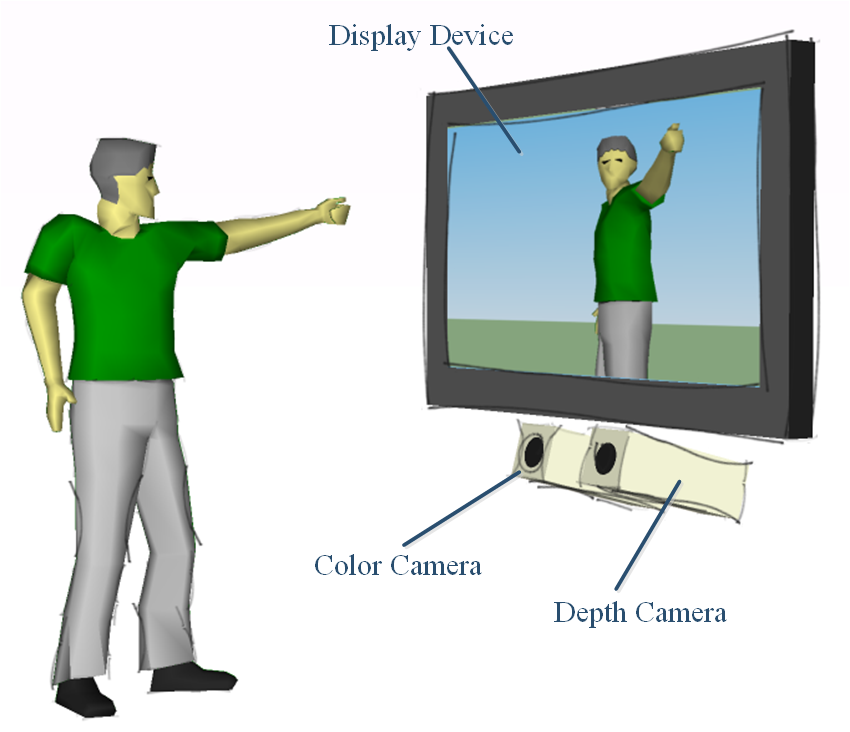
\includegraphics[width = 0.5\linewidth]{figures/3-MMC/GeneralSetup}
	}
	\subfloat[Current Implementation using Kinect]{ \label{fig:3-MMC:hardware:b}
		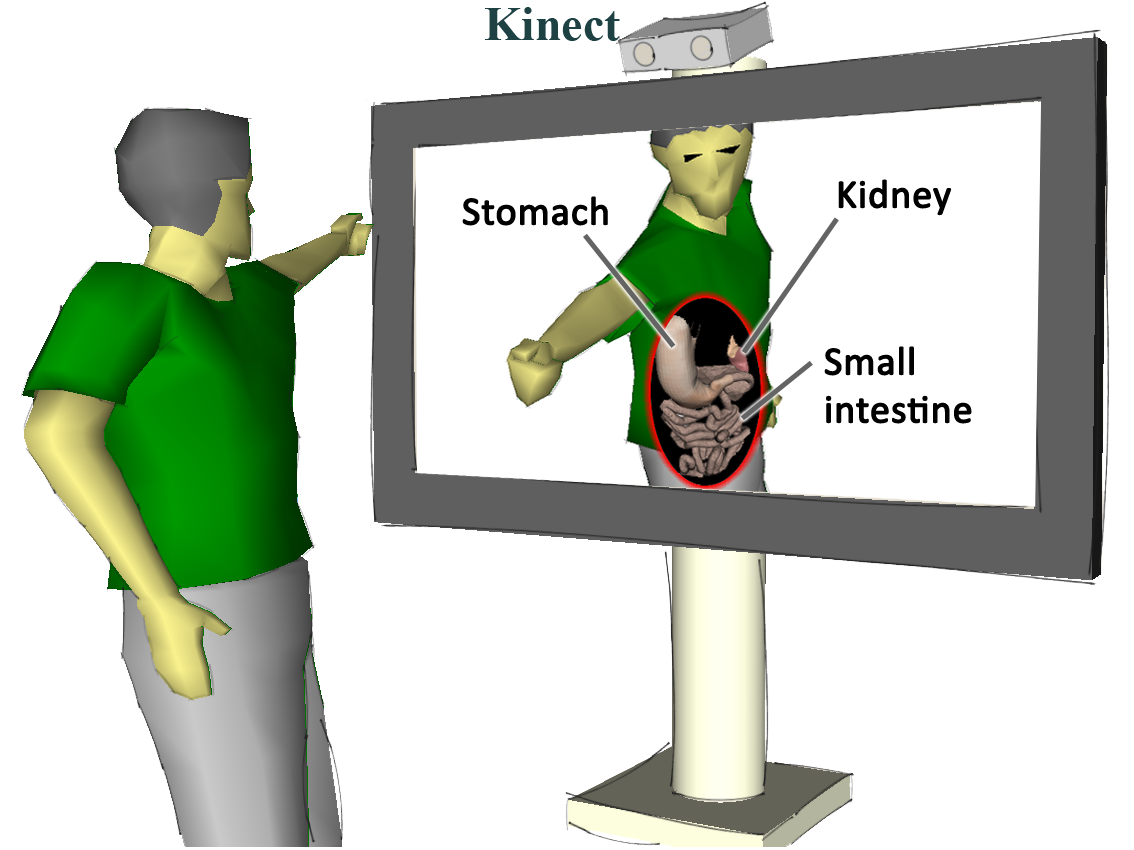
\includegraphics[width = 0.5\linewidth]{figures/3-MMC/mirracleIllustration}
	}
	\caption[Magic Mirror Hardware setup.]{Magic Mirror Hardware setup. (a) The system consists of a display, a color camera and a depth sensor. The color camera perceives the visual image, which is shown in the display to generate a mirror effect. The depth sensor observes the user and collects natural input for interaction with the system. (b) The color and depth camera are replaced by one Microsoft Kinect.}
	\label{fig:3-MMC:hardware}
\end{figure}

\subsubsection{Software framework}
The system framework of the prototype is illustrated in \figurename{\ref{fig:3-MMC:systemFramework}}.
To access the Kinect the system uses Microsoft Kinect SDK or OpenNI\footnote{\url{https://en.wikipedia.org/wiki/OpenNI}}, which is an open source software framework that allows retrieving color and depth images from the Kinect. The depth sensor is used for two purposes. First, the depth values are projected to the color image providing depth information for each pixel in the color image. Second, a skeleton tracking algorithm uses the depth image to track the pose of multiple joints of a user who is standing in front of the camera. For skeleton tracking the Magic Mirror uses NITE a software by PrimeSense that performs gesture recognition and skeleton tracking based on depth images. NITE can be used with the Kinect through the OpenNI framework.
\begin{figure}
	\centering
	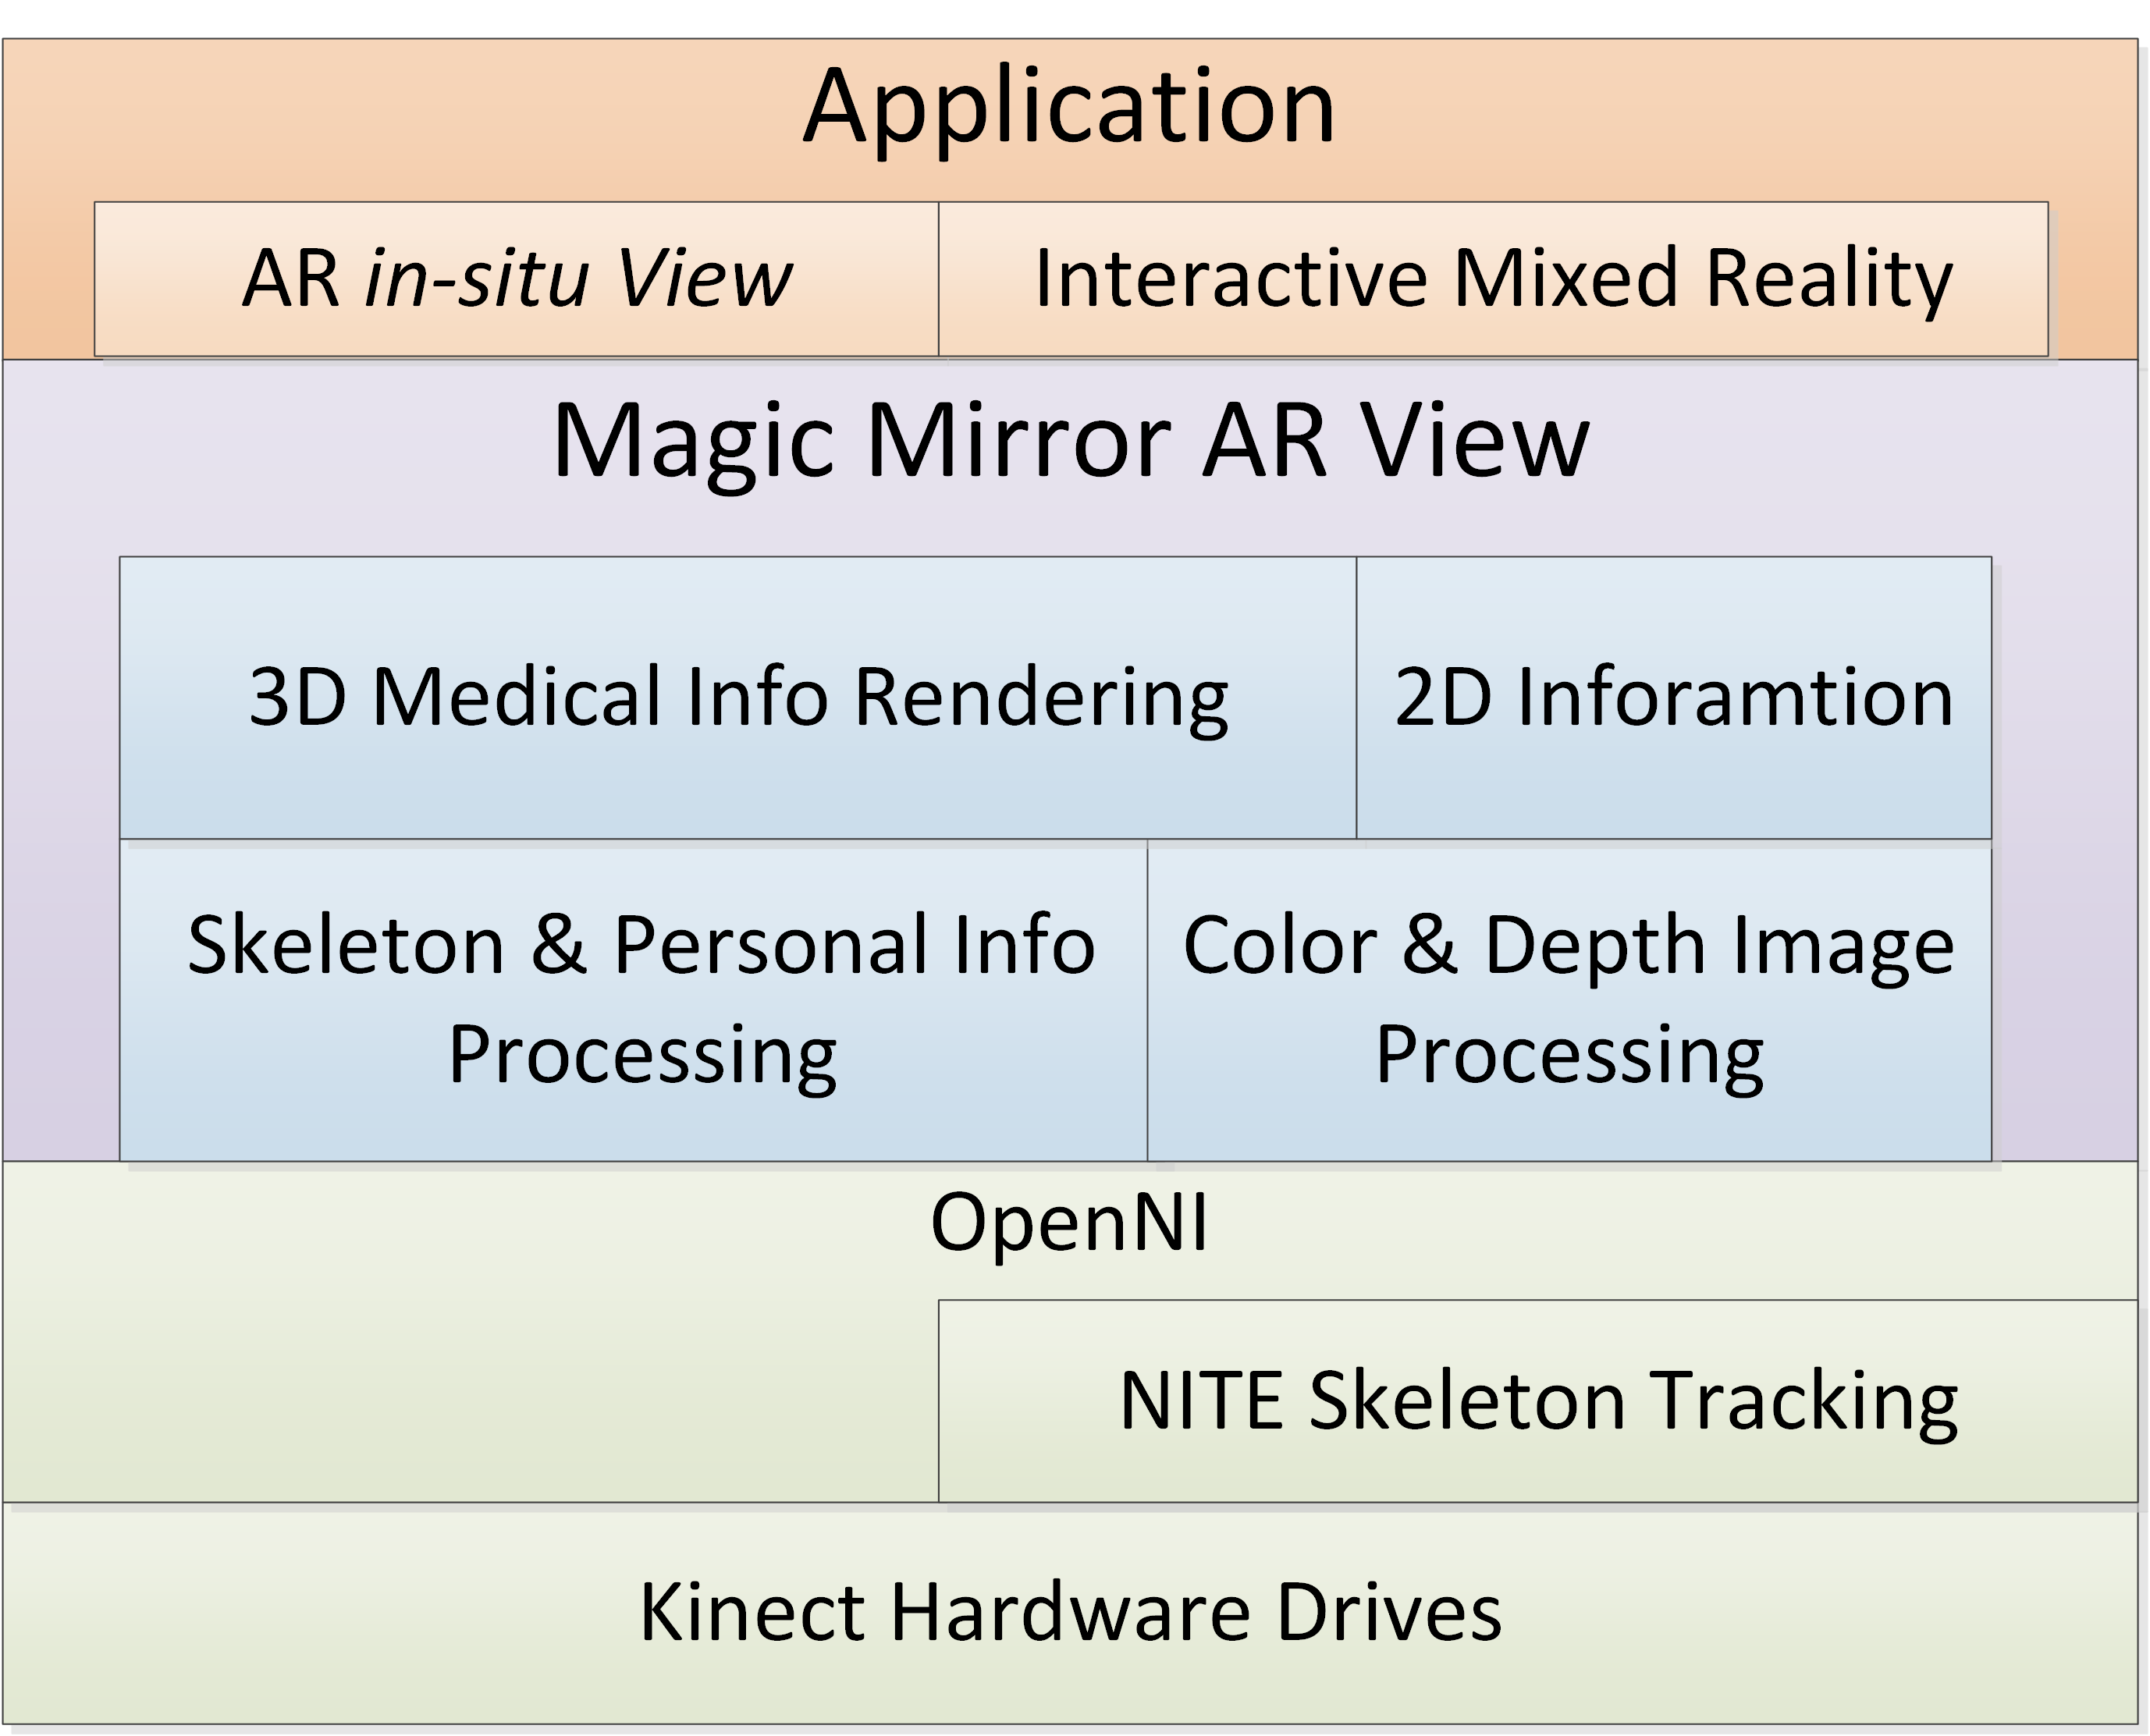
\includegraphics[width = 0.7\linewidth]{figures/3-MMC/SystemFramework}
	\caption[Magic Mirror system framework]{Magic Mirror system framework. The lowest two layers represent the open source library to access the Kinect raw image data and skeleton information. The middle layer is the modules used to create Magic Mirror AR view of the user. The top level is the application with basic system features.}
	\label{fig:3-MMC:systemFramework}
\end{figure}

The Magic Mirror AR view is based on the information perceived via Kinect and corresponding medical information. As shown in \figurename{\ref{fig:3-MMC:systemFramework}}, there are four modules:
%\textit{Skeleton \& Personal Information Processing}, \textit{Color \& Depth Image Processing}, \textit{3D Medical Information Rendering}, and \textit{2D Information} to generate the mirror-like effect and non-physical visual feedback.
\ul{Skeleton \& Personal Information Processing} is important to achieve personalized perception. 
\ul{Color \& Depth Image Processing} is the basic module to generate the mirror-like effect and merge the non-physical visual outcome. \ul{3D Medical Information Rendering} processes the corresponding 3D medical images or models and generates virtual elements for the Magic Mirror AR view and it can employ OpenGL and OpenGl Shading Language, and any other 3D rendering libraries, e.g. Coin3D. \ul{2D Information} includes window management and basic user interface elements, such as 2D text and image information, and it can be implemented using Qt.

The applications based on the \textit{Magic Mirror AR View} has two important features, \textbf{AR \textit{in-situ} view} and \textbf{Interactive Mixed Reality}. The blue rectangles represent the basic visualization functions of the system, which would be discussed in details later. The prototype system discussed in this section is a personalized Magic Mirror system for anatomy learning (see \figurename{\ref{fig:3-MMC:Prototype}). 
%It focuses on important organs of the thorax and abdomen and the bones. The system can currently provide MR \textit{in-situ} visualization, render skeleton from an original CT-volume, and showcase 3D models of organs. The sensor tracks the user positions in real-time, and contextual \textit{in-situ} visualization algorithms enable the augmentation of organs and bones directly onto the user body.

\subsubsection{Medical Information}
Aside from text and 2D atlas, 3D volumes and models are also important methodologies to represent medical information. The common way in medicine is to use 3D volumes, where we have one pixel or voxel for every point in 3D. This is the kind of data we get from CT or MRI. The other ones are polygonal or surface models, where only the surface (e.g. skin or the surface of the organ) is stored. For models that have been created for education often surface models are used because they look better.
While the system can use a CT or MRI scan, it doesn't make sense to acquire a CT or MRI scan of the user if it is not required for medical reasons. Therefore, we augment the medical volume from the Visible Korean Human dataset (VKH) \cite{Park2006} onto the user. This dataset consists of a CT scan, a MRI volume and a photographic volume which has been acquired by stacking up cryosections. 
Most CT and MRI medical images are saved in the DICOM standard, which is the format that is used in all hospitals. Unfortunately, most software for research does not support DICOM. The Magic Mirror system takes a ``\textit{$\ast$.MHD}'' file as the medical data. One drawback of the volume data is that the 3D dataset cannot be deformed in real-time. So if the user bends, this is not reflected in the visualization of the medical data and also movements of the limbs are not visualized correctly. While later, possible solutions to address this issue are discussed, for the current system, which focuses on the abdominal area, this is a minor problem.

Visualizing structures other than bones from the CT is more challenging. In a first attempt, the segmentation that is available for the CT volume was used to visualize different organs in the abdominal area. The quality of the visualization was low, as the segmentation does not have sub-pixel accuracy and transfer-functions on CT intensities cannot provide a visualization with realistic colors and textures of organs. Therefore instead of using the volumetric data, additional polygonal models were integrated. The Anatomium\footnote{\url{www.anatomium.com}} dataset provides polygonal models of many organs of the human body. A scene graph including multiple organs was extracted from the dataset. Using Coin3D this scene graph is augmented onto the user. The simultaneous visualization of bones from CT and a polygonal model of the small intestine is shown in \figurename{\ref{fig:3-MMC:Mirracle}}.
	
\subsection{Personalized perception and interaction} \label{sec:3:MMCInteraction}
To create a Magic Mirror AR view for anatomy leaning, special medical data should be selected from the database and transformed based on current user's personal information and interaction (see \figurename{\ref{fig:3-MMC:MedicalInfoFlow}}). Then the data is processed to generate the non-physical visual effect, merging with the mirror-like color image based on the depth information. The user learns anatomy knowledge via perception of the AR view of their own body. Interaction can also be performed by the user intentionally or unintentionally to control the  selection and transformation of the medical information, enabling an interactive AR view.
\begin{figure}
	\centering
	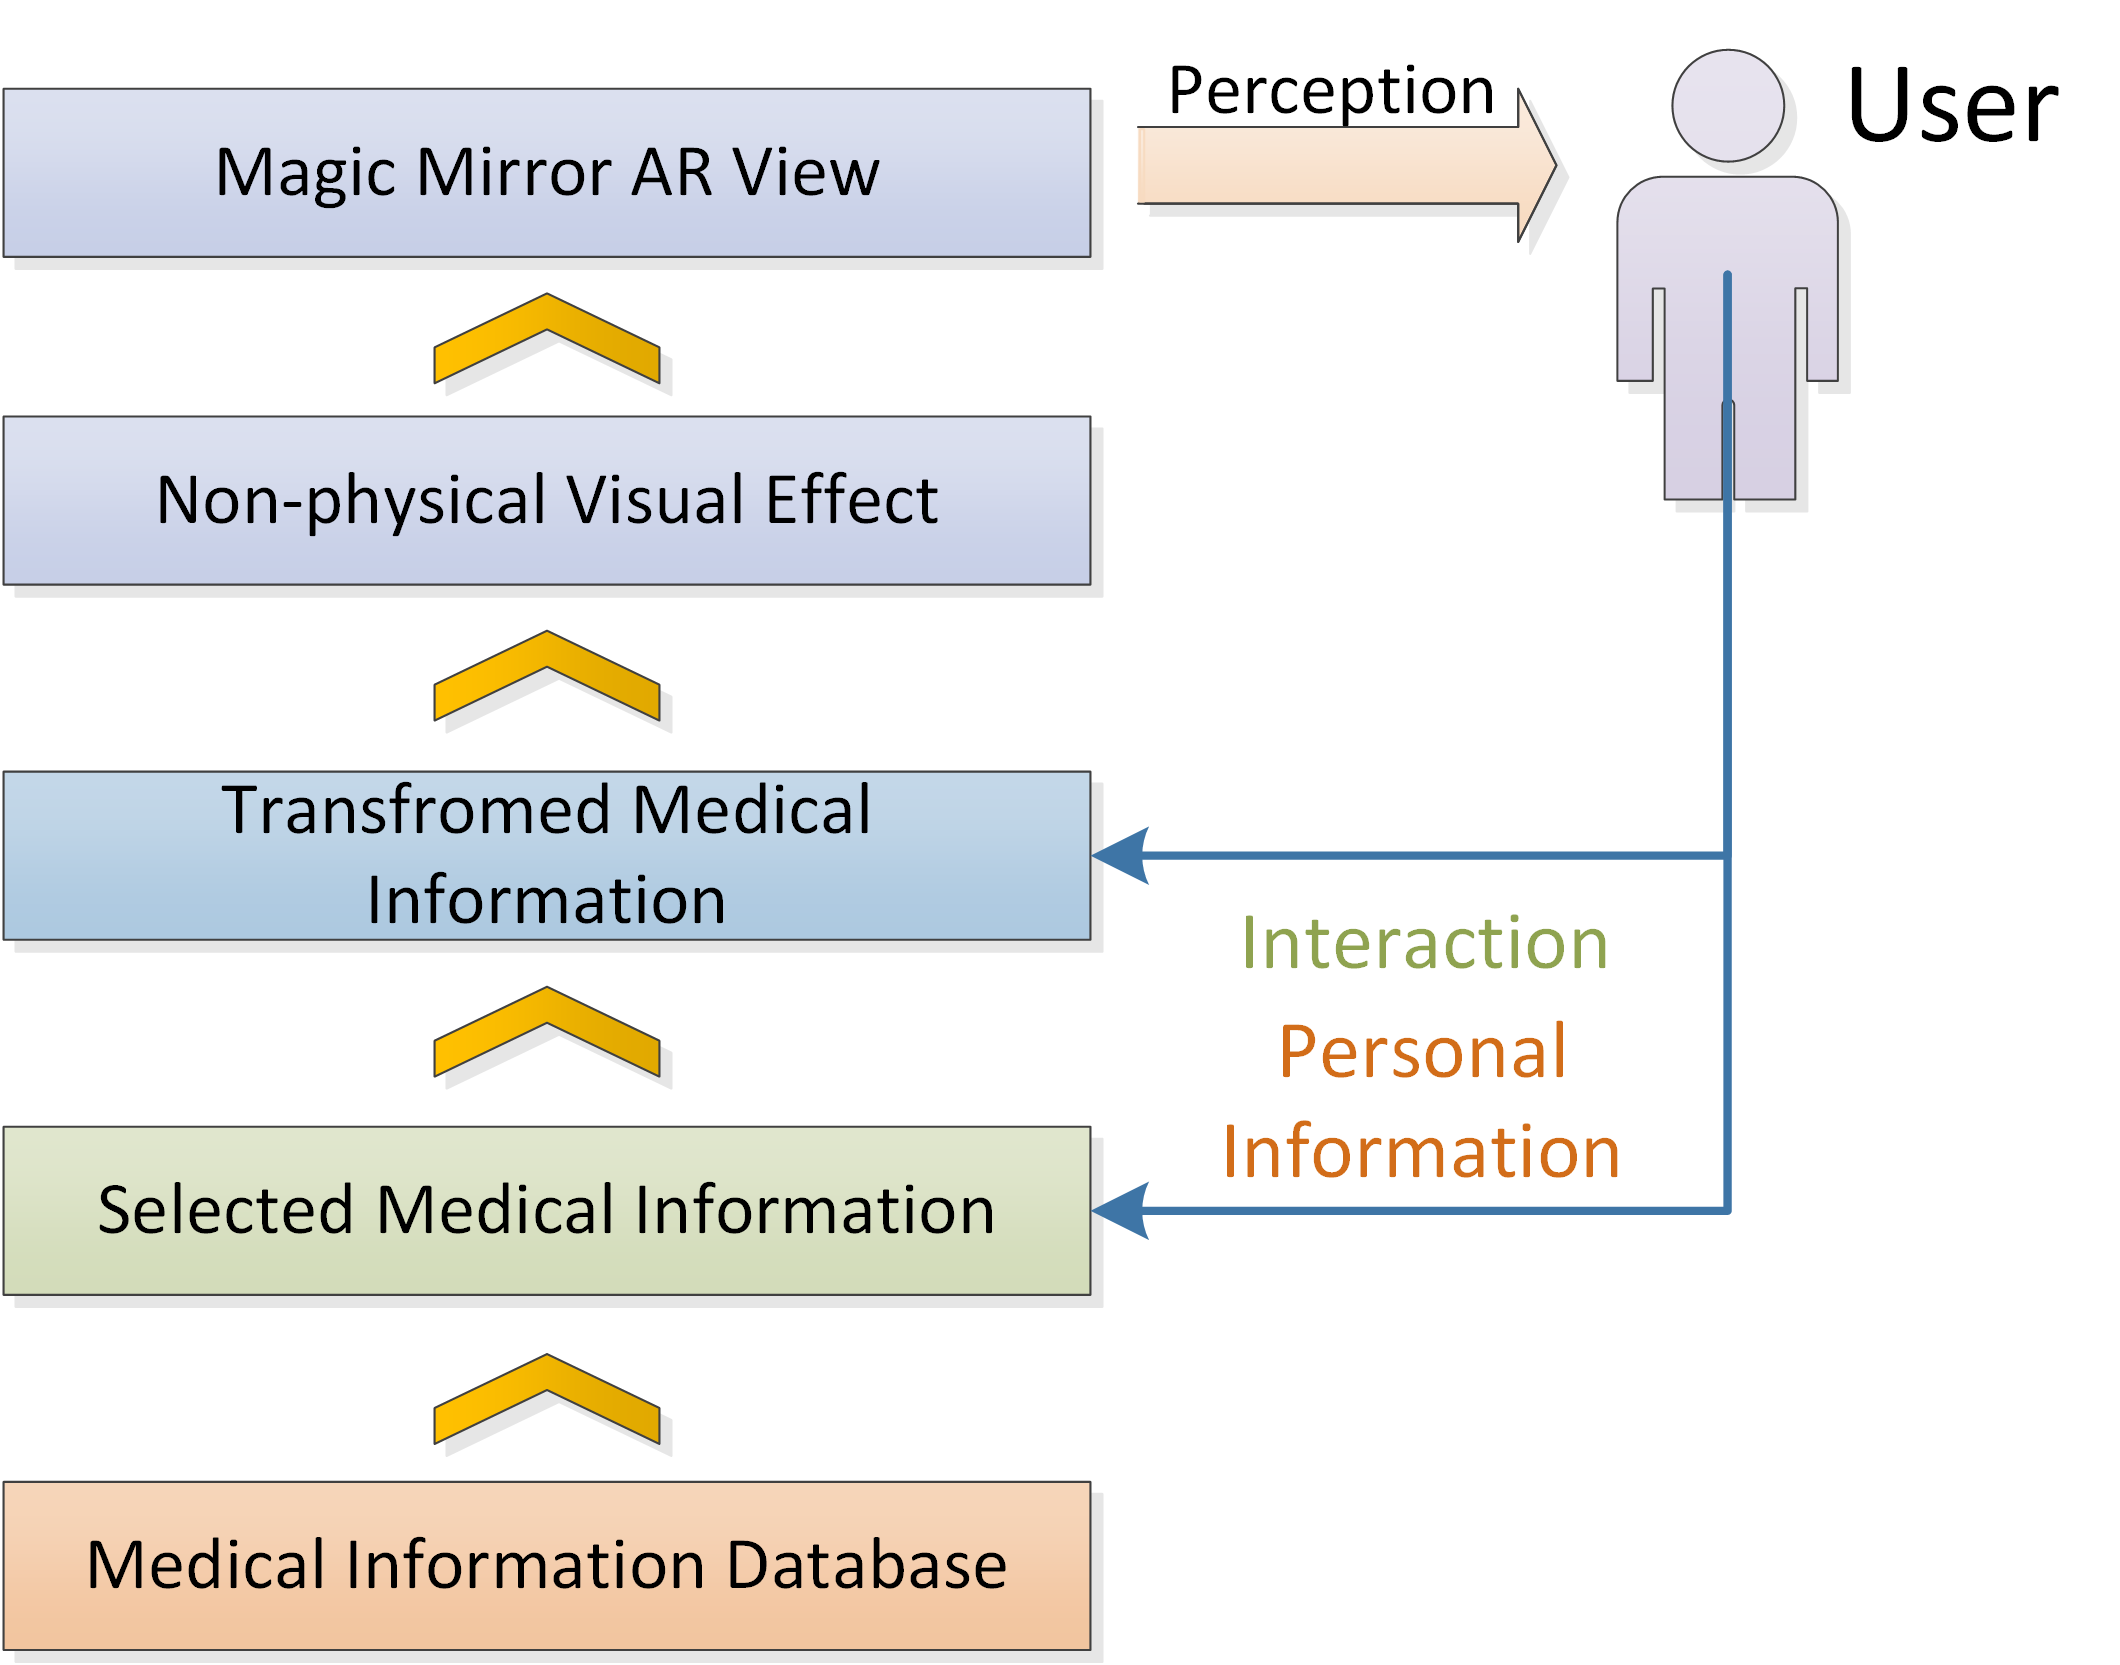
\includegraphics[width=0.7\linewidth]{figures/3-MMC/MedicalInfoFlow}
	\caption[Medical Information Flow]{For each non-physical visual effect, corresponding medical information is selected from the medical information database, transformed, and rendered according to the function setting and the user's interaction and personal information. Finally, the Magic Mirror AR view is generated.}
	\label{fig:3-MMC:MedicalInfoFlow}
\end{figure}

\subsubsection{Calibration of the user}
The skeleton tracking algorithm has to calibrate the user. For this, the user has to take a certain pose and hold it for several seconds. This calibration estimates the individual distances between joints for each user. This allows estimating the size of the user. The 3D volume and models are scaled to the size of the user and augmented onto the user.  
The NITE skeleton tracking algorithm, which is used in the Magic Mirror system, also requires the user to calibrate before the tracking works. In order to build a system that people can use without further instruction, we need to attract their attention and develop a self-explaining system. The NITE skeleton tracking provides a pixel map, where all pixels that belong to a person are labeled, before the user is calibrated. We use this to attract the attention of people passing by. As soon as someone walks into the field of view of the camera, that person is augmented with green color. The user has to take a calibration pose to become tracked. The system augments a silhouette of a person taking the calibration pose onto the display and asks the user to take the same pose. After calibration ends the system prints a message telling that a user has been recognized and the AR view can then be generated.

\subsubsection{AR in-situ visualization of human anatomy}
For a personalized visualization of organs the concept of a Magic Mirror is employed. The camera image is flipped horizontally and shown on the screen such that the user has the impression of standing in front of a real mirror. The system tracks all user movements using a depth camera and detects the pose of the user. Then, virtual elements are added to the image of the real scene. The augmentation context visualization \cite{Bichlmeier2007} is used, such that the virtual objects are only seen through a circular focus window (see \figurename{\ref{fig:3-MMC:Mirracle}). This leads to a better perception of depth, compared to a simple augmentation of the whole CT. 
By using the Magic Mirror metaphor, the user is led to believe that he or she is able to look inside their own body. At the same time, different medical information (CT data and a fully segmented dataset of cross-sectional photographs of the human body) can be displayed \cite{Blum2012}. For visualization of the bones a transfer function is used as bone can be distinguished easily in the CT volume based on the voxel intensities. For some applications where CT dataset of the user is available, it can directly augment the CT dataset onto their own body to improve the perception.
\begin{figure}
	\centering
	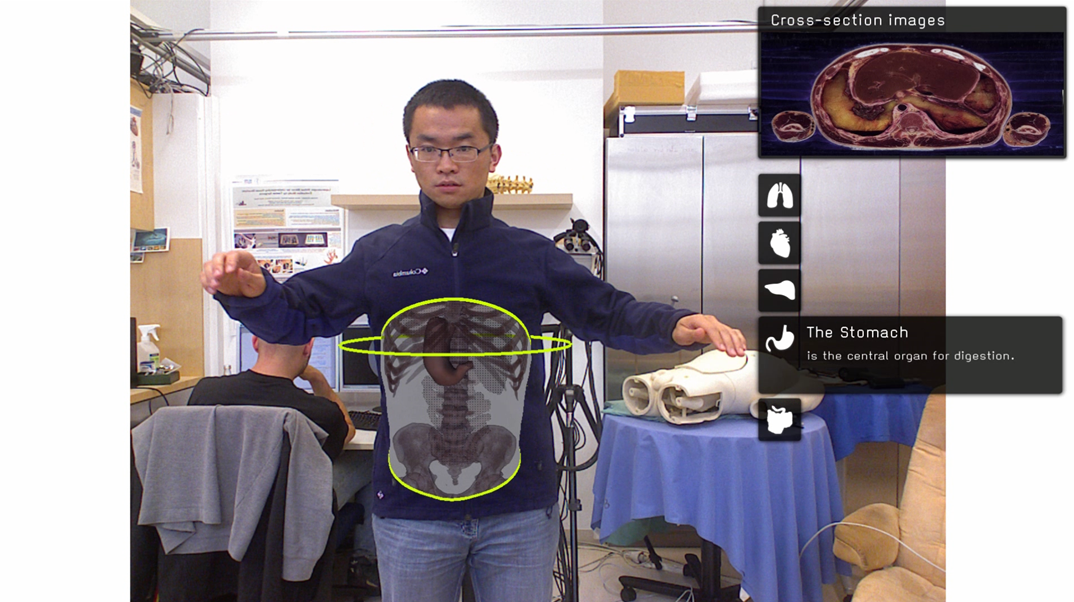
\includegraphics[width=0.9\linewidth]{figures/3-MMC/Mirracle}
	\caption{Magic Mirror Demo. The AR \textit{in-situ} visualization of human anatomy in the prototype Magic Mirror demo.}
	\label{fig:3-MMC:Mirracle}
\end{figure}

\paragraph{Presentation of additional medical information}
In addition to the AR \textit{in-situ} visualization of anatomy, the system still has to show more detailed information via text, images and 3D models. To achieve this, the system switches to a mode, where the whole screen is used to display additional information about anatomical structures, such as the 2D slices from the CT or photographic volume.
Therefore, the system can switch to the 2D or the 3D models mode as needed, and both 3D view or 2D information can be displayed to improve the perception of the medical information.

\subsubsection{Natural user interaction}
All the body movements are tracked and can be directly employed for the interaction. Arm and hand gestures are used to perform interaction in the Magic Mirror MR environment.

\paragraph{Relocating the see-through window}
The \textit{see-through} window plays an important role in creating the personalized \textit{in-situ} visualization of the anatomy.
As shown in \figurename{\ref{fig:3-MMC:NUI:a}}, the window position is controlled by the hand position. A user specific offset vector is added to the left hand joint to calculate the window position. This interactive function motivates the user to learn where the interesting organ is. For public demos for children, we limited the window position in one dimension (see \figurename{\ref{fig:3-MMC:Mirracle}) and the user moves up or down to change the window position to show different organs in the corresponding planes.
	
\begin{figure}
	\centering
	\subfloat[Relocating \textit{see-through} window]{ \label{fig:3-MMC:NUI:a}
		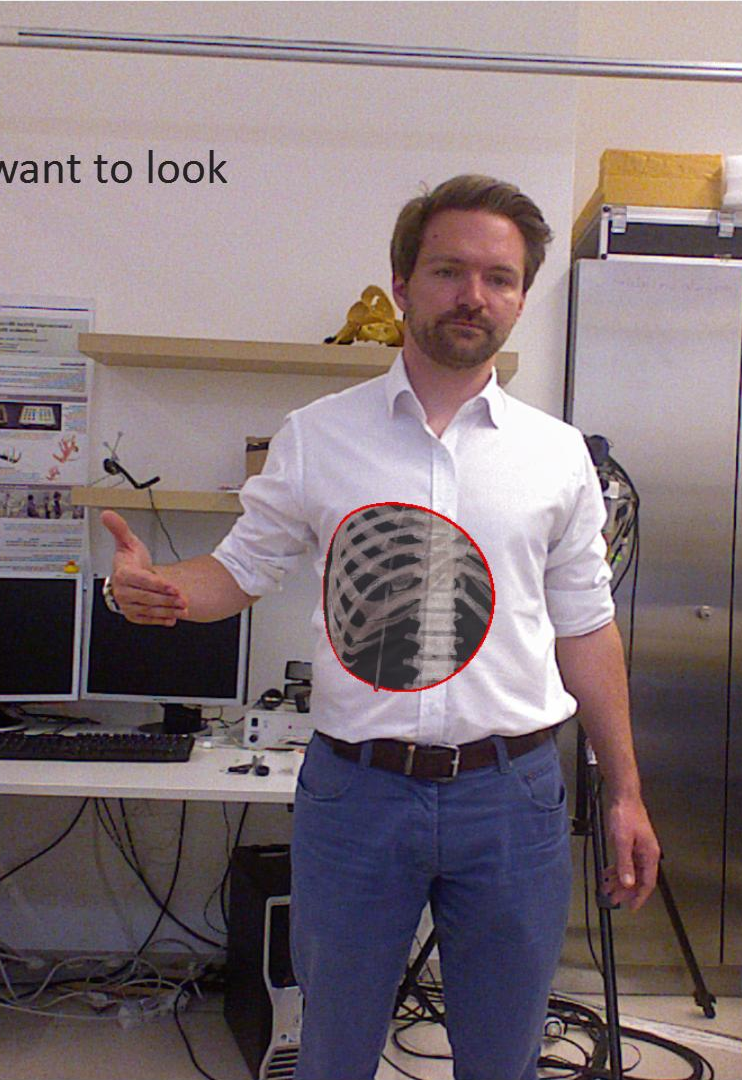
\includegraphics[height = 7cm]{figures/3-MMC/ChooseWindow}
	}
	\subfloat[Gesture-based interaction for slices]{\label{fig:3-MMC:NUI:b}
		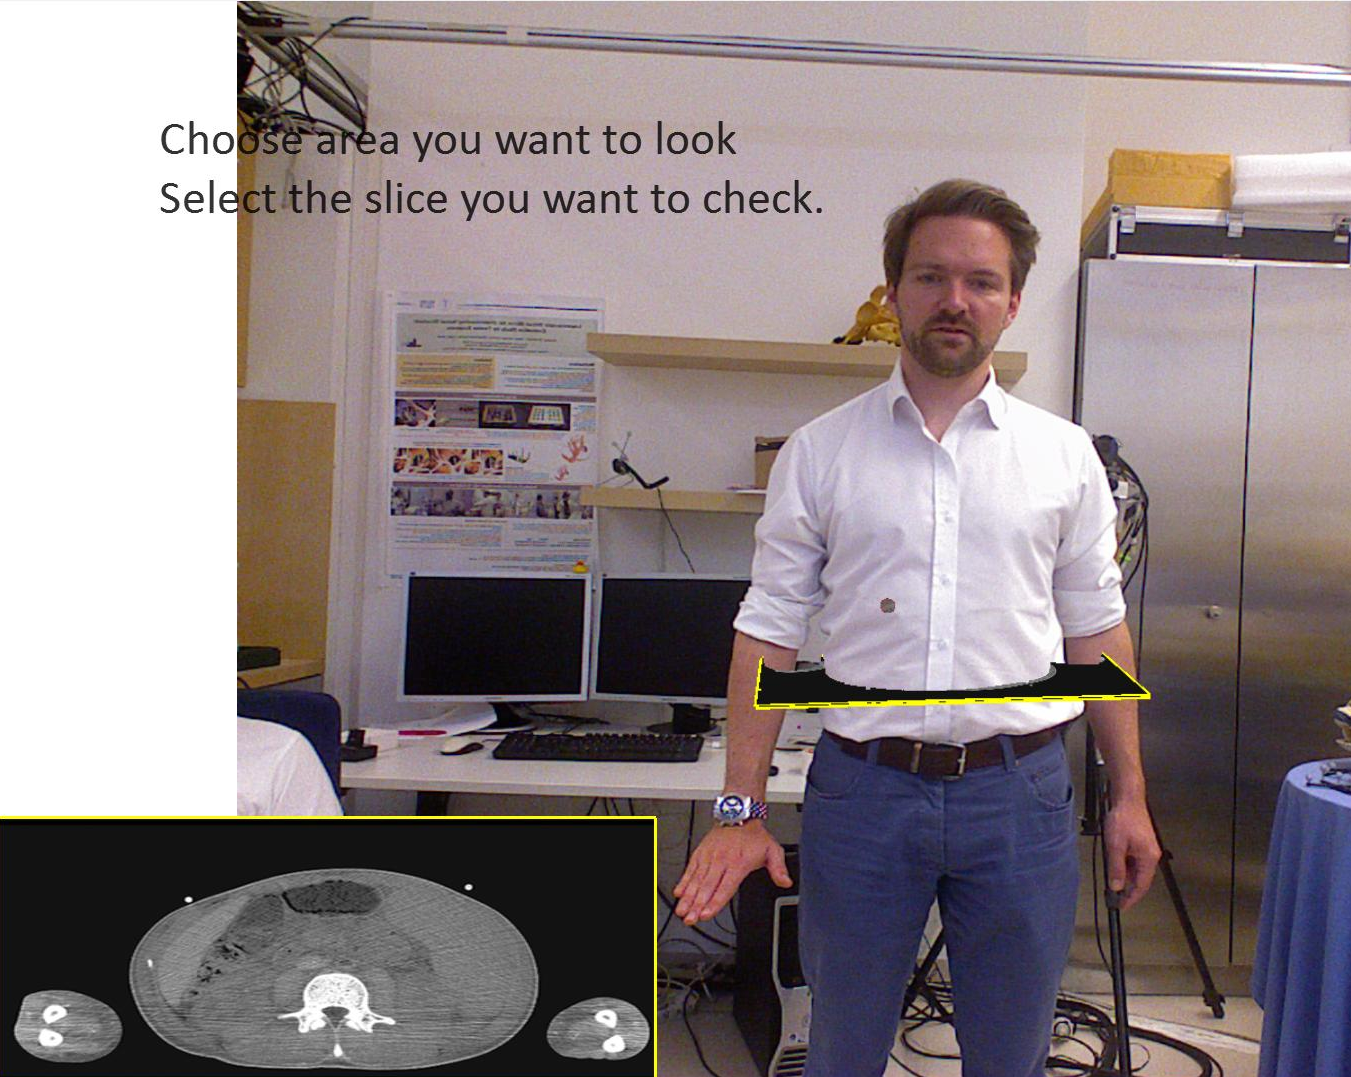
\includegraphics[height = 7cm]{figures/3-MMC/slicing}
	}
	\caption[Natural User interaction]{Arm and hand gestures can also be used to perform interaction with the Magic Mirror AR view. (a) The user can move the hand to relocate the \textit{see-through} window. (b) When the system is in the transverse slice mode, the user could move their hand up or down to choose the interesting slice image. }
	\label{fig:3-MMC:NUI}
\end{figure}
\paragraph{Gesture-based interaction for slices} A volume can be seen as a stack of transverse slices starting from the top and going to the bottom. Usually medical volumes are checked slice by slice to get the desired information. The current slice is depicted on one corner of the monitor while a yellow circle or rectangle is augmented onto the user depicting the slice plane.
The user can move their hand up or down to choose the interesting slice image (see \figurename{\ref{fig:3-MMC:Mirracle} and \figurename{\ref{fig:3-MMC:NUI:b}) when the system is in the transverse slice mode. It is similar for the sagittal slice mode. The system can easily switch slices between the CT and the photographic volume.
		
There is a trend toward competency-based education in medicine. Instead of defining a curriculum, learning outcomes are defined. Students have to fulfill these learning outcomes. The advantage of competency-based education is that all students will have the same competency in the end. A student who is less skilled has to take more time to learn than a student who already has good skills. One requirement for this is that the students have to be able to educate themselves until they reach the required competency. 
%We plan to use the AR Magic Mirror system both to allow them to do training and to test whether a learning outcome has been met. 
This framework can be made easily available to them so that they can use it for training and testing at any time.
	
\subsection{Evaluation of the framework}
The current system allows visualization of static anatomy on the user and offers a simple user interface to select CT or photographic slices. Demos of the prototype have been given on various public occasions. Medical doctors (MD) from physiotherapy, anatomy, radiology, sports medicine, children's medicine, and medical teacher and science centers are interested in using such a system in education of medical students and pupils. 
As an augmented reality anatomy learning application, system usability are very important prior to its translation in classroom. We undertook one user study involving first year medical students to verify the learning potential and acceptability of our technology as a compliment to atlas textbooks in classroom.

\paragraph{Learning Scenario} A list of questions are developed by the medical partners. Each question asks for the location of an anatomical structure. 
In the first step the student has to position the focus window at the correct location via the function ``Relocating the see-through window''. After positioning the window, the distance to the actual position of the structure is computed. If the distance exceeds a threshold it is considered as wrong. In this case the student has to reposition the focus window. When the correct position has been selected, the focus window is fixed and another mode is activated where a more fine grained selection is possible using ``Gesture-based interaction for slices''. 
In each question either one or more of the correct slices along the three directions have to be found. 
%After a set of questions are answered, a score is presented, which is based on the number of tries and the time a student required to find the correct slices.

\paragraph{Participants:} 72 medical students from the Anatomische Anstalt der Ludwig-Maximilians-Universit\"at M\"unchen, having an age range between 21yrs and 28yrs, were enrolled in this study. The distribution of gender was 38 male and 34 female. Their medical experience was: 50 participants did not have any expertise, 8 had paramedic training, 5 with healthcare training, and 9 with some other degree (e.g. biology, chemistry, and therapy). 

\paragraph{Analysis:} Responses to questions were based on a four point Likert Scale: (1) \textit{strongly disagree}, (2) \textit{disagree}, (3) \textit{agree}, and (4) \textit{strongly agree}. For statistical analysis, the response categories were reduced to Yes/No: Yes (\textit{agree} + \textit{strongly agree}); No (\textit{strongly disagree} + \textit{disagree}).

The study procedure involved every participant to use the personalized Magic Mirror system for 15 minutes and try all available system functions. Participants were then asked to assess the learning potential of the technology by responding to the following questions:
\begin{itemize}
	\item[Q1-] is the system helpful for anatomy learning?  
	\item[Q2-] do you like to use the Magic Mirror? 
	\item[Q3-] is the presentation and visualization of the CT volume acceptable? 
	\item[Q4-] do you like the AR view of 3D human anatomy? 
	\item[Q5-] what other information would you want to see from the 3D rendering? (Open question)
\end{itemize}
Frequencies (F) and percentages (\%) of response on the first four questions are given in \tablename{\ref{tb:3-MMC:userStudy}}. The questionnaire, focused on motivation and perception of the participants, showed statistically significant differences for all the questions. Percentages confirmed how the students accept this Magic Mirror system for anatomy learning.
\begin{table}
	\caption[User study with fresh medical students]{Frequencies and percentages of response of the medical students about the AR system.}
	\centering
	\label{tb:3-MMC:userStudy}
	\scriptsize
	\begin{center}
		\begin{tabular}{ccccccccc}
			\multicolumn{1}{c}{\space} & \multicolumn{2}{c}{\textbf{Q1}} & \multicolumn{2}{c}{\textbf{Q2}} & \multicolumn{2}{c}{\textbf{Q3}} & \multicolumn{2}{c}{\textbf{Q4}} \\
			\hline
			\space & \textit{F} &\textit{\%}& \textit{F} &\textit{\%}& \textit{F} &\textit{\%}& \textit{F} &\textit{\%} \\
			Yes & 62 & 86.1 & 60 & 83.3 & 68 & 94.4 & 66 & 91.7 \\
			No & 10 & 13.9 & 12 & 16.7 & 4 & 5.6 & 6 & 8.3 \\
			\hline
		\end{tabular}
	\end{center}
\end{table}

The results of question 5 are depicted in \tablename{\ref{tb:3-MMC:question5}. They indicate that the participants would eventually like the current Magic Mirror system to evolve to one that includes the visualization of complex anatomy models such as the vascular system, relations between different organs, extremities, etc. 
\begin{table}
	\caption[3D anatomy expected]{Frequencies and percentages of new 3D anatomy expected by the 72 medical students}
	\centering
	\label{tb:3-MMC:question5}
	\scriptsize
	\begin{center}
		\begin{tabular}{ccc}
			%\hline
			New 3D rendering functions & \textit{F} & \textit{\%} \\
			\hline
			vascular system &	19 &	26.4 \\
			relationship between different organs&	13	&18.1\\
			extremities &	10&	13.9\\
			landmarks&	6&	8.3\\
			static AR view with their body&	6	&8.3\\
			head/brain	&5	&6.9\\
			muscle&	5&	6.9\\
			others&	5&	6.9\\
			\hline
		\end{tabular}
	\end{center}
\end{table}

\subsection{Conclusion}
This section presents a personalized AR Magic Mirror framework and a prototype for anatomy education.
The prototype system creates a MR environment, which is certified useful for anatomy learning, and the majority of the medical students accepted the learning potential of the technology. 
The academic methodologies must be changed according to the advances of new technologies, but there is still a long way for this. 
Considering the benefits of the personalized and interactive AR system for motivation and perception of anatomy learning, new technologies can additionally be helpful to facilitate autonomous learning and secondarily to reduce laboratory material and instructor costs. Together with the anatomy community, we hope to initiate such discussions in integrating exciting user-specific and gaming concepts within curricula via new anatomy learning systems. 

%It was originally suggested to us that our system would have much more of an impact for medical education if it were to be translated today in medical schools and anatomy classrooms. As such, with the help of our partner and anatomy professor, we deliver the improved AR Magic Mirror to two anatomy classes within the Anatomy Department of the Ludwig Maximilian University (LMU) Medical School, Munich, Germany. 
%The anatomy professors made it clear that the proposed system is exciting, but has to go beyond state-of-the-art technology to be truly useful for education. Our participants stressed the importance of visualization of anatomy that can change dynamically resulting from the actions of the user moving the body. Furthermore, more advanced user interactions like the use of gaming elements would be required to make the use of the system for learning and rehabilitation tasks more interesting.
%todo: {Accuracy of Registration} improve the perception of the MR view via accurate registration. Anatomy learning, personal information (gender, age, body shape)
\section{Personal Registration of Magic Mirror}

\subsection{Personal Information}
We augment a personalized visualization of a CT dataset onto the user. However as full CT scans of any user are generally not available, we use the Visible Korean Human dataset (VKH), which consists of a CT scan, an MR volume and a photographic volume which has been acquired by stacking up cry sections. To allow a correct augmentation of the CT data, the gender, age, body size and pose of the user has to be detected. This is performed based on the color image using the OpenBR library \cite{Klontz2013} and the depth image using the NITE skeleton tracking software. The corresponding CT volume is chosen and scaled to the size of the user and augmented onto the user body. For visualization of the bones a transfer function is used as bones can be distinguished easily in the CT volume based on their voxel intensities. For the organs a segmentation of the VKH is used. The augmentation uses contextual in-situ visualization such that the virtual objects are only shown through a circular window. This leads to a better perception of depth, compared to a simple augmentation of the whole CT. The user could naturally turn around their body to check CT volume from different viewpoints and put their right hand at different heights to select a body plane with corresponding anatomy.

\subsection{Personal Registration}
We presents a general method to interactively improve and correct the Kinect skeleton for anatomy education purposes. We believe that our general method can be applied to projectors or other sensors as well for augmented reality. A thorough validation of our method demonstrated improved precision of anatomical landmarks and opens the avenue to future improvements in medical education. Together with the ISMAR community, we hope to initiate such discussions in integrating exciting user-interaction and gaming concepts within our system.

Our AR magic mirror relies on Kinect sensor which offers an imprecise skeleton tracking output (see \figurename{\ref{fig:3-PRMM:bonelandmarker}}). This limits the precision of our magic mirror augmentations offering users false anatomical positions overlaid onto their body, resulting in a poor medical learning environment. Alternatively, had we considered projectors to display human anatomy directly on a user’s body the same inaccuracies would exist\cite{Sun2013}. 
\begin{figure}[htb]
	\centering
	\label{fig:3-PRMM:bonelandmarker}
	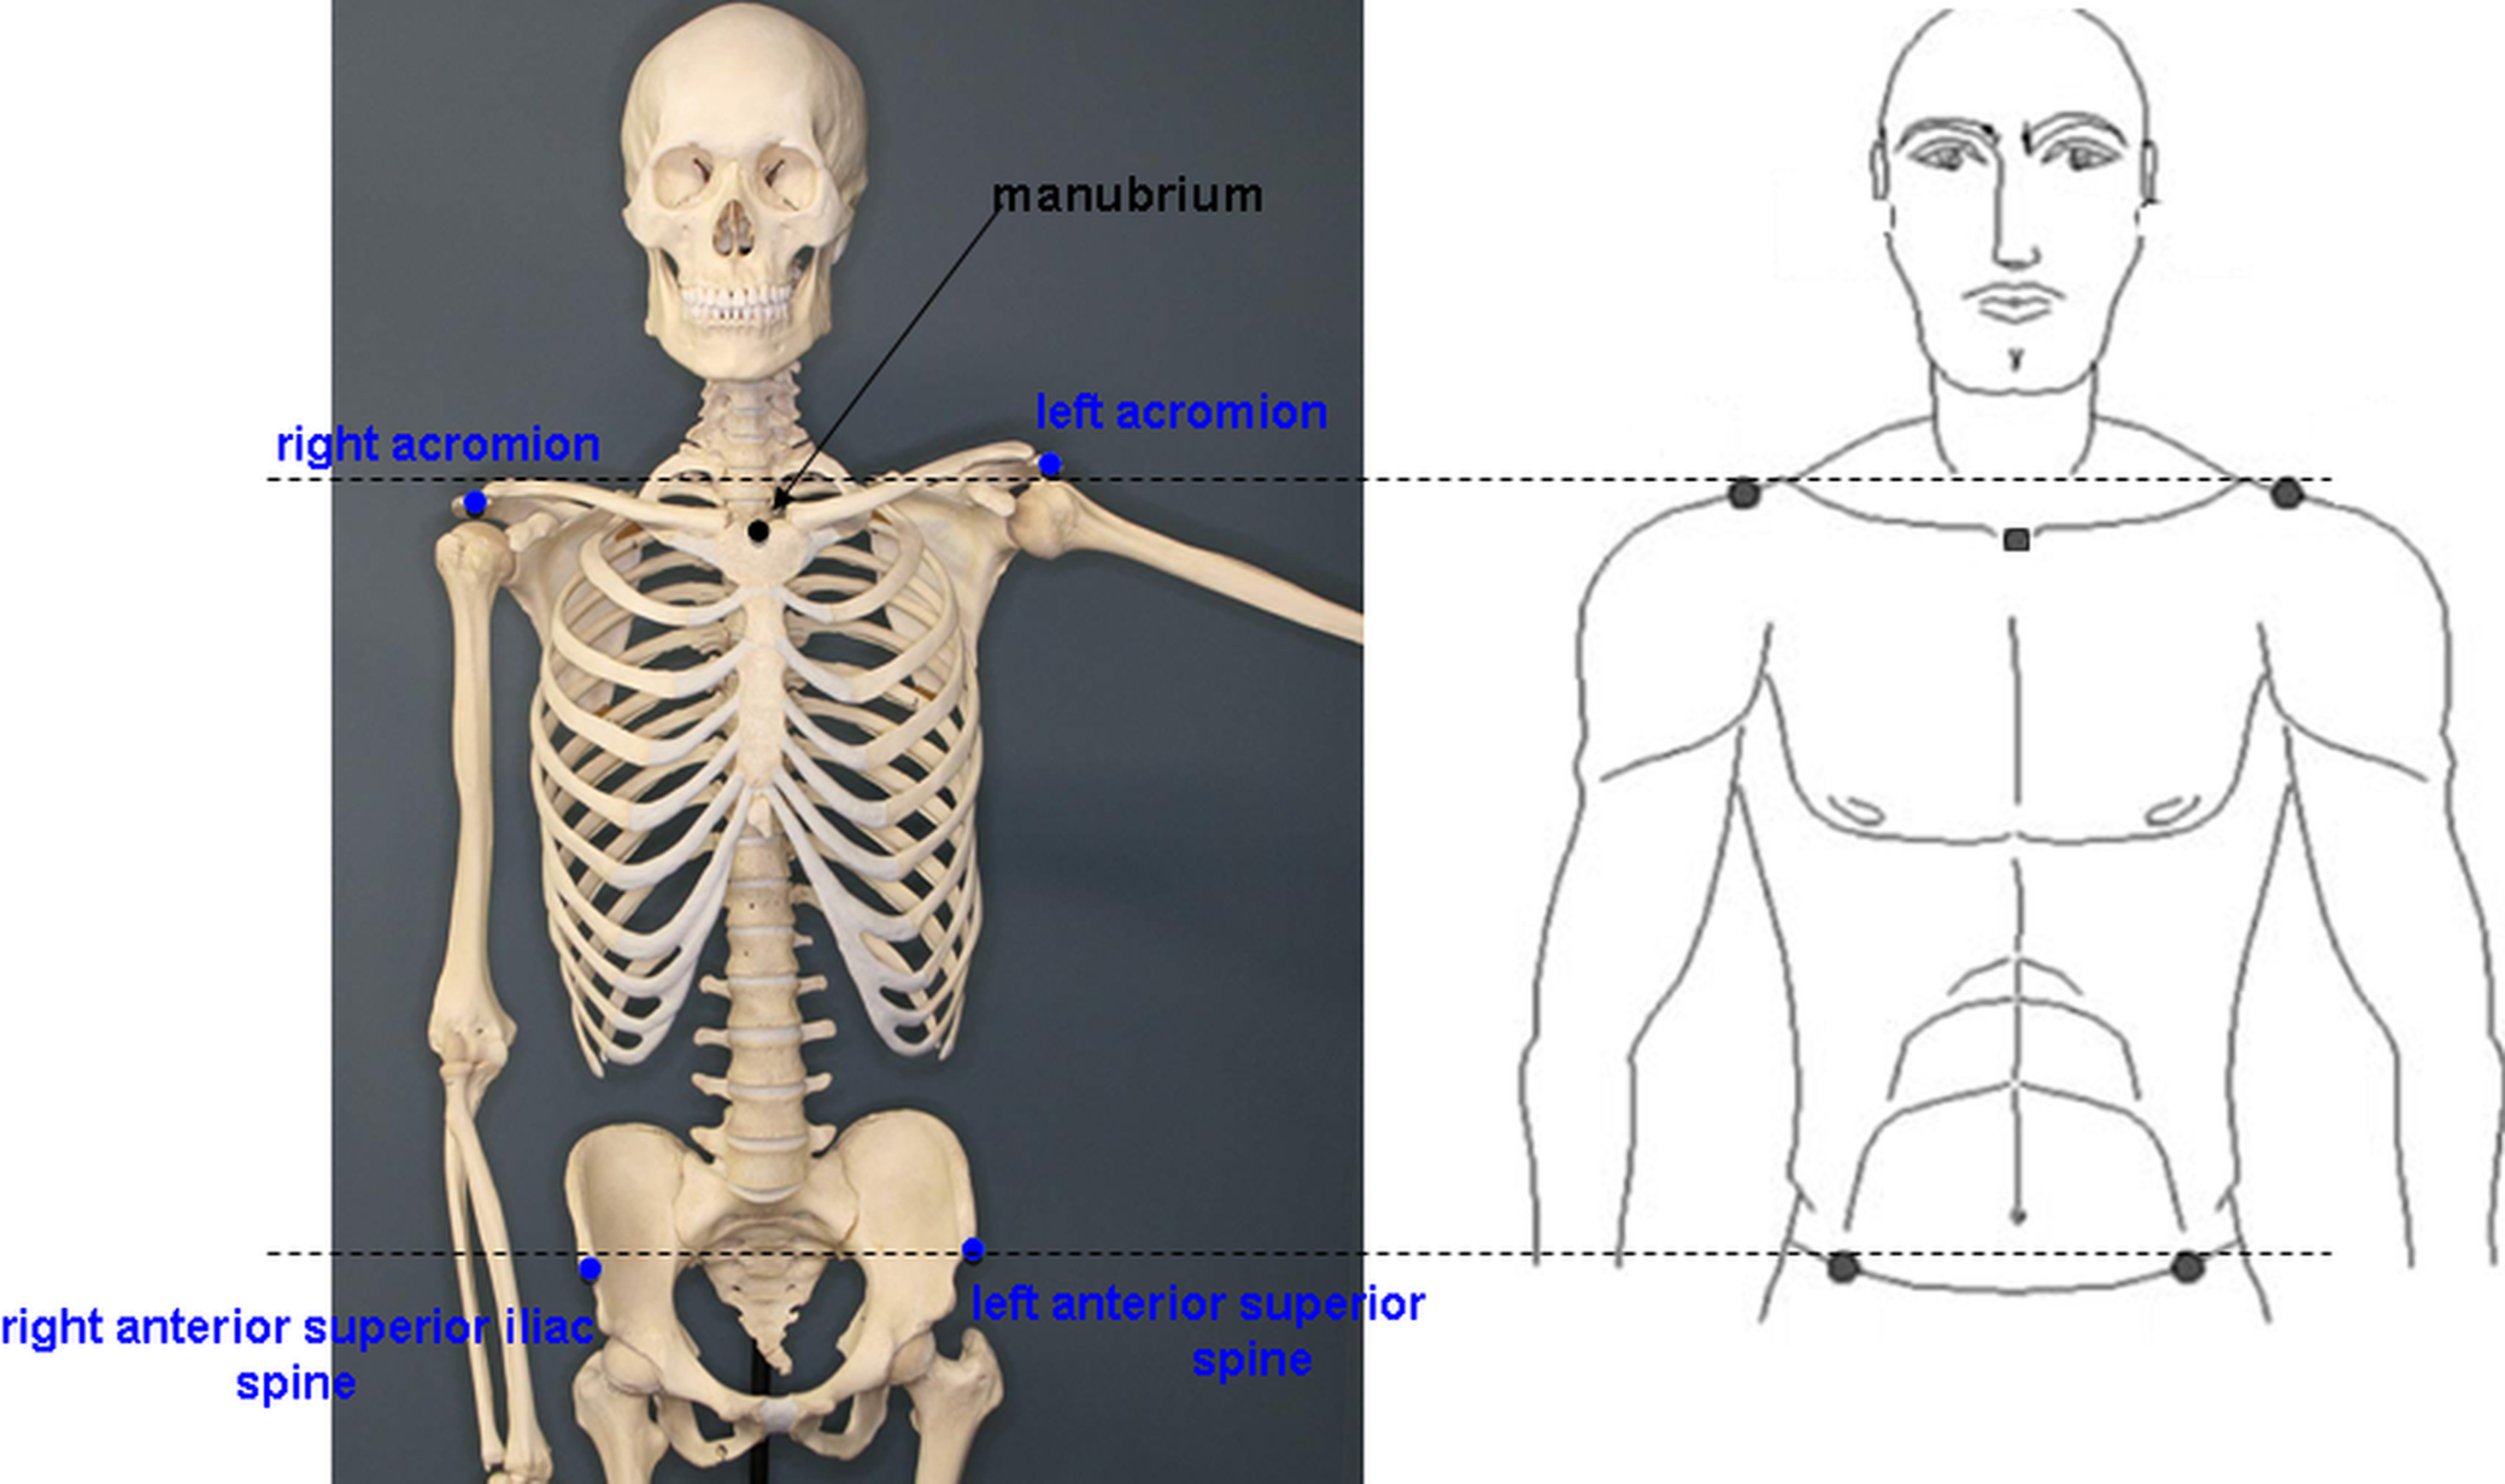
\includegraphics[width = 0.75\linewidth]{figures/3-PRMM/FiveBoneLandmarker.png}
	\caption{Selected anatomical points for Kinect skeleton improvement and subsequent CT warping and interpolation.}
\end{figure}

The goal of this method is to propose a more precise user-specific learning environment. Together with orthopedic surgeons we have defined anatomical bone landmarks: (i) which are correctly identified in medical data such as CT and (ii) which users can touch easily on their body while standing in front of any sensor. These landmark positions allow the deformation and interpolation of the medical data correctly within the magic mirror and onto the human body, resulting in a more precise Kinect skeleton and augmentation. A user study involving surgeons and anatomy experts confirm our findings. 

The skeleton output from Kinect limits the precision of the AR magic mirror applications. Thus, our magic mirror augmentations would contain errors and users would easily distinguish anatomical offsets on their body resulting in a poor anatomy learning environment. Alternatively, we had considered projectors to display human anatomy and along with their existing limitations the same inaccuracies would exist. Our aim was then to propose a method to correct for such overlay inaccuracies that could be translated to any magic mirror system worldwide. Together with orthopedic surgeons, we have defined five bone landmarks that (i) users can easily identify and touch while standing in front of the Kinect, and (ii) that are accurately and easily identified in medical data such as CT \cite{ma2013ismar}. These are: left and right acromion, left and right anterior superior iliac spine, and the manubrium (see \figurename{\ref{fig:3-PRMM:5points}}).


\begin{figure}
	\centering
	\subfloat[~Improvement of Kinect skeleton]{
		\includegraphics[height = 7cm]{figures/3-PRMM/ModifiedSkeleton.png}
		}
	\quad
	\subfloat[~Bone landmarker in CT volume]{
		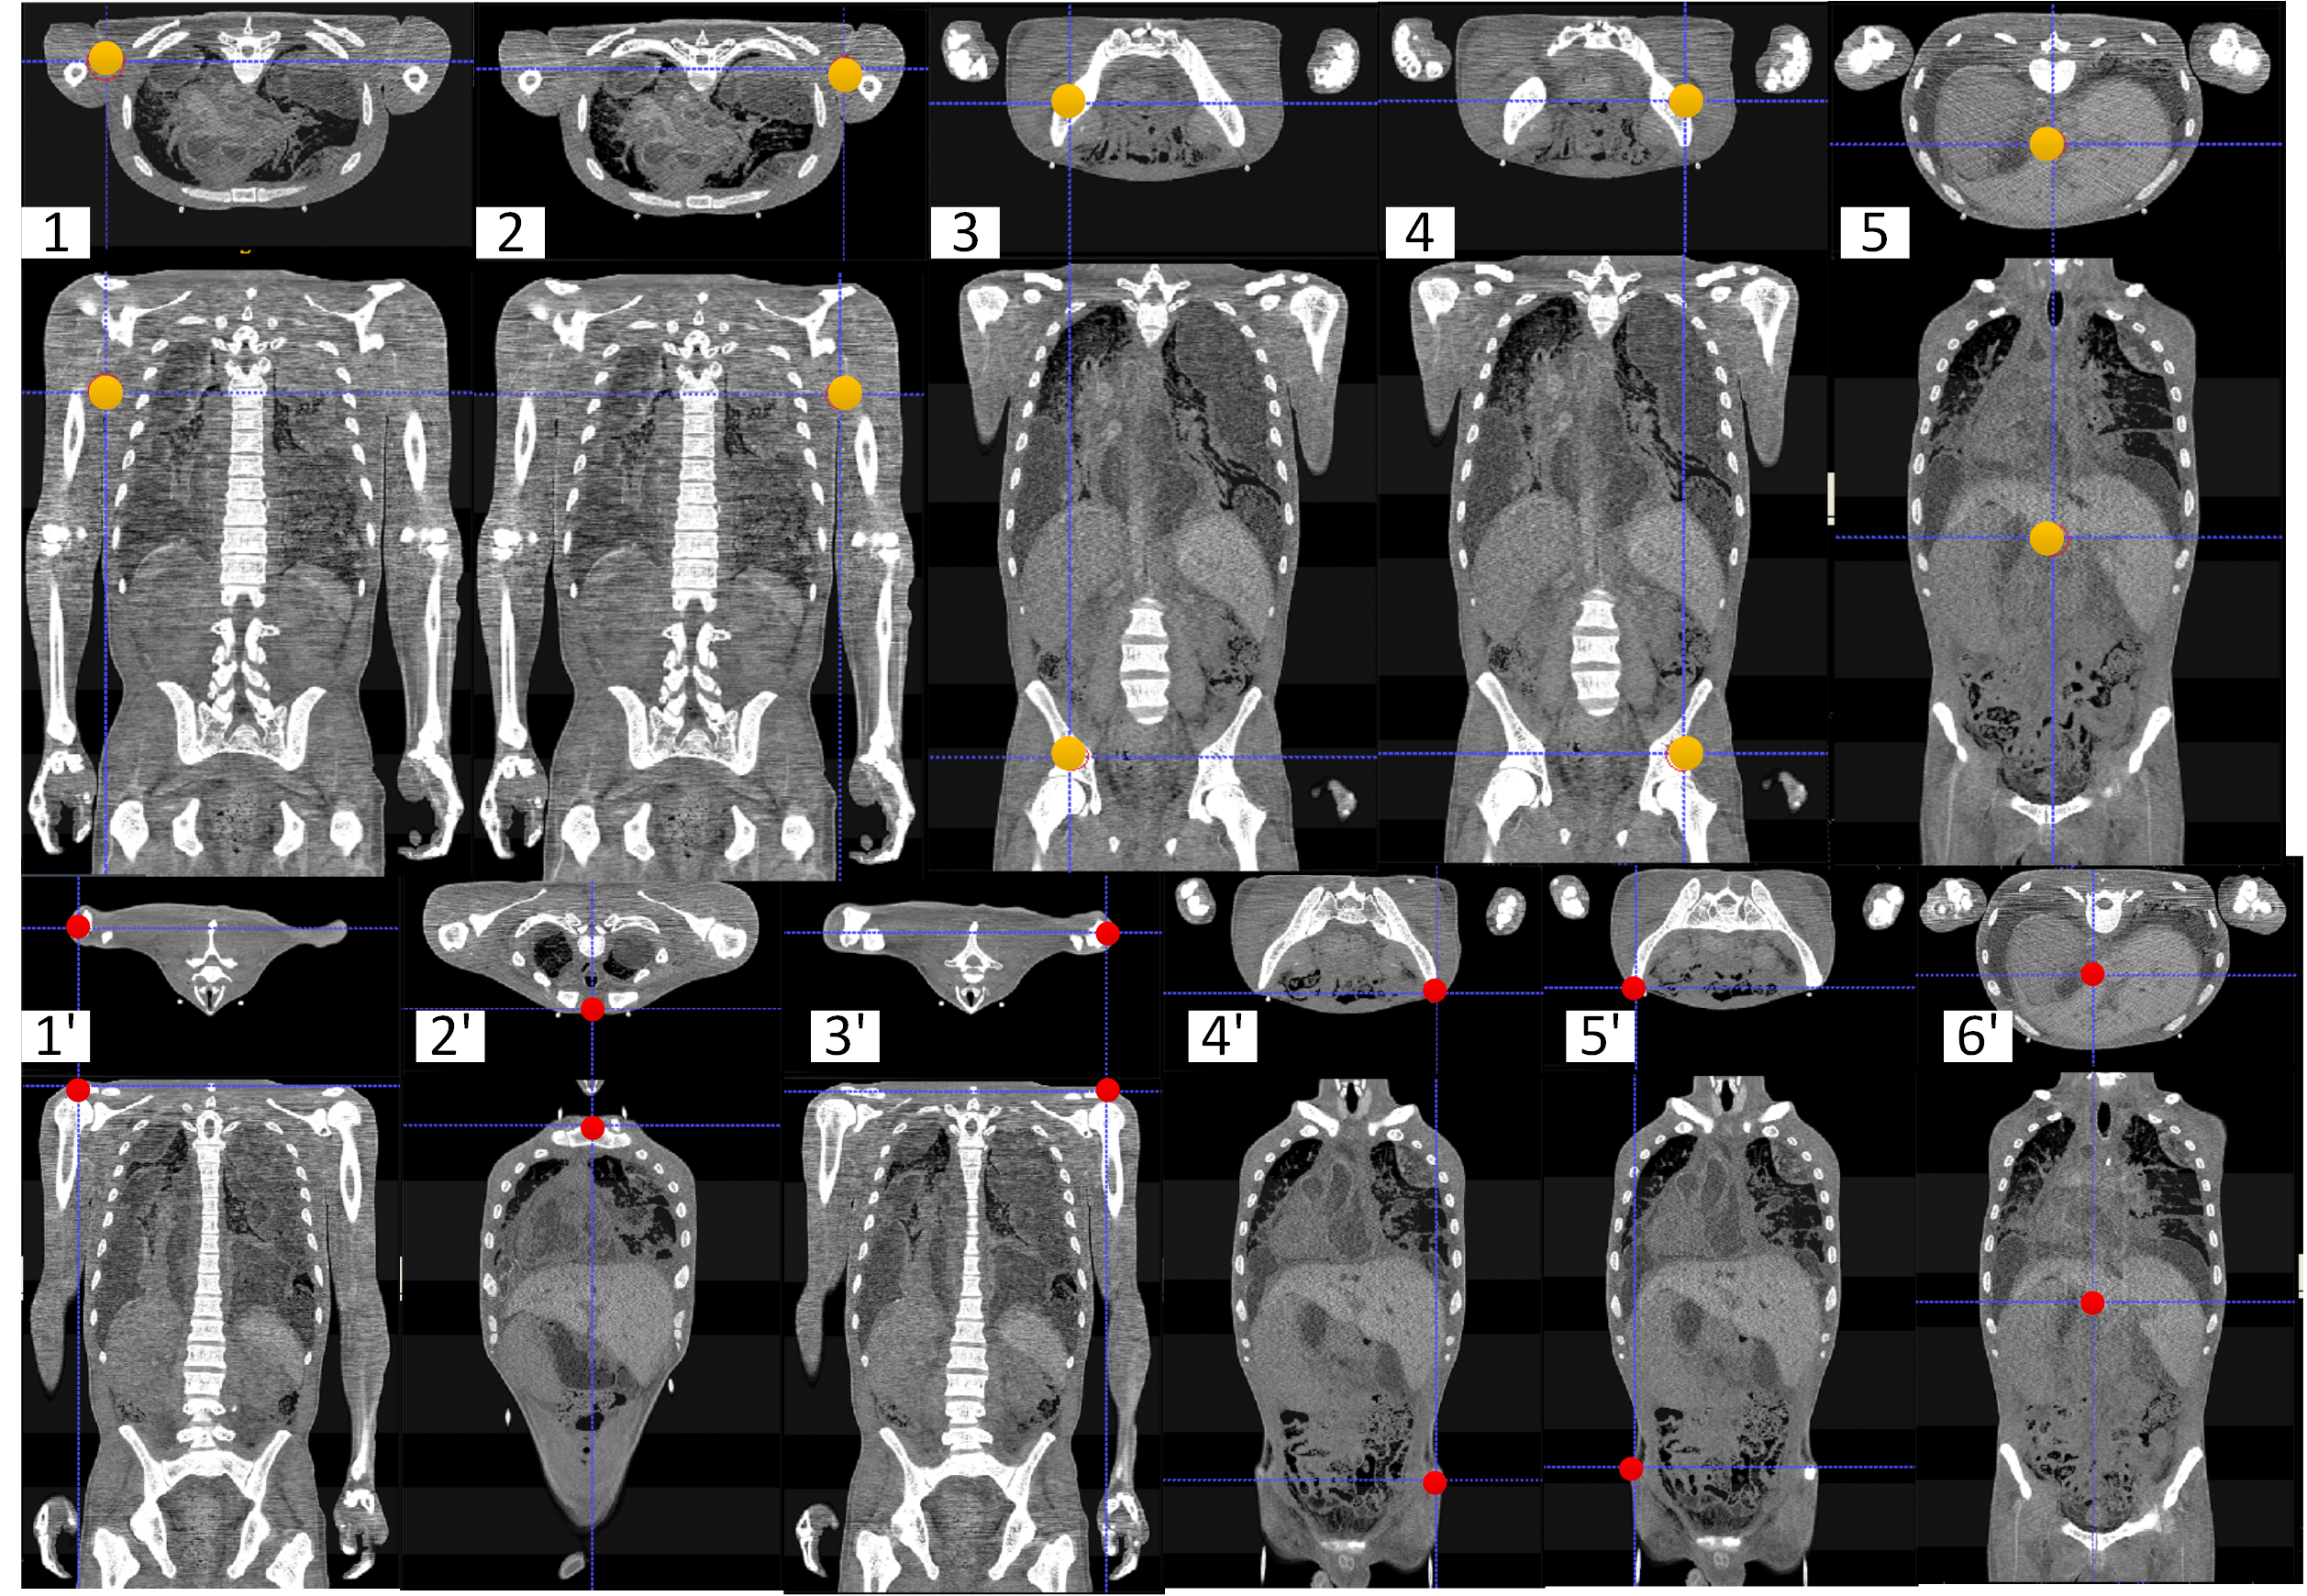
\includegraphics[height = 7cm]{figures/3-PRMM/BoneLandmarkerInCT.png}
			}
	\label{fig:3-PRMM:5points}
	\caption{(a-b) The inaccurate Kinect skeleton, in yellow, compared to the improved Kinect skeleton positions in red. (c) CT data from the Visible Human Korean showing the 5 landmarks from Kinect skeleton. (d) CT data showing correctly the 5 landmarks + interpolated torso landmark using our method.}
\end{figure} 
\subsubsection{Anatomical bone landmarkers}
Together with orthopedic surgeons, we have defined five bone landmarks that can easily be touched on the human body. These are: left and right acromion, left and right anterior superior iliac spine, and the manubrium. Subjects are positioned in front of the Kinect sensor and asked to interactively adjust the positions of five landmarks
\subsubsection{Improment of kinect skeleton}
Figure 3 shows a comparison between the traditional Kinect skeleton and its proposed improvement. The first row depicts visually the exactness of the new skeleton. The second row depicts the skeleton landmarks directly on CT data. We observe that the shoulder and anterior superior spine are inaccurate in the images. The last row depicts the improved landmark positions within CT as well. Transverse and sagittal CT slices of the visible human Korean are seen respectively in rows 2 and 3.
In Figure 3a, the following scale factors were computed for the magic mirror augmentation:

\subsubsection{Evaluation}
As an augmented reality anatomy learning application, both accuracy and system usability are very important prior to its translation in classroom. Firstly, we undertook one user study with particular users having expert anatomy knowledge to evaluate if this system is precise enough for anatomy learning. Secondly, another user study involving first year medical students took place to verify the learning potential and acceptability of our technology as a compliment to atlas textbooks in classroom.

\paragraph{Assessing the magic mirror system precision and usability}
Participants: Seven participants were included in this study (two surgeons and five final year undergraduate medical students). 
Analysis: a Likert scale was used which is a type of psychometric response scale often used in surveys and the most widely used scale in survey research. When responding to a Likert questionnaire item, respondents specify their level of agreement to a statement. The format of our 5-pt Likert was: (1) strongly disagree, (2) disagree, (3) neither agree nor disagree, (4) agree, (5) strongly agree. 
To assess the precision of our personalized magic mirror we asked the participants to interact with the system platform which integrates user-specific anatomical landmark selection. Participants were asked to provide an estimated numerical offset, if any, on how far specific bone landmarks or organs were with respect to their own body. For this, they interacted with the magic mirror window, CT data, and used their own medical knowledge and expertise for judgment. CT data was displayed in an interface depicting both transverse and sagittal planes, and participants would quantify the offsets. If needed, a ruler was provided to assist them. The anatomical targets during evaluation were defined as: the anterior superior iliac spine, manubrium, heart, and liver. Results from this exercise are shown in \tablename{\ref{tb:3-PRMM:results1}}, with offsets measured in centimeters. Results from the user study show that the precision of user-specific learning environment is on average 0.96cm.
\begin{table}
	\caption{Precision (in cm) of magic mirror system based on anatomical offsets}
	\label{tb:3-PRMM:results1}
	\scriptsize
	\begin{center}
		\begin{tabular}{p{4cm}|p{3cm}}
			Anatomy & Offset(Mean$\pm$ STDev) \\
			\hline
			anterior superior iliac spine & $0.67\pm0.52$\\
			manubrium & $0.67\pm0.75$ \\
			heart & $1.17\pm1.60$\\
			liver & $1.33\pm1.21$
		\end{tabular}
	\end{center}
\end{table}

The seven participants were then asked to judge the usability of the AR magic mirror system by responding to the following questions: (i) is the overlay accurate w.r.t human body (ii) is the user interface easy to use, (iii) is it fun to play, (iv) can it be used for medical education, and (v) would it have stronger impact for medical education learning?
The Likert scale results for the first four questions are shown in \tablename{tb:3-PRMM:results2}.
\begin{table}
	\caption{Likert scale results regarding magic mirror usability}
	\label{tb:3-PRMM:results2}
	\scriptsize
	\begin{center}
		\begin{tabular}{p{6cm}|p{3cm}}
			\space & Mean$\pm$ STDev \\
			\hline
			is the augmented reality overlay accurate w.r.t human body & $4.00\pm0.89$\\
			is the user interface easy to use & $3.67\pm1.03$ \\
			is it fun to play & $4.50\pm0.55$\\
			can it be used for medical education & $4.17\pm0.75$
		\end{tabular}
	\end{center}
\end{table}
For the last question regarding the impact of our technology, there was a unanimous response that the AR magic mirror system should be considered as a potential platform to complement existing anatomy learning tools inside anatomy classrooms. 
\subsubsection{Discussion}
The precision of our method is visually demonstrated in Figure 3c-d and \figurename{\ref{fig:3-PRMM:ResComparing}}. We observe that the acromion and anterior superior iliac spine, using the traditional Kinect skeleton, is not positioned correctly within the CT data compared to the modified Kinect skeleton version (1-2 vs. 1'-2'; 3-4 vs. 3'-4'). The orthopedic surgeons participating in our study confirmed this.
\begin{figure}
	\centering
	\includegraphics[width = \linewidth]{figures/3-PRMM/ResComparing.png}
	\label{fig:3-PRMM:ResComparing}
	\caption{Figure 4:	The magic mirror before (top) and after (bottom) the Kinect skeleton adjustment. Column 2 depicts the bottom of the rib cage being positioned correctly after skeleton correction.}
\end{figure}
Results from a user study show the impact of interactively improving the Kinect skeleton to increase precision for a better visualization of anatomy. The offsets of specific anatomical landmarks decreased significantly. The following comments were collected:
\begin{enumerate}
	\item the precision improved; making the user touch anatomical landmarks is cool since this is the way it is done in clinic…
	\item two additional landmarks easily accessible are the sternum and bottom of rib cage…
	\item make the magic mirror circle bigger for larger anatomy…
	\item voice command is a good idea but it is sensitive to the surroundings voice
	\item interactions between observers …
	\item could introduce the female CT visible human Korean…
	\item could use a healthy patient CT or other modality…
	\item could make the CT slices bigger on the screen…
\end{enumerate}

One appealing feature of the system is that with the Kinect we are using inexpensive standard hardware. In the future such a system could be made available to students or patients who have to do rehabilitation exercises at home. In addition to the full system using a large screen and a screen stand we also want to evaluate the benefit of making the system accessible to students when they are at home and at any time. We want to do this for two different reasons. First, there is a trend toward competency-based education in medicine. Instead of defining a curriculum, learning outcomes are defined. Students have to fulfill these learning outcomes. The advantage of competency-based education is that all students will have the same competency in the end. A student who is less skilled has to take more time to learn than a student who already has good skills. One requirement for this is that the students have to be able to educate themselves until they reach the required competency. We plan to use the AR magic mirror system both to allow them to do training and to test whether a learning outcome has been met. The magic mirror has to be made easily available to them so that they can use it for training at any time. The second reason to develop a distributed system which can easily be used by students is to collect user statistics.

Many medical education systems are web-based and allow accessing them from every computer. However current systems do not use high-end visualization and input devices like the Kinect. In the future when technologies like HTML5 and WebGL have matured it can be imagined that a system like the magic mirror could be implemented using web technology such that it can run on any computer. However, at the moment the use of web technology would be a significant limitation. We are using very large datasets, high-end visualization, GPU computing and gesture-based interaction.

It was originally suggested to us that our system would have much more of an impact for medical education learning if it were to be translated today in medical schools and anatomy classrooms. As such, with the help of our co-author and anatomy professor, we deliver the improved AR magic mirror to two anatomy classes within the Anatomy Department of the Ludwig Maximilian University (LMU) Medical School, Munich, Germany. The anatomy professors made it clear that the AR magic mirror system is exciting, but has to go beyond state-of-the-art technology to be truly useful for education. Our participants stressed the importance of visualization of anatomy that can change dynamically resulting from the actions of the user moving the body, and also for visualization of muscles. Furthermore, more advanced user interactions like the use of gaming elements would be required to make the use of the system for learning tasks more interesting.
% !TEX root = ../thesis-example.tex

%todo: Make the user believe the virtual element is a part of his or her own body. (Organ game and the Muscle learning)
\section{Interactive mixed reality and serious gaming} \label{sec:3-PPMM:IMR}
%Personalized natural interaction \& gaming
Knowledge is a process of understanding by connecting. Although we can learn by reading and watching, the learner always needs to encode the knowledge by themselves, rather than simply receive what is shown. This is one of the reasons that interacting with the mixed reality system can be a powerful learning tool - we do not only get the benefit of the AR view, but also receive immediate feedback. These interactions are often useful in creating the `WoW' moment -- the joining of medical knowledge with a learner's own body and movement.
In Section \ref{sec:3-PPMM:Registration}, user's personal information is collected to improve the perception of the medical information.
Here, we implement several applications by integrating exciting user-interaction and gaming concepts within the proposed Magic Mirror framework.
 
%Two kinds: user motivate interaction (user's movement trigger the changing) and scenario interaction (AR view change according to the presetting), combine two kinds together. 
In this section, a new interaction with anatomy is firstly developed for learning in the MR Magic Mirror framework. It is demonstrated by two new modules using the organ atlas and an education game.
Then, we focus on the muscles of one human arm to find out a solution for muscle learning. 
%Thirdly, the system is extended to visualize the basic function of the human skeleton and muscle system, and it highlights the active muscles and implement a labeling system based on the interaction, creating a personalized MR muscle learning environment. 
Finally, serious gaming for education and rehabilitation is discussed and a knee rehabilitation demo is developed. 

\subsection{Interaction for anatomy learning} \label{sec:3-IMR:anatomyLearning}
Basic knowledge of human anatomy is also considered common knowledge that is taught at various levels of school education. To improve the conventional book-based methods for anatomical education, we have investigated the suitability of an MR system using a Magic Mirror metaphor for this task.
With the existing platform, we develop an interactive educational application consisting of an organ atlas and a complementary organ learning game, leveraging the benefits of self-referential learning and motivation through game challenges.
The organ atlas is a good way of imparting anatomical knowledge on the users, allowing them to explore their body without any instructor or supervisor.  The education game is developed taking advantage of the new interaction method with the anatomy. 

%To achieve intuitive usability, we investigate different user interaction methods for organ selection in a self-referential system using augmented reality, providing methods for unique selection as well as coarse, non-unique selection.
\subsubsection{Motivation and objective}
In the original Magic Mirror MR learning environment, the users can see themselves on the screen like in a mirror with medical information augmented onto their body and a feeling of ``looking inside'' the human body. The user can also relocate the see-through window and interact with slices as described in Section \ref{sec:3:MMCInteraction}, but the user cannot directly interact with the organ anatomy. Here, we try to expand the existing framework to be used as an alternative and entertaining way to learn human anatomy. An educational application is developed to allow the user to explore their body and learn about spatial relations, visual appearance and function of the organs.
As atlas and text are still the main learning methodologies, we also want to merge these traditional information into the MR learning environment. 
%An organ learning game to provide an entertaining way to learn anatomy is also presented in section \ref{sec:3-IMR:gaming}. This game is based on the knowledge presented in the atlas and leverages augmented reality and motivation through game challenges to improve the learning performance of the user. 
%To achieve this goal, we examine different interaction metaphors and their suitability for the tasks presented.

The objective is to implement an interactive anatomy atlas that also focuses on the inner organs of the torso. The user can explore these organs and read additional information on each of the visualized organs. The work is separated into two different parts: general interaction methods performing all kinds of basic operations not specific to any application and the logic implementation of the actual application, and realizing the organ atlas application.
The general interaction methods are designed to be one part of the Magic mirror AR view, as shown in \figurename{\ref{fig:3-MMC:systemFramework}}, and provide easy access to implement custom application logic, making it easier to experiment with new ideas based on the Magic Mirror framework.

\paragraph{Challenges of interaction}
The main challenging issue is the interaction method with the organ model. We need a method to reliably detect which organ the user has selected while leveraging the mirror analogy as far as possible. The most intuitive and direct way would be to use a virtual hand technique to directly select the organs \cite{Ha2010a}. However, this is bound to fail for two reasons.
First and most obviously, it is not possible for the user to put a hand into their body and directly touch the organ. Only the approximate region in front of the organ is reachable, but it is not accurate in many cases as it is not really possible to detect reliably which organ the user points to. 
Especially in the abdominal area many organs are fit very tightly together in one place, making it very hard to distinguish between two organs.
Secondly, the tracking capabilities of the current version of Kinect sensor are not robust. The only thing suitable for selection is the position of the hands. 
Untrained users usually use their fingers when asked to indicate a point.
Neither orientation of the hand nor information about the fingers is available when the hand is put on their body. 
This makes it even harder to develop a suitable, intuitive interface. 

\subsubsection{General interaction methods}
%The investigation of possible interaction methods forms an important part of this work. 
Since conventional point-and-click selection methods are only of limited use for self-referential selection in MR environments, we have developed new methods better suited for our scenario: (i) One is driven by a two-handed interaction method to allow the user to select the region of interest with one hand and using the other hand to select a specific organ; (ii) the other uses a single-handed approach where the user indicates the organ directly by touching the specific region of their torso \cite{weiss2013}. 

\paragraph{Organ Explosion}
%In the AR learning environment, organ selection is a challenging task as some organs hide behind others. The user cannot directly position their hand into their bodies and to select the organ of choice. 
Our approach to overcome the selection challenge is a technique that we have called ``Organ Explosion'' effect (see \figurename{\ref{fig:3-IMR:organExplosion}}).
This technique is inspired by exploded view drawings known from engineering, where the goal is to depict how mechanical parts need to be assembled. Usually they are drawn with the innermost part at the center while the other parts are moved some fixed distance outwards to display all parts of the assembly that would otherwise be hidden.
We use the same basic idea in our interaction technique by implementing a two-handed interaction method. Using the left hand, the user is able to set the focus height for the region they are interested in. Organs at approximately the same height are then projected outwards. Because we use a spherical projection with the center position at the height of the hand, but at a point behind the body, the organs are moved outwards creating the illusion of seeing them ``fly out'' in front of the body. Lines are drawn to indicate the original position of the organs. After separating the organs from each other, it is easy for the user to select the organ of interest using the other hand.
This way we are able to separate the organs close together since organs at different angles to the projection point are projected into different regions. We scale the magnitude of the displacement down with the distance between hand and body to allow the user to see the organs in their original arrangement but still enable the user to ``zoom in'' for detail and selection. \figurename{\ref{fig:3-IMR:organExplosion:b}} depicts how this technique looks in practice.
Once we are able to separate the organs from each other, it is easy to perform selection by checking the intersection between the hand and the organ. Another functionality of the organ explosion effect is allowing the user to rotate and observe the 3D organ models and perceive the spatial relationship between them.
\begin{figure}
	\subfloat[Front View] {\label{fig:3-IMR:organExplosion:a} 
		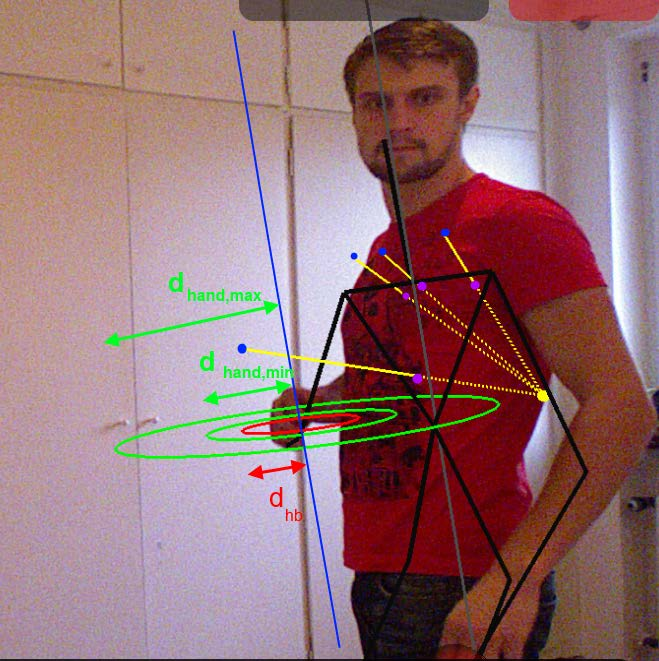
\includegraphics[height= 7cm]{figures/3-IMR/organExplosion2}}
	\subfloat[Side View] {\label{fig:3-IMR:organExplosion:b} 
		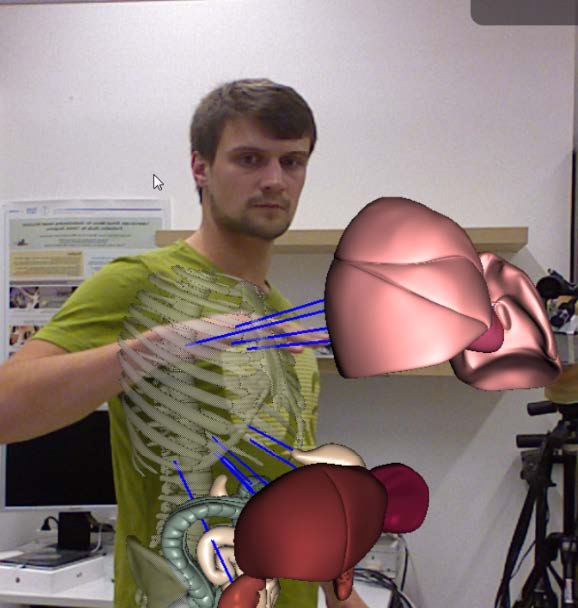
\includegraphics[height= 7cm]{figures/3-IMR/organExplosion1}}
	\caption[Organ Explosion]{Left: Quantities involved in the calculation of the position offsets for the technique (organs not displayed). In this image, four organs are displaced. Purple dots are original organ positions, blue dots displaced organ positions and the Yellow dots signify the spherical projection. Right: Screenshot of the explosion technique.}
	\label{fig:3-IMR:organExplosion}
\end{figure}
The interaction methods we developed are not necessarily limited to self-referenced selection and manipulation. In general cases, they are suitable for scenarios where many possible items are densely packed and a user wants to select a single or multiple items in an augmented or mixed reality environment. The large number of possible modifications to the methods make them difficult to configure, but the general idea should be applicable to many other cases.

\paragraph{Interaction test for selection}
Intersection detection between different 3D objects is a built-in functionality in many rendering libraries. A virtual predefined sphere or box can be attached to the control hand of the current user and defined as the hand object, and the selection function is triggered when the intersection between the hand object and the organ models occurs. 
For performance reasons, we only use bounding-box intersection tests and skip the narrow phase, treating intersecting bounding-boxes as intersections between geometry. This obviously reduces the accuracy of bounding box tests. This coarse intersection check is better not only in performance, but also from a usability perspective. Intersection tests in our applications are used for checking intersections of the hands with organs. Due to the inaccurate tracking of the hands by Kinect, this actually works quite well when just verifying for ``roughly" intersecting pairs.
%To further improve performance, we introduce an explicit vector that describes objects that are actually interested in intersections with other objects. The assumption is that general intersections, for example between two organs, are not of interest, while intersections with special objects like a sphere attached to the user's hand are interesting and important. Once an ``interesting" intersection has been determined between a pair of objects, the first object gets added to the intersecting objects list of the second and vice-versa. This list can then be used and analyzed in the behavior implementation to perform reactions to the collisions. For convenience reasons, there are two vectors configured to be attached to the left and right hand. They can be added to the framework if required and reconfigured by the application implementation.

\subsubsection{Organ atlas application}
An organ atlas is usually a collection of visual representations of organs or specific organ systems, annotated with names and physiological information.
We reproduced a version of this concept using the Magic Mirror framework with personalized interaction. The main educational goal of this application is to allow the user to explore the organs of their body and learn about the shape, position, function and 3D spatial relations to the other organs.
We approach this goal by augmenting all available organs onto a user's body and letting the user select the one they are interested in via an ``Organ Explosion'' effect. Once the user has selected an organ, the application displays textual information about the organ. This information includes the latin and/or greek names as well as a description of the basic function of the organ. During the selection process, the knowledge about the spatial position is also obtained. An example of what the application looks like in action and when finished is shown in \figurename{\ref{fig:3-IMR:OrganAtlas}}. The organ atlas offers an interesting new way to explore the human anatomy. However, the described methods offer much room for experiments and improvement. The organ learning application in its current prototype version already provides a fun experience, but it lacks the content to be distributed as a full game. This could easily be changed by adding more game modes for other organ systems, multi-player modes or other elements commonly found in computer games.
\begin{figure}
\centering
\subfloat [In action] {\label{fig:3-IMR:OrganAtlas:a} 
	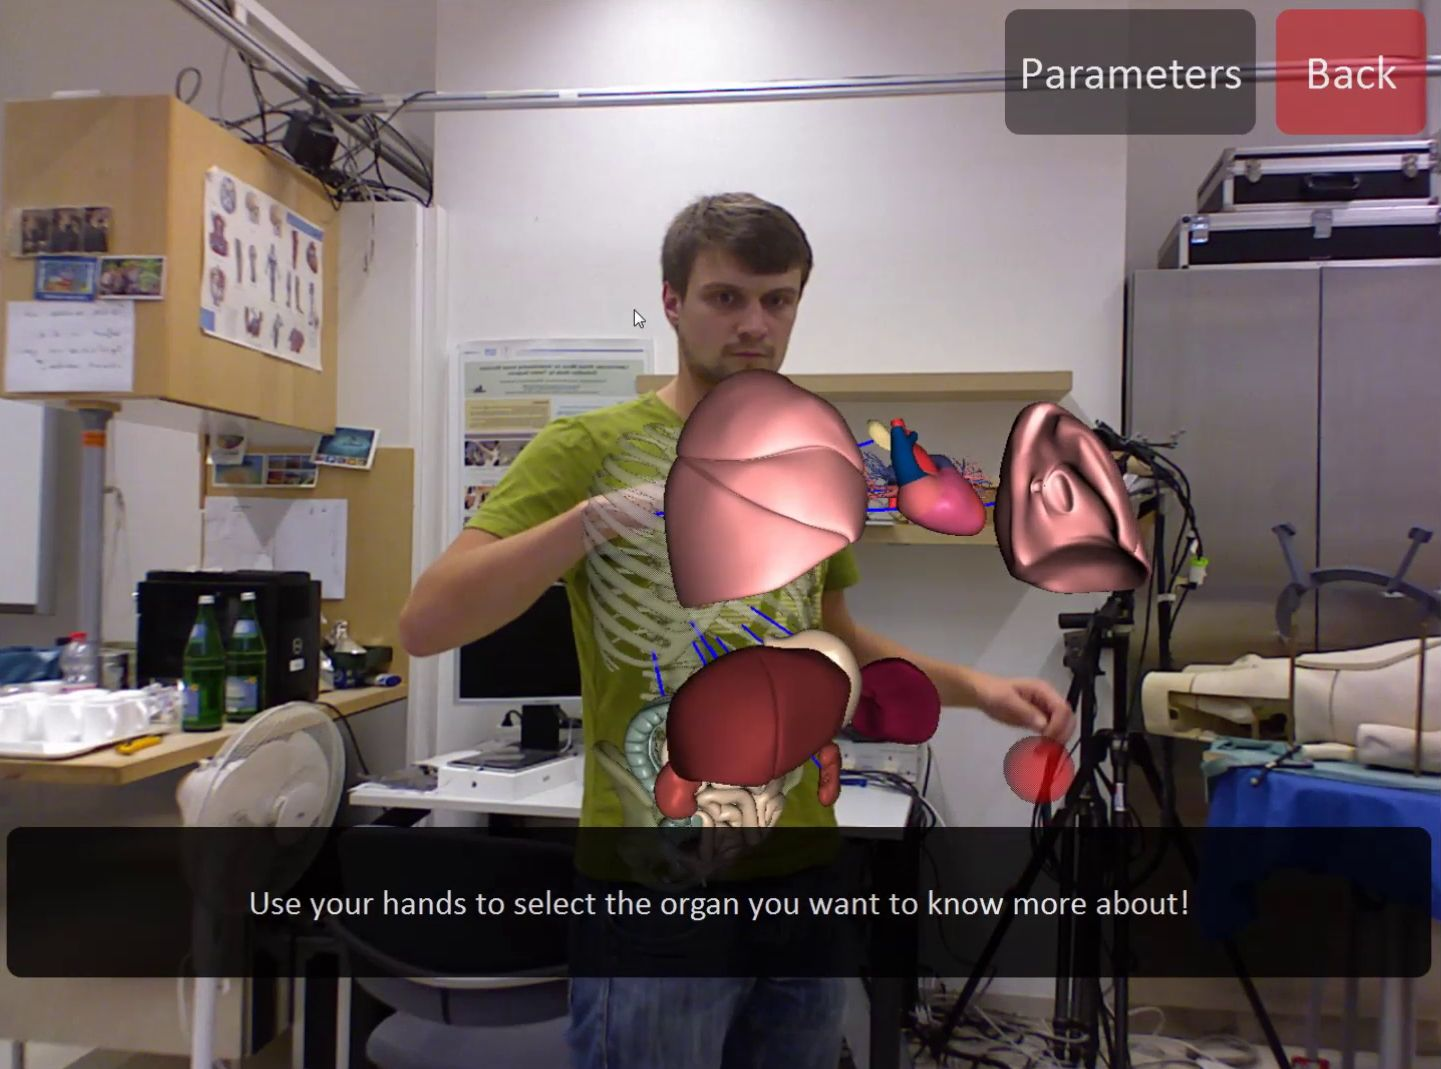
\includegraphics[width = 0.5\linewidth]{figures/3-IMR/FrontViewOrganExplosion}}
\subfloat [Finished] {\label{fig:3-IMR:OrganAtlas:b} 
	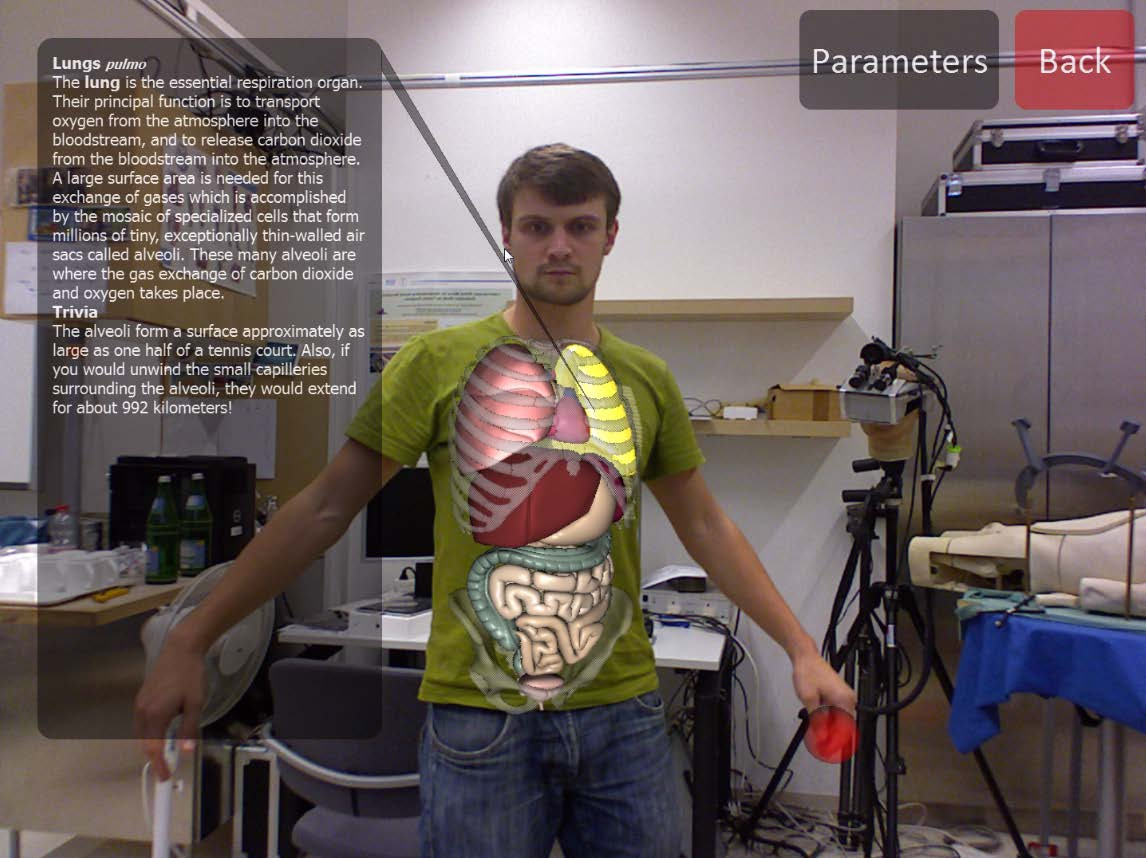
\includegraphics[width = 0.5\linewidth]{figures/3-IMR/OrganAtlas}}
\caption{Organ Atlas implementation. Lungs are selected and the infobox shows textbook knowledge about them.}
\label{fig:3-IMR:OrganAtlas}
\end{figure}
%The optimal choice of all parameter values is a very delicate matter that has not been explored fully in this work. The values chosen on an empirical basis seem ``good enough'' to at least show that the methods work reasonably well to be used productively. To determine a better parameter, one should conduct a separate study and compare the performance results to generate the parameter settings according to the personal information of the untrained users. Also, the different variations of the methods offer even more room for fine-tuning the effectiveness of this method. 

\subsubsection{Organ game}
A serious game is developed for general users to learn basic anatomy called ``Whack an Organ''. The game is based on the idea of the classic arcade games at carnivals, ``Whack-a-Mole''. We implement a similar game idea using the proposed interaction methods. It is a combination of Whack-a-Mole and classical quiz games. Questions regarding human anatomy are shown to the user, and the answers are always one organ or organ system. 
This knowledge will serve as a basis for the game. This game works in a quiz-show like manner where the user has to answer questions by indicating the right positions of the organs.
To answer the question, the user has to point to the location of the organ directly on their body. 
The game then decides if the location is correct and awards points if so. Questions can come from different question sets with varying difficulty, ranging from simple location questions: \textit{where is the liver?}, to more complex knowledge questions: \textit{which organ is infected if you have Hepatitis?}.
Still, the questions have to have a concrete organ as an answer, limiting the possible range of anatomy-related questions. At the end of a question round, the achieved points are shown to provide some feedback on the performance of the player.
We hope to provide an experience that is both entertaining and fun to persons of all ages.
%but due to the simplicity of the questions and detail of information displayed, for our first version, the target group can be considered children and teenagers where the common knowledge about human anatomy is not as present as with more adult persons.

\paragraph{Organ bounding box selection}
A direct approach is to do the bounding box interaction test between all the organs and a virtual box, which is attached to the hand. 
Once an intersection has been detected, we use a timeout to allow the user to position the hand correctly. Once the timeout has run out, we collect all organs that are currently intersected as our selection set (see \figurename{\ref{fig:3-IMR:organGamingBoundingBoxSelection:a}}).
We increase the length of the virtual box in negative Z direction (towards the back of the body) to be as long as the user's torso width. This is because some organs like the kidneys are located in the dorsal area of the torso and they still have to intersect with the box when the player touches the front.

\begin{figure}[htb]
	\centering
	\subfloat[Bounding box]{ \label{fig:3-IMR:organGamingBoundingBoxSelection:a}
		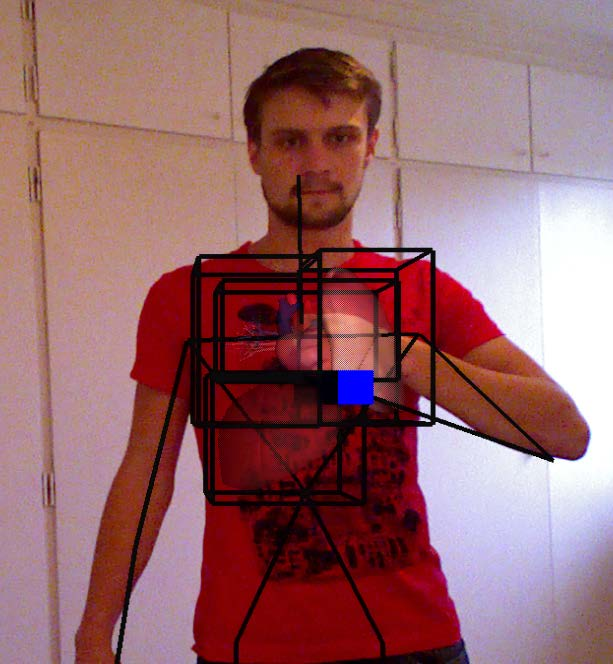
\includegraphics[height=0.45\linewidth]{figures/3-IMR/organGamingBoundingBoxSelection}
	}
	\subfloat[Sphere interaction]{ \label{fig:3-IMR:organGamingBoundingBoxSelection:b}
		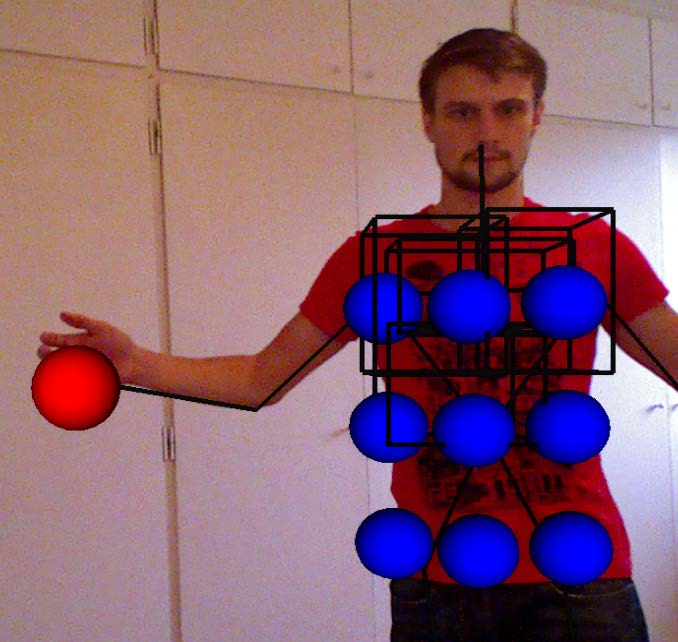
\includegraphics[height=0.45\linewidth]{figures/3-IMR/organGamingSphereSelection}
	}
	\caption{Debug visualization output of the two selection techniques. (a) Organ Bounding Box Selection: Blue box is intersector box of the left hand. (b) Sphere Selection: Blue spheres are the selection regions, red sphere is the intersector of the right hand.}
	\label{fig:3-IMR:organGamingBoundingBoxSelection}
\end{figure}
\paragraph{Sphere intersection}
Another solution is inspired by taking the Whack-a-Mole concept one step further. We define a fixed number of selection regions attached to the body of the user. Those regions are labeled by virtual spheres or boxes, which are attached to the front of the trunk and are separated far enough to allow for an unambiguous selection. We compute the closest sphere for every organ at the initialization in advance. These spheres act as a proxy for the actual organs, so the user only has to select the sphere closest to the organ in question. 
We detect the selection of the spheres via bounding box intersection.
Once we have detected the selection, we check if the correct organ(s) are associated with the selected sphere and determine the correctness of the answer. The number of spheres can be varied and several spheres can be associated with one organ. 
% that are possible for selection. 
%Increasing the number of spheres has a number of effects on the method. At a first glance, the accuracy gets better: The more selection spheres there are, the closer an associated sphere is to the actual center of the organ. On the other hand, it gets considerably harder to select the correct sphere the smaller they get. Not only is it problematic when the sphere radius gets smaller than the organ size, but also the tracking stability of NiTE suffers when the user holds his hand in front of the body, resulting in selections the user didn't intend just because the skeleton tracking was wrong. Practical tests suggested that a grid of 3x3 or 3x4 spheres is the best choice for this method. 
%This could solve the problems with tracking inaccuracy and also help increase the number of spheres. However, this requires a more sophisticated algorithm to determine which spheres are associated to which organs.
%Finally, a radical modification is that one virtual box of the approximate size of the torso is added as a dummy to detect when the player has touched the body. Once this touch has been detected, we can determine the selection by including all organs at a certain radius from the hand in the selection set. 

\paragraph{Implementation}
The implementation of the game is rather straightforward based on the application framework. We first load an appropriate question set from the hard drive. Question sets consist of a list of questions together with a set of correct answers for each question. The answers are given as a list of organ names and then we calculate the closest sphere if needed.
After setting up the basic game state variables like the current question and counters for correct/wrong answers, we proceed to set up a default behavior for all organs. This behavior keeps an organ invisible for most of the time. Only when the user has selected an answer and the organ is in the set of correct answers for the current question, it is made visible for a short time (see \figurename{\ref{fig:3-IMR:organGaming}}). At the time, it flashes either red or green, depending on whether the answer is right or wrong.
%For the first selection method, we now set up the intersection spheres on a regular grid in body space. After we have determined the positions of the sphere centers, we perform the calculation for the nearest spheres for each organ. The spheres and the results of this calculation are stored as static variables to allow the hand behavior access to this data.
\begin{figure}
	\centering
	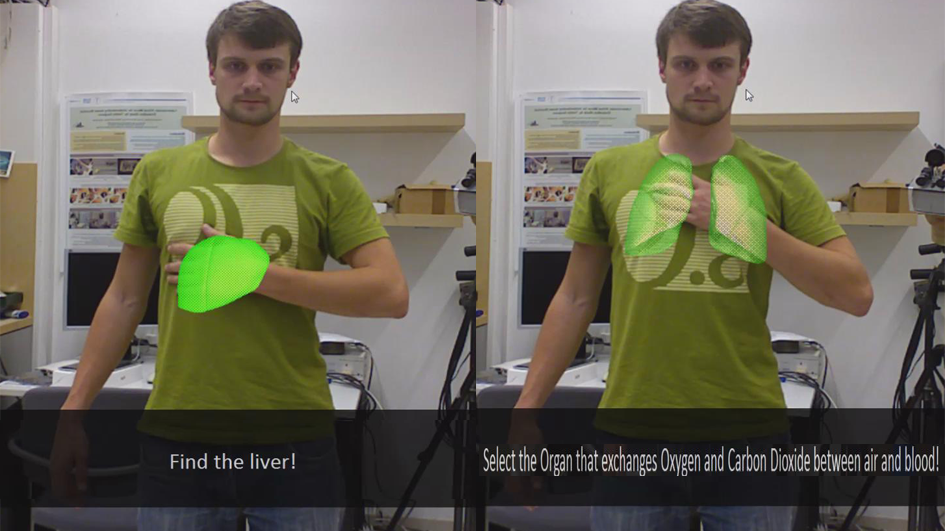
\includegraphics[width=0.7\linewidth]{figures/3-IMR/organGaming}
	\caption{Whack an Organ. This game works in a quiz-show like manner where the user has to answer questions by indicating the right positions of the organs.}
	\label{fig:3-IMR:organGaming}
\end{figure}
%The behavior functions for left and right hand are identical in this game to allow the user to select answers with both hands.
%For the sphere-based method we test the intersection between the hand object and spheres. In the behavior, we then determine whether the hand is currently intersecting a sphere and if so, decrease our timeout. If the timeout has run out, we determine the selection set by using all the associated organs of the selected sphere.
%If we use the bounding box method, we just check if an intersection between hand object and organs has been detected to decrease our timeout. When it has timed out, we use all intersecting organs as the selection set.
Once a selection set is determined, the application checks whether it contains a correct answer. According to this, a short feedback is displayed and the counter for correct or wrong answers is modified accordingly. Afterwards the next question is presented if there are any questions left. One important thing for usability is to prevent the system from accepting the current position as an answer for the next question as well, because the hand is still intersecting and the timer has run out. We chose to solve this by setting a flag that prevents accepting new answers. This flag is only cleared when the user has moved the hand completely away from the body.

The organ learning game implemented as a proof of concept offers an engaging and fun way to learn about the human anatomy. The intuitive concept of indicating the organs on the players' own body should offer an increased learning intention. 
We hope to extend the system by providing different difficulty levels to make it more interesting for a larger target group.
 
\subsection{Interactive muscle learning}
Muscle learning is a very important and difficult topic for all the medical students as it is a complex system and several muscles are active to perform one motion.
Functions of the muscle are not easy to learn as it is very difficult to observe certain motions in humans.
Bones of the skeleton system are rigid objects and are controlled by muscles via attachment points. From any outside tracking systems, the poses of the bone can be calculated.
The main objective of the application is to enable the user to acquire knowledge about the muscles of the arm %(see \figurename{\ref{fig:3-IMR:armAnatomy}}) 
by directly connecting all the virtual information with their own arm movement. 
Based on the Magic Mirror framework, the non-physical visual effect is the activities of the muscles and the bones. A virtual model of an arm is rendered according to the real arm movement and the AR view is generated.
After discussion with our medical partners, the main muscles of one arm related to four basic movements \textit{flexion}, \textit{extension}, \textit{pronation}, and \textit{supination} are defined. The learning targets are the main muscles, which expand and contract during the completion of the above movements (see \tablename{\ref{tb:3-IMR:motionMuscles}}). 
%\begin{figure}
%	\centering
%	\subfloat{
%		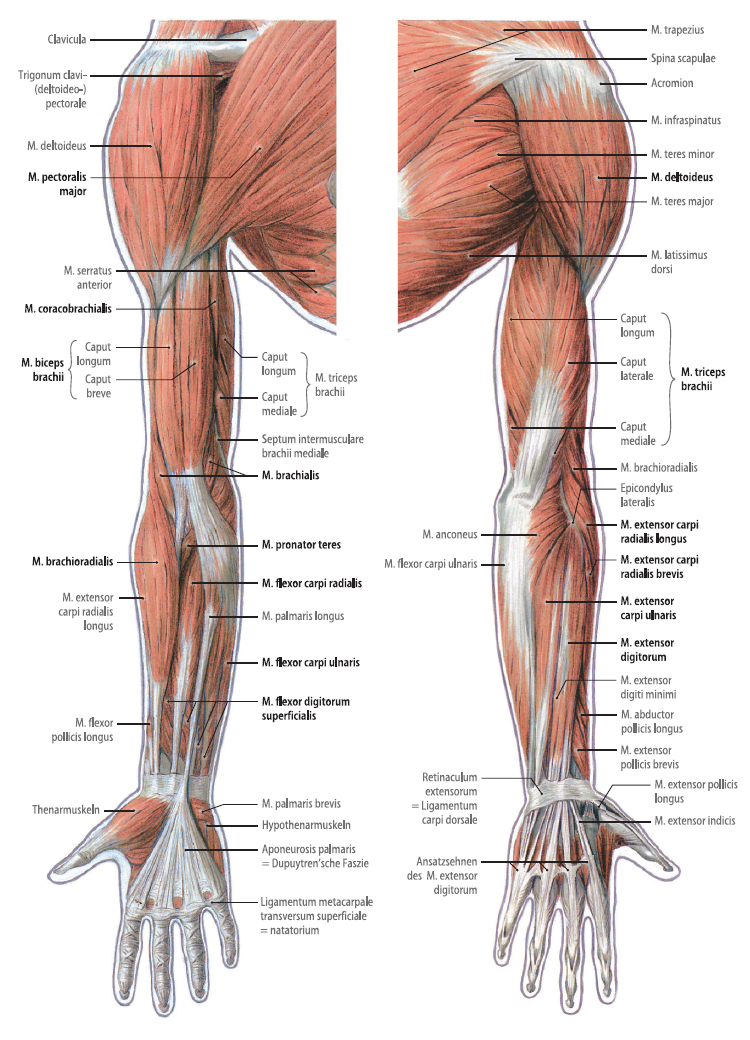
\includegraphics[width=0.35\linewidth]{figures/3-IMR/armAnatomy1}
%	}
%	\subfloat{
%		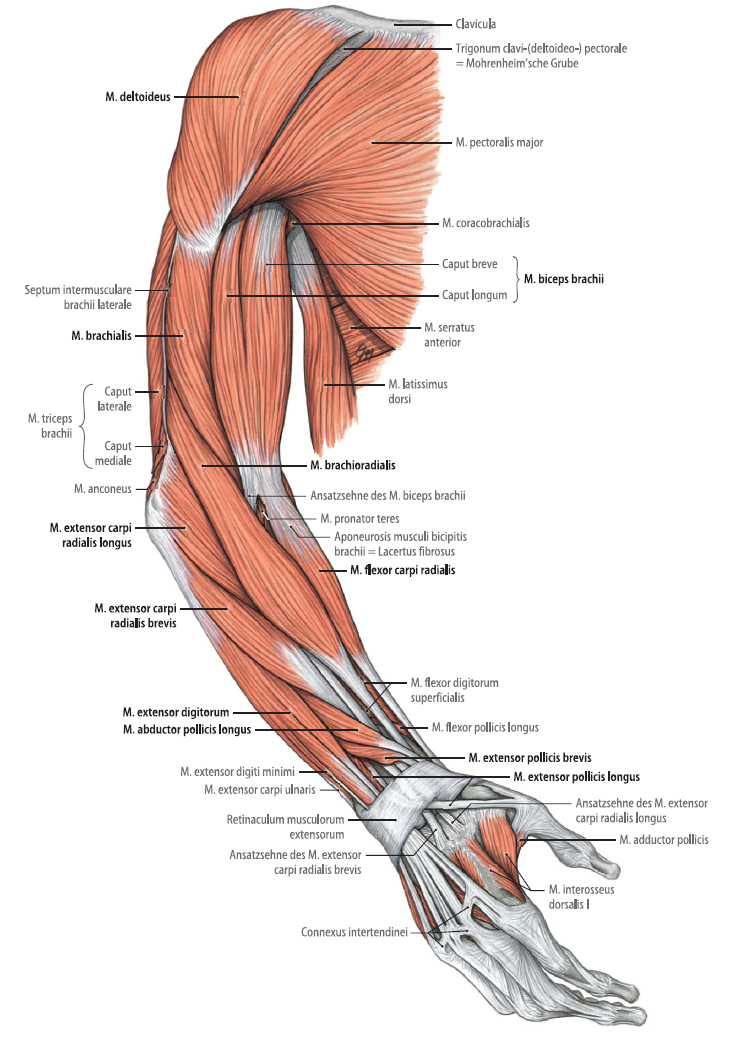
\includegraphics[width=0.35\linewidth]{figures/3-IMR/armAnatomy2}
%	}
%	\caption{Anatomy of the arm}
%	\label{fig:3-IMR:armAnatomy}
%\end{figure}
\begin{table}
	\caption[Muscles involved]{The selected motion of one arm and the corresponding main muscles}
	\centering
	\label{tb:3-IMR:motionMuscles}
	\scriptsize
	\begin{center}
		\begin{tabular}{|c|c|}
			\hline
			Motion & Muscles \\
			\hline
			\multirow{2}{*}{Flexion} & M.biceps brachii \\
			& M.brachialis \\
			\hline
			\multirow{2}{*}{Extension} & M.triceps brachii \\
			& M.anconeus \\
			\hline
			\multirow{2}{*}{Pronation} & M.pronator teres \\
			& M.pronator quadratus \\
			\hline
			Supination &M.supinator \\
			\hline
		\end{tabular}
	\end{center}
\end{table}

\subsubsection{Application design}
The application contains an AR view, which shows the color image from the Kinect with the augmented virtual arm. This view acts as the Magic Mirror effect and helps the user to map all the activities of the bones and muscles onto their own arm. There is another VR view which is also synchronized with the real arm motion. The virtual view concentrates on the upper or lower arm, showing the details of the muscle model. To preserve the connection between the user and the virtual arm, the AR-view is shown on the left side of the screen after the user is calibrated (see \figurename{\ref{fig:3-IMR:MuscleLearningSelfControlCamera}}). 
The learning procedure include `muscle-oriented', the muscle is displayed one by one, and `motion-oriented', the user performs the target motions and only the muscles related the current motion is shown. 
The system also allows the user to observe the muscle model from different viewpoints to learn the spatial information and the learning flow is flexibly scripted \cite{Jutzi2015}. 

\paragraph{Dynamic muscle model}
%\paragraph{Skeleton information}
%The position and rotation of the skeleton model are defined in a strict hierarchical order, starting with the spine. The position data from Kinect skeleton stream is in the world coordinate system. To animate the arm model, the relative orientations have to be calculated based on the position of the joints. Only the spine position is directly set as the root's position in the AR view. 
%The lower arm is treated separately to the other bone chains. Each hand's orientation is defined using the vectors from the wrist to the tip of the hand, and from the wrist to the thumb. Additionally, to be able to follow the shoulder's full range of movement, the upper arm uses the direction of the lower arm to define its orientation along its length axis.
%In order to adjust to differences in the users' height and physique, the individual bones are scaled whenever a new user is selected. For each node, the distance between its position and the position of the next node in the chain is used to calculate the scaling factor. To increase the accuracy, that distance is averaged over multiple frames before calculating the scaling.
%That makes it possible to use the absolute rotations from the Kinect with a hierarchical skeleton that would usually prefer relative orientations. With hierarchical skeletons, the position data from Kinect is only used for nodes without parent, the remaining nodes are positioned through their parent's rotation and scaling, thus only the root's position is set directly in a complete skeleton. This behavior can be disabled to always use the absolute positions even with hierarchical skeletons. As with the positions, there are two modes to rotate the nodes to choose from. The first one uses the rotation from Kinect, modified according to the axis-settings in the skeleton. The second uses the position data to calculate the orientation via Look-Rotation to align one axis with a \textit{lookAt-target}. To define the orientation along this look-direction, a second vector is supplied. Unity offers a function to create a Look-Rotation, but this always aligns the objects z-axis with the target and uses its local y-axis to define the axial rotation, so a more flexible version of this function was implemented.
%\begin{figure}
%\centering
%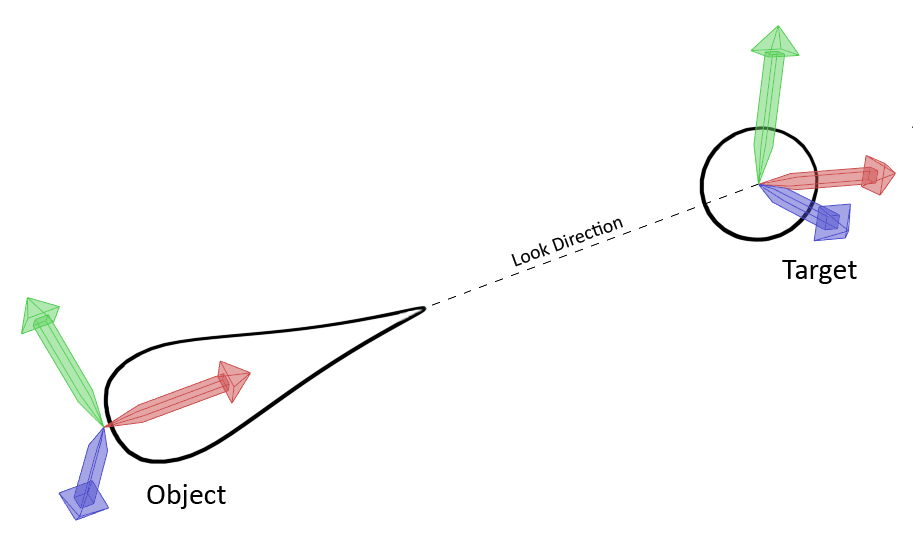
\includegraphics[width=0.7\linewidth]{figures/3-IMR/LookingRotation}
%\caption{Look-Rotation along the object's local x-axis (red)}
%\label{fig:3-IMR:LookingRotation}
%\end{figure}
%\paragraph{Muscles and Bones}
An anatomical model of a human male body from ANATOMIUM 3D\footnote{\url{http://www.anatomium.com/}} is employed as the virtual arm model.
%This model includes all the anatomy, such as skin, muscles, bones, blood vessels and so on (see \figurename{\ref{fig:3-IMR:humanModel}}).
%\begin{figure}[htb]
%	\centering
%	\subfloat[Skin]{\label{fig:3-IMR:humanModel:a}
%		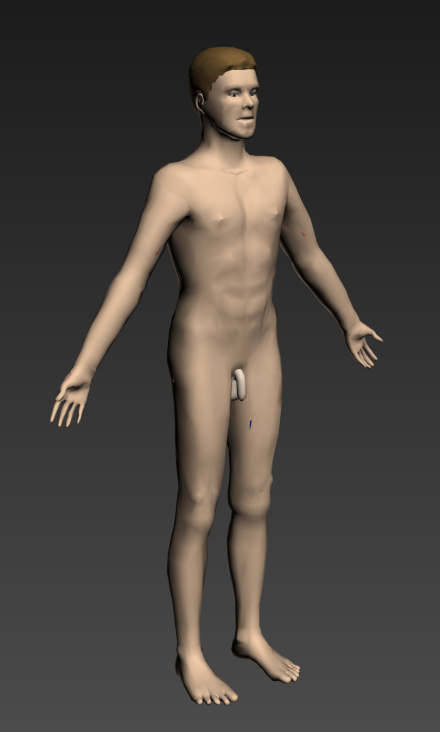
\includegraphics[width=0.32\linewidth]{figures/3-IMR/muscleSkin}}
%	\subfloat[Muscles]{\label{fig:3-IMR:humanModel:b}
%		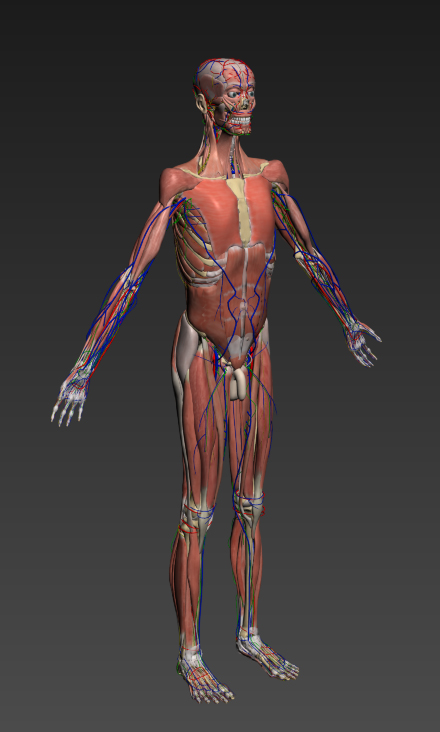
\includegraphics[width=0.32\linewidth]{figures/3-IMR/muscleMuscles}}
%	\subfloat[Skeleton]{\label{fig:3-IMR:humanModel:c}
%		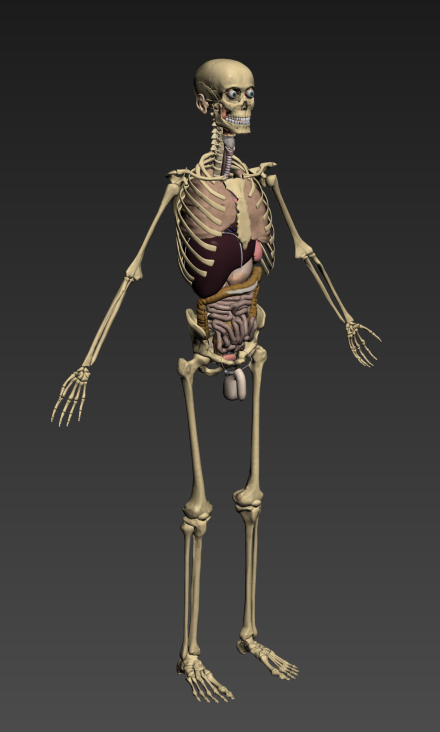
\includegraphics[width=0.32\linewidth]{figures/3-IMR/muscleSkeleton}}
%%	\caption{Anatomy model from ANATOMIUM 3D}
%	\label{fig:3-IMR:humanModel}
%\end{figure}
Since the application covers just one arm and quite a few simple motions, this muscle and skeleton model was simplified under the supervision of a senior medical student. Only the bones of the arm and the shoulder, and the muscles responsible for the motions, flexion, extension, pronation, and supination, are chosen, i.e. the \textit{musculus biceps brachii, musculus triceps brachii, musculus brachialis, musculus anconeus, musculus pronator teres, musculus pronator quadratus and musculus supinator}. The \textit{musculus coracobrachialis} is added to this collection according to the medical partner's suggestion, although it does not contribute to the motions mentioned above.

The bone models are used as they were, but after consulting with medical professionals, we decided to recreate the muscle models, since the existing ones did not resemble their real counterparts closely enough. 
%The biceps and triceps are presented as two and three separate parts, respectively, and the position of the anchor points of most muscles do not correspond to their real-world position. 
To achieve a more realistic visual effect, the muscle model should be deformed during the selected motions.
The texture of the 3D muscle model is realistic, especially in a close up view. But it is quite difficult to apply vertex weights to the mesh topology of the original muscle model. 
In this application , most muscles are modeled with a cylindrical base mesh and created using polygonal modeling techniques and subdivision algorithms according to images from the Sobotta Atlas of Human Anatomy (see \figurename{\ref{fig:3-IMR:modifiedArmModel}}). Only the \textit{supinator} and the \textit{pronator quadratus} are modeled from a flat box, due to their shape. The biceps and triceps are both created as one contiguous model instead of separate parts for each head and detailed attention is given to the anchor points for all muscles to make sure they are at the correct positions.
\begin{figure}[htb]
	\centering
	\subfloat[Flexors]{\label{fig:3-IMR:modifiedArmModel:a}
		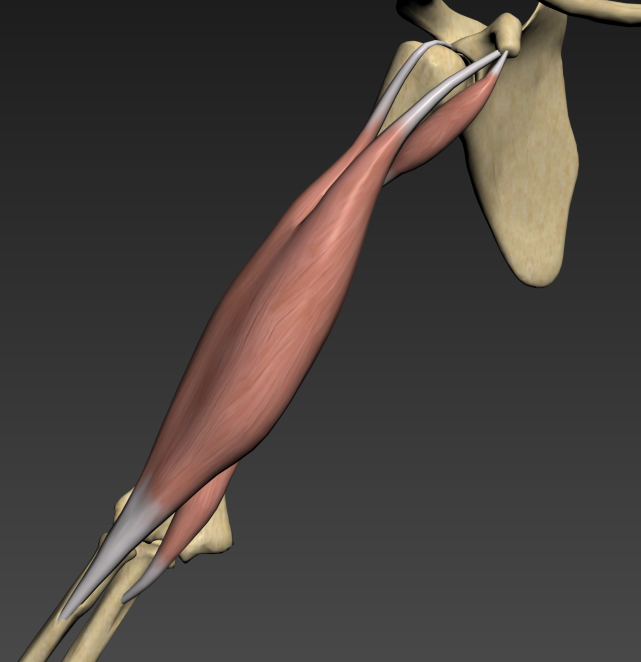
\includegraphics[width=0.32\linewidth]{figures/3-IMR/muscleFlexor1}
		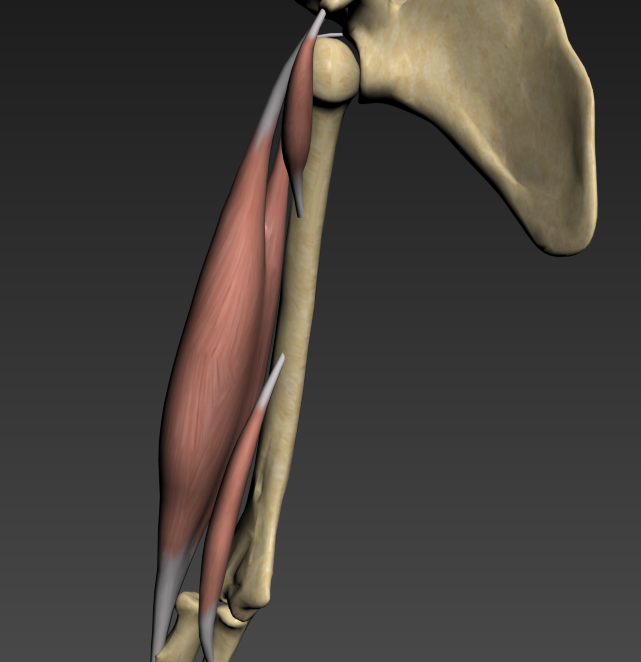
\includegraphics[width=0.32\linewidth]{figures/3-IMR/muscleFlexor2}
		}
	\quad
	\subfloat[Extersors]{\label{fig:3-IMR:modifiedArmModel:b}
		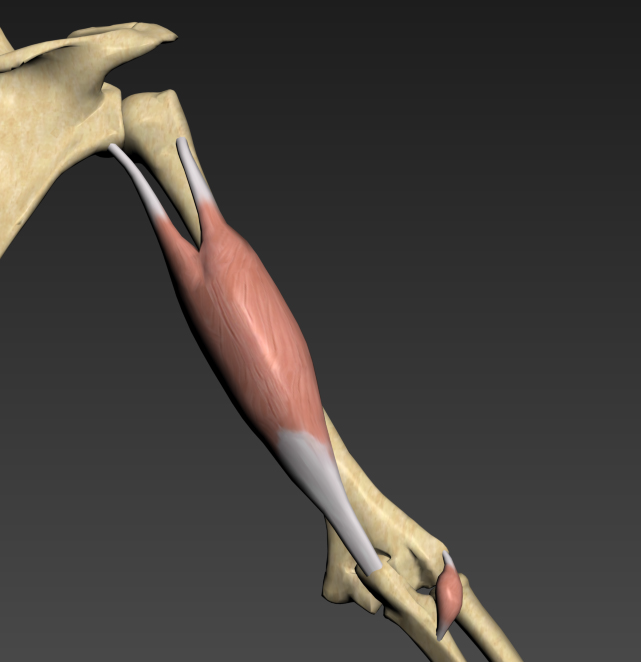
\includegraphics[width=0.32\linewidth]{figures/3-IMR/muscleExternsor}}
	\subfloat[Pronators]{\label{fig:3-IMR:modifiedArmModel:c}
		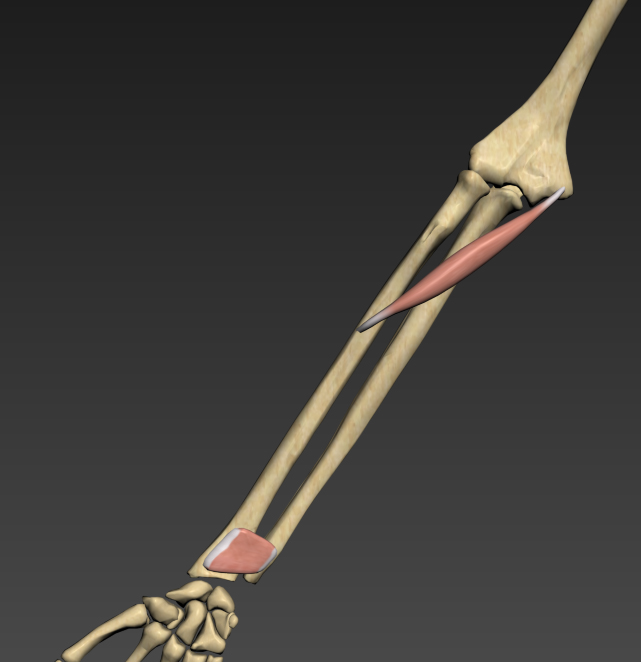
\includegraphics[width=0.32\linewidth]{figures/3-IMR/musclePronators}}
	\subfloat[Supinator]{\label{fig:3-IMR:modifiedArmModel:d}
		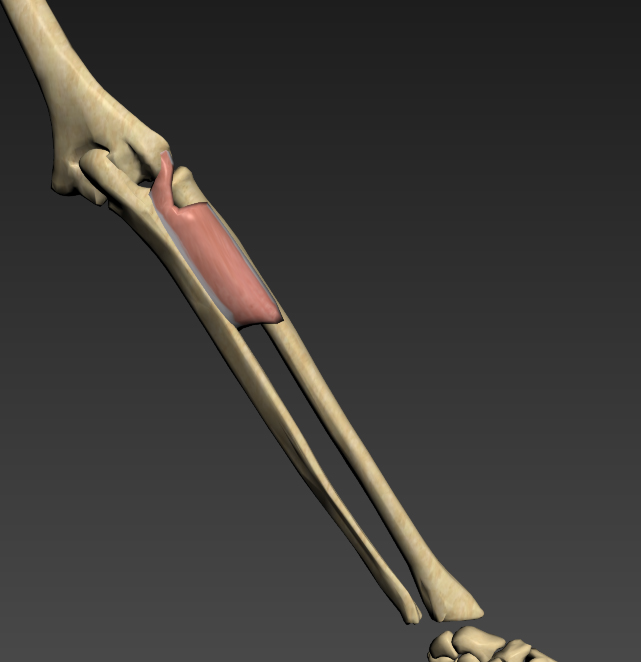
\includegraphics[width=0.32\linewidth]{figures/3-IMR/muscleSupinator}}
	\caption{Dynamic Muscle Models. Most muscles were modeled with a cylindrical base mesh that was modified using polygonal modeling techniques and subdivision algorithms according to images from the Sobotta Atlas of Human Anatomy. Each picture shows the muscles involved in each motion.}
	\label{fig:3-IMR:modifiedArmModel}
\end{figure}

\paragraph{Muscle deformation} To enable the animation of the arm model, the bones are weighted to different armatures that consists of one control object. 
The ulna and radius are weighted to separate control objects to behave correctly when the hand is rotated. 
To deform the muscles, the vertices of each model are weighted to several control objects, which can be transformed easily according to the bones (see \figurename{\ref{fig:3-IMR:modelArmature}}). 
The vertices follow the transformation of each related object to a special percentage, which is determined by their weighting. 
\begin{figure}[htb]
	\centering
	\subfloat[Arm Model]{\label{fig:3-IMR:modelArmature:a}
		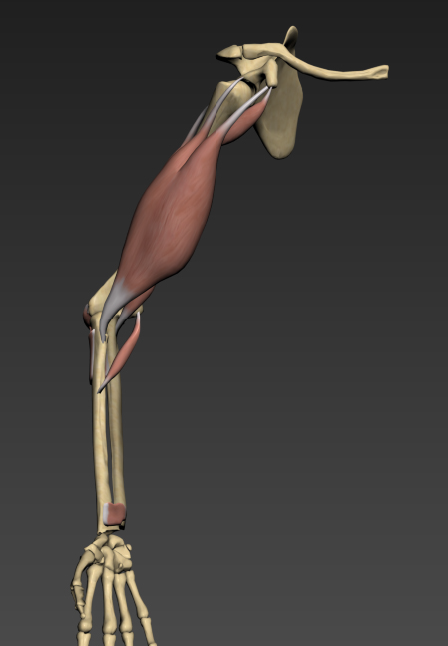
\includegraphics[width=0.32\linewidth]{figures/3-IMR/ArmatureMuscle}}
	\subfloat[Armature]{\label{fig:3-IMR:modelArmature:b}
		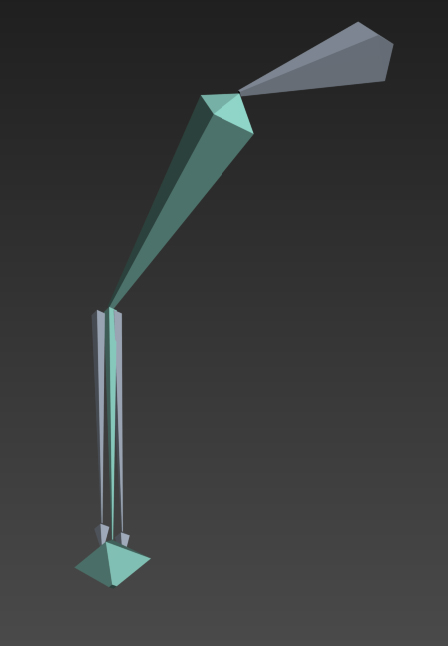
\includegraphics[width=0.32\linewidth]{figures/3-IMR/Armature}}
	\subfloat[Armature with Muscles]{\label{fig:3-IMR:modelArmature:c}
		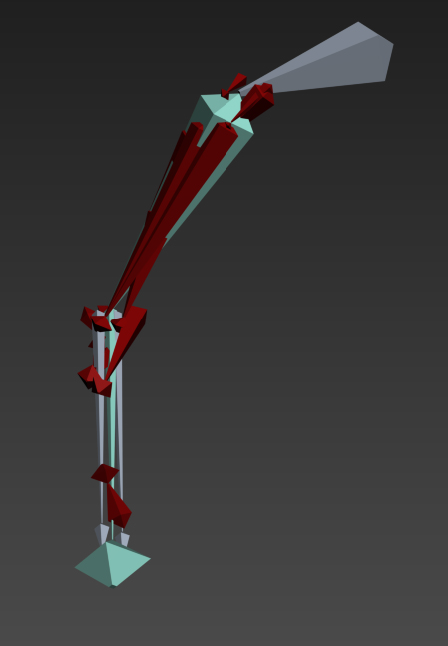
\includegraphics[width=0.32\linewidth]{figures/3-IMR/ArmatureWithMuscle}}
	\caption{Dynamic Muscle Models. The bones are weighted to different armatures and the vertices of each model are weighted to several control objects in the armetures.}
	\label{fig:3-IMR:modelArmature}
\end{figure}
The muscles' animation for contraction and expansion was achieved in 3DS MAX\footnote{\url{http://www.autodesk.com/products/3ds-max/overview}} via stretchy bones, which automatically contract or expand, if their length is changed. 
Whenever a new user is detected, the neutral length of each muscle is recalculated after the skeleton is scaled.
This is accomplished by a configuring class attached to each muscle's control object. It contains references to the control object's two anchor points and uses them to define its position and rotation. The position is set directly to that of the first anchor point, while the rotation is calculated via a relative rotation.
The application measures the distance between the control object's anchor points and scales it along its local x-axis according to the ratio between that distance and its neutral length. Along the y- and z-axis the inverse of that ratio is used for scaling, multiplied by a factor to control the magnitude of expansion. 

\subsubsection{Learning functions}
\paragraph{Virtual view}
The details of the muscle are very important, so a virtual view is introduced to present a close up view of the arm model to show the attachment points and the spatial relationship. There are several solutions to place the virtual camera. One is that the camera rotates around a special object and generates the virtual view from different angles. The cameras are attached to a rotating helper object to create an orbiting movement around the arms. 
%Additionally, it can be influenced by the user in order to have an even closer look at areas of interest. In all views, the active muscles are highlighted.
The close views are implemented with additional cameras and copies of the arm model. By putting these copies into separate layers it is ensured that these cameras only render their respective objects. The first copy takes part in just the flexion and extension, while the second one participates in the pronation and supination. The muscles, which are not responsible for the selected movement, are removed, to keep them from obscuring the relevant muscles or occlude them.
\begin{figure}
	\centering
	\subfloat[View 1]{ \label{fig:3-IMR:MuscleLearningVirtualCamera:a}
		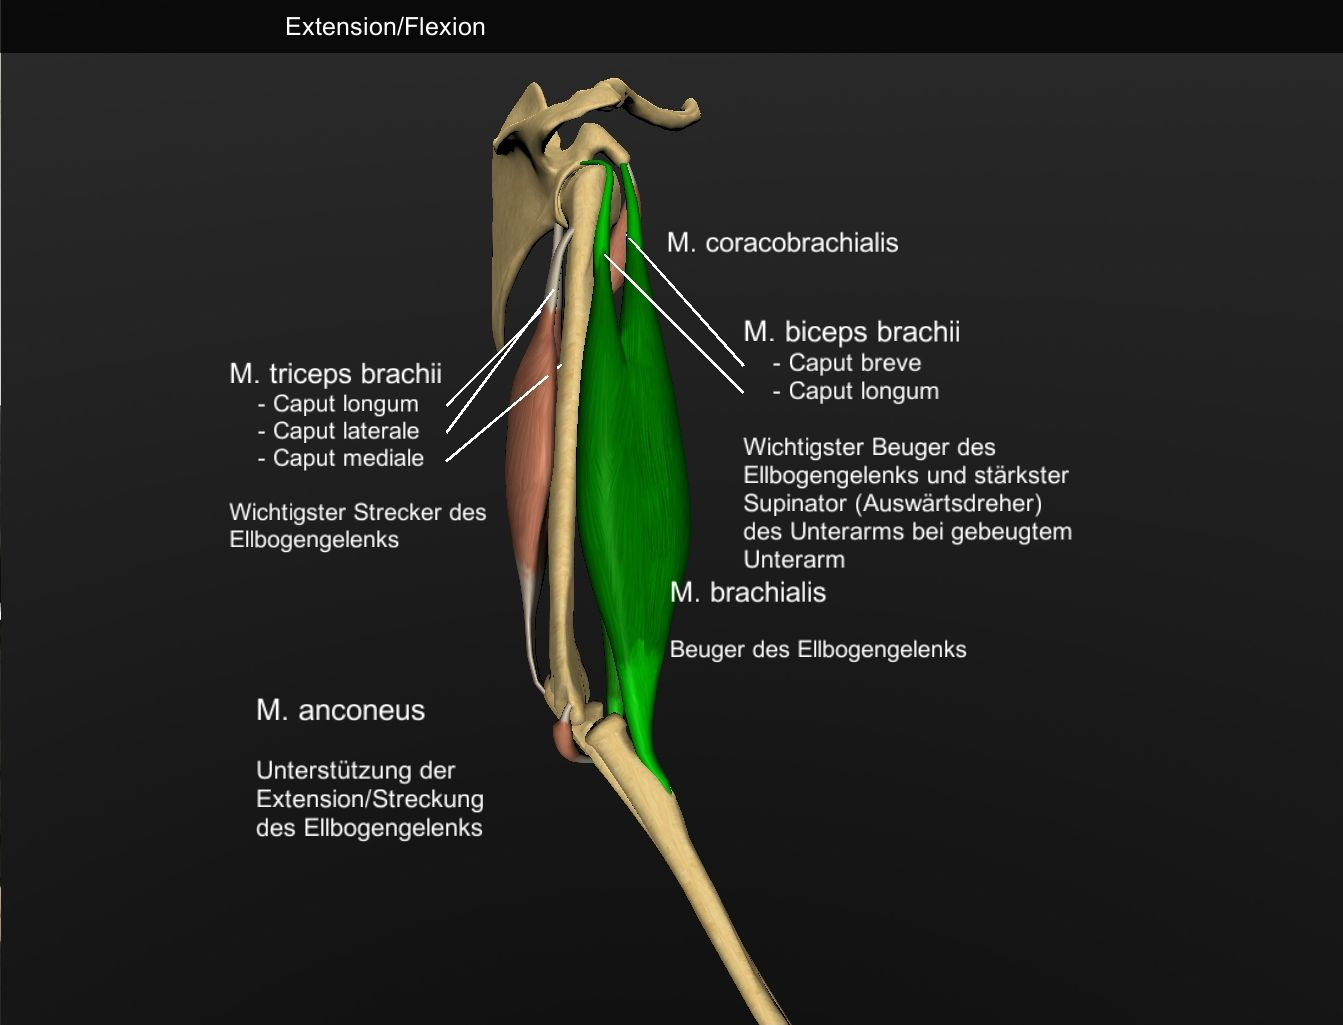
\includegraphics[height=0.4\linewidth]{figures/3-IMR/MuscleLearningVirtualCamera}}
	\subfloat[View 2]{ \label{fig:3-IMR:MuscleLearningVirtualCamera:b}
		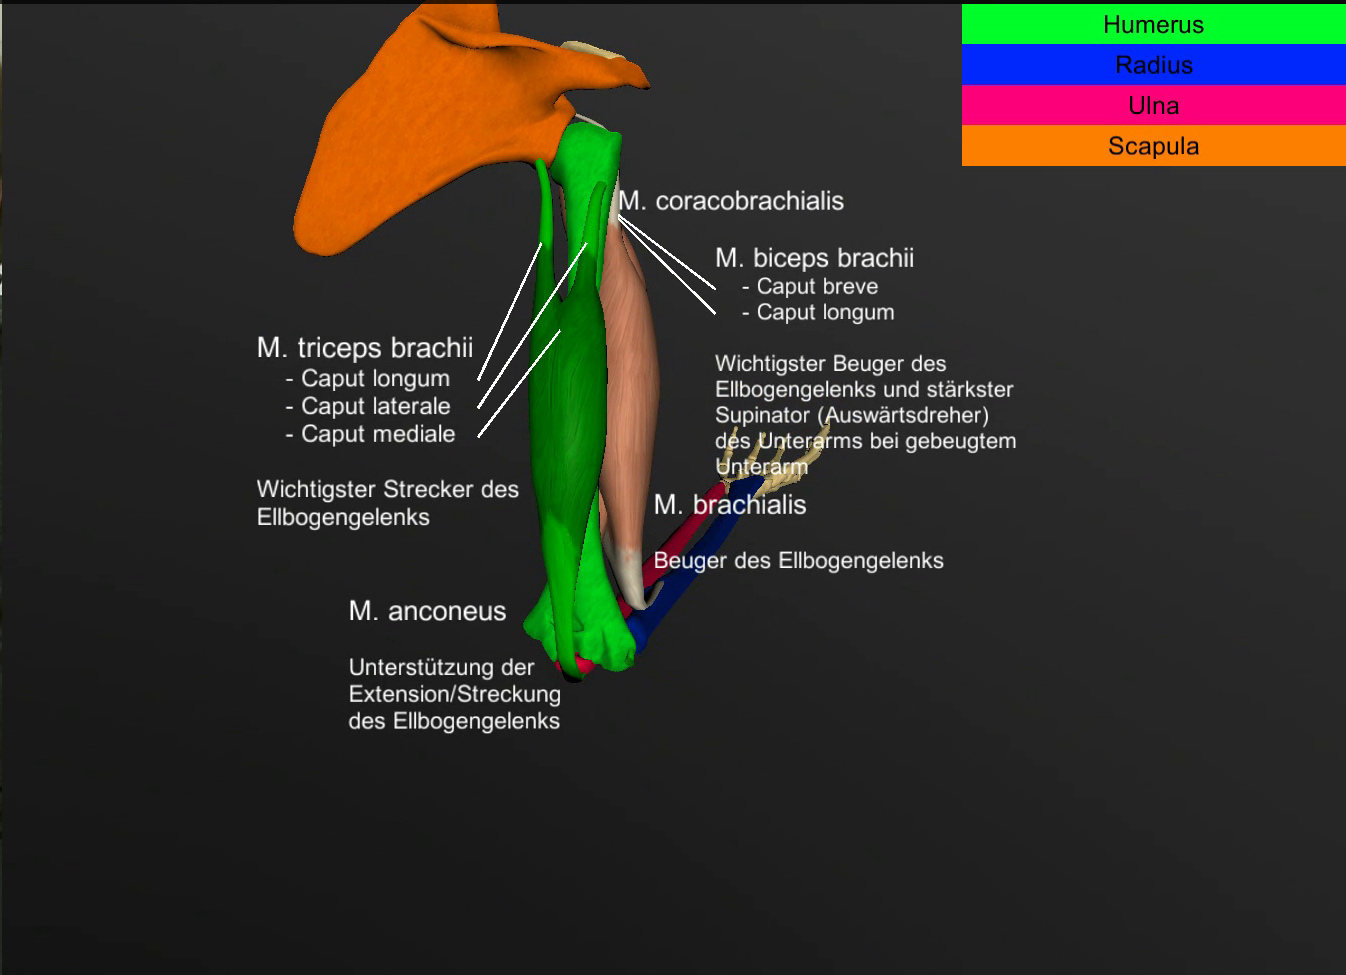
\includegraphics[height=0.4\linewidth]{figures/3-IMR/MuscleVirtualCamera}}
	
	\caption{Virtual Camera concentrating on Flexion and Extension.}
	\label{fig:3-IMR:MuscleLearningVirtualCamera}
\end{figure}

\paragraph{Self-control virtual view}
A self-control virtual camera is introduced and its position and rotation can be controlled by the user. When the user's right hand is placed close to the left arm, the self-control camera model is triggered. The camera moves to the position of the hand and tries to focus on the desired area by calculating the closest point on the arm and rotating towards it (see \figurename{\ref{fig:3-IMR:selfControlCamera}}). This point is computed in the user-controlled arm's local coordinate system and transformed into that of the arm currently observed. As shown in \figurename{\ref{fig:3-IMR:MuscleLearningSelfControlCamera}}, the user can naturally move the virtual camera to focus on different objects from different view angles. This function introduces more friendly interaction for muscle learning.
\begin{figure}
\centering
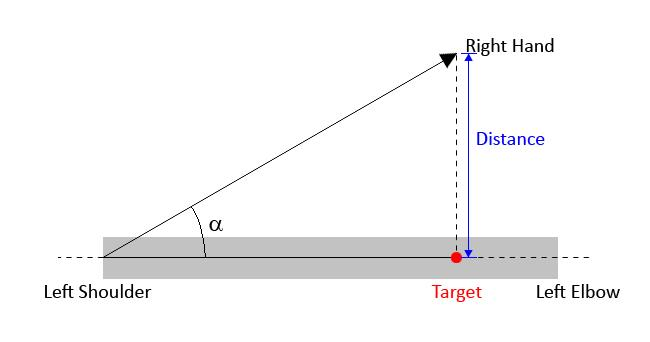
\includegraphics[width=0.7\linewidth]{figures/3-IMR/selfControlCamera}
\caption{The camera moves to the position of the hand and tries to focus on the desired area by calculating the closest point on the arm and rotating towards it.}
\label{fig:3-IMR:selfControlCamera}
\end{figure}

\begin{figure}
	\centering
	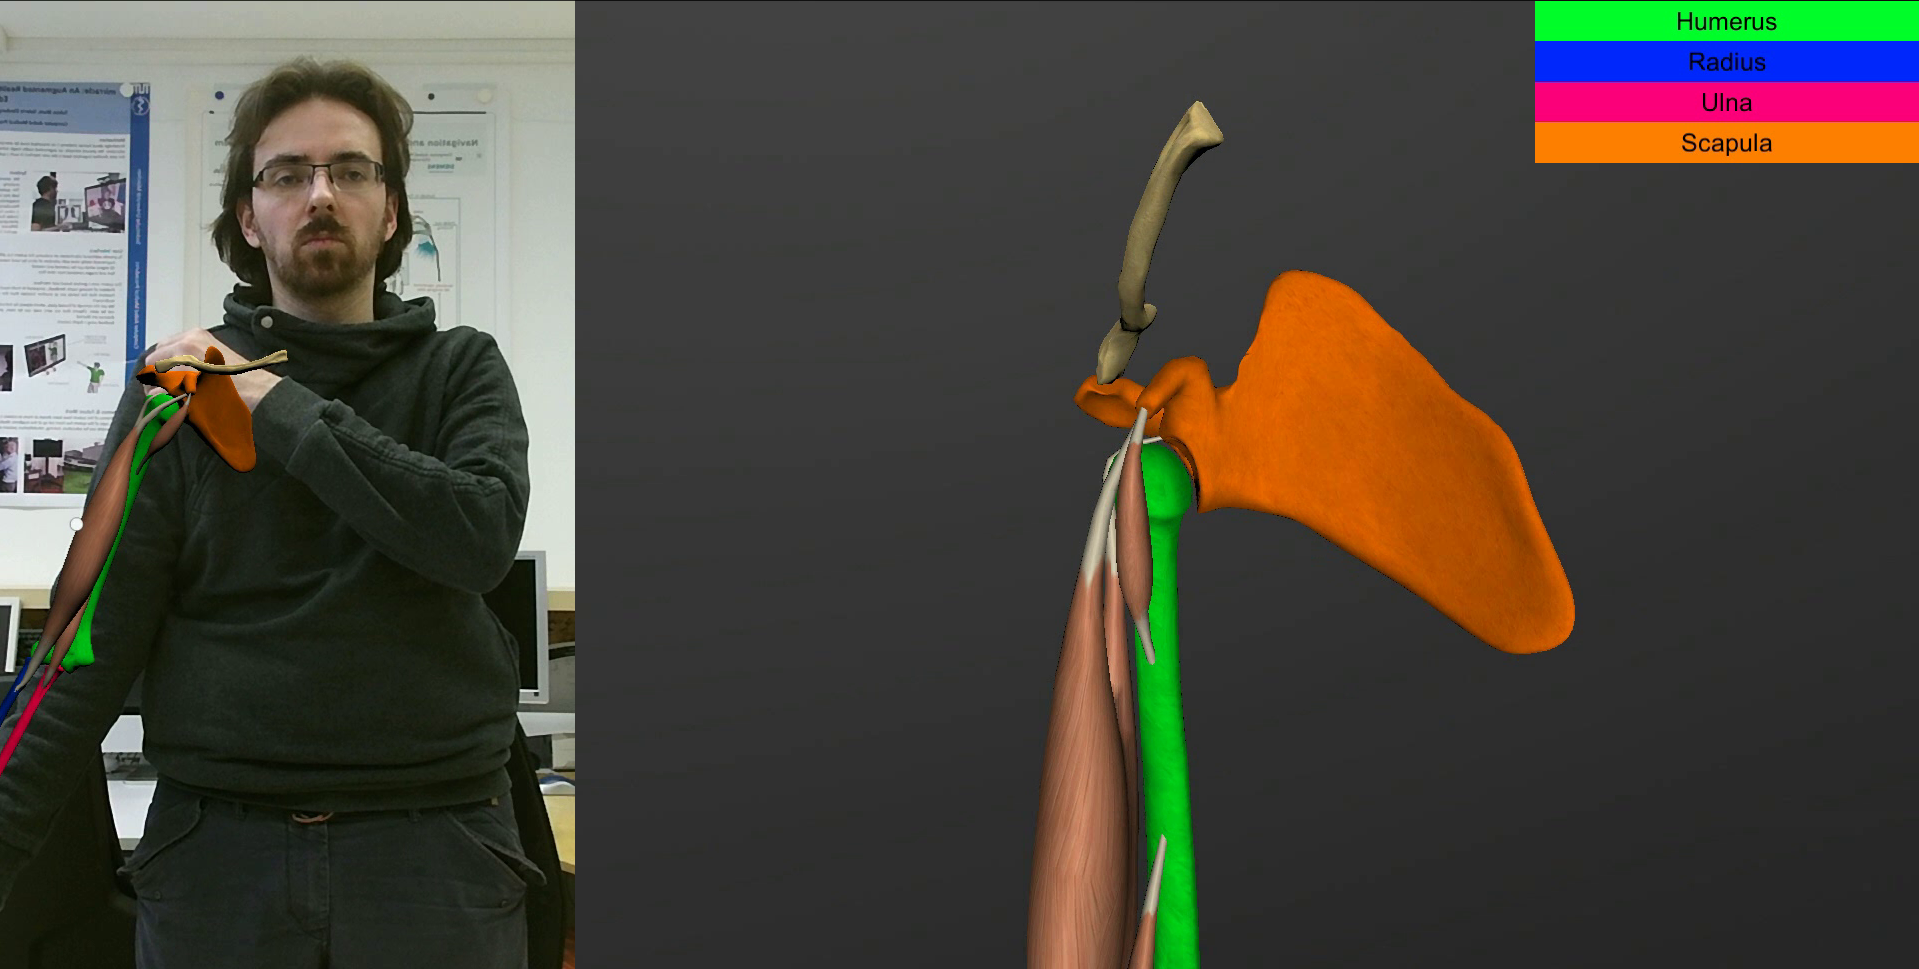
\includegraphics[width=0.8\linewidth]{figures/3-IMR/MuscleLearningSelfControlCamera}
	\caption{When the user's right hand is placed close to the left arm, the self-control camera model is triggered.}
	\label{fig:3-IMR:MuscleLearningSelfControlCamera}
\end{figure}
\paragraph{Interactive learning}
A configuring class is defined, including methods to control the muscles' visibility, the highlighting of working muscles and of anchor points, and the labels that display the muscles' names and function. For highlighting it determines the angle between the upper and lower arm, as well as the rotation of the hand, relative to the frame before. This information is used to determine which motion is being performed, and in turn which muscles are active according to \tablename{\ref{tb:3-IMR:motionMuscles}}. 
%In an earlier prototype, each muscle controlled the highlighting itself by measuring the change in length, but this data proved to be too inaccurate and produced noticeable flickering. 
%The abstraction using only the angles between the joints of the arm yielded smoother results. 
Additional functions are created to toggle the visibility of all muscle-labels to the user interface and control the visibility of muscles by type.
Similar to the muscles, the bones are controlled by a configuring class. These determine the color-coding of the bones and expose this functionality to the UI.
In the muscle oriented model, one or more muscles are shown successively and the AR view and virtual view of the muscle is generated. The user can perceive the detail of the muscle, the start and end point and the spatial relationship with the bone (see \figurename{\ref{fig:3-IMR:muscleModelLearning}}). 
In the motion oriented model, users are asked to perform special arm movements and only the muscle involved is highlighted (see \figurename{\ref{fig:3-IMR:MuscleLearningVirtualCamera:b}}). Then the functions of the muscle are learned. 
During the learning procedure, the user can always move the arm and see the muscle state and shape deformation.
When a motion is performed, active muscles would be visually highlighted in order to make them more prominent.
\begin{figure}
\centering
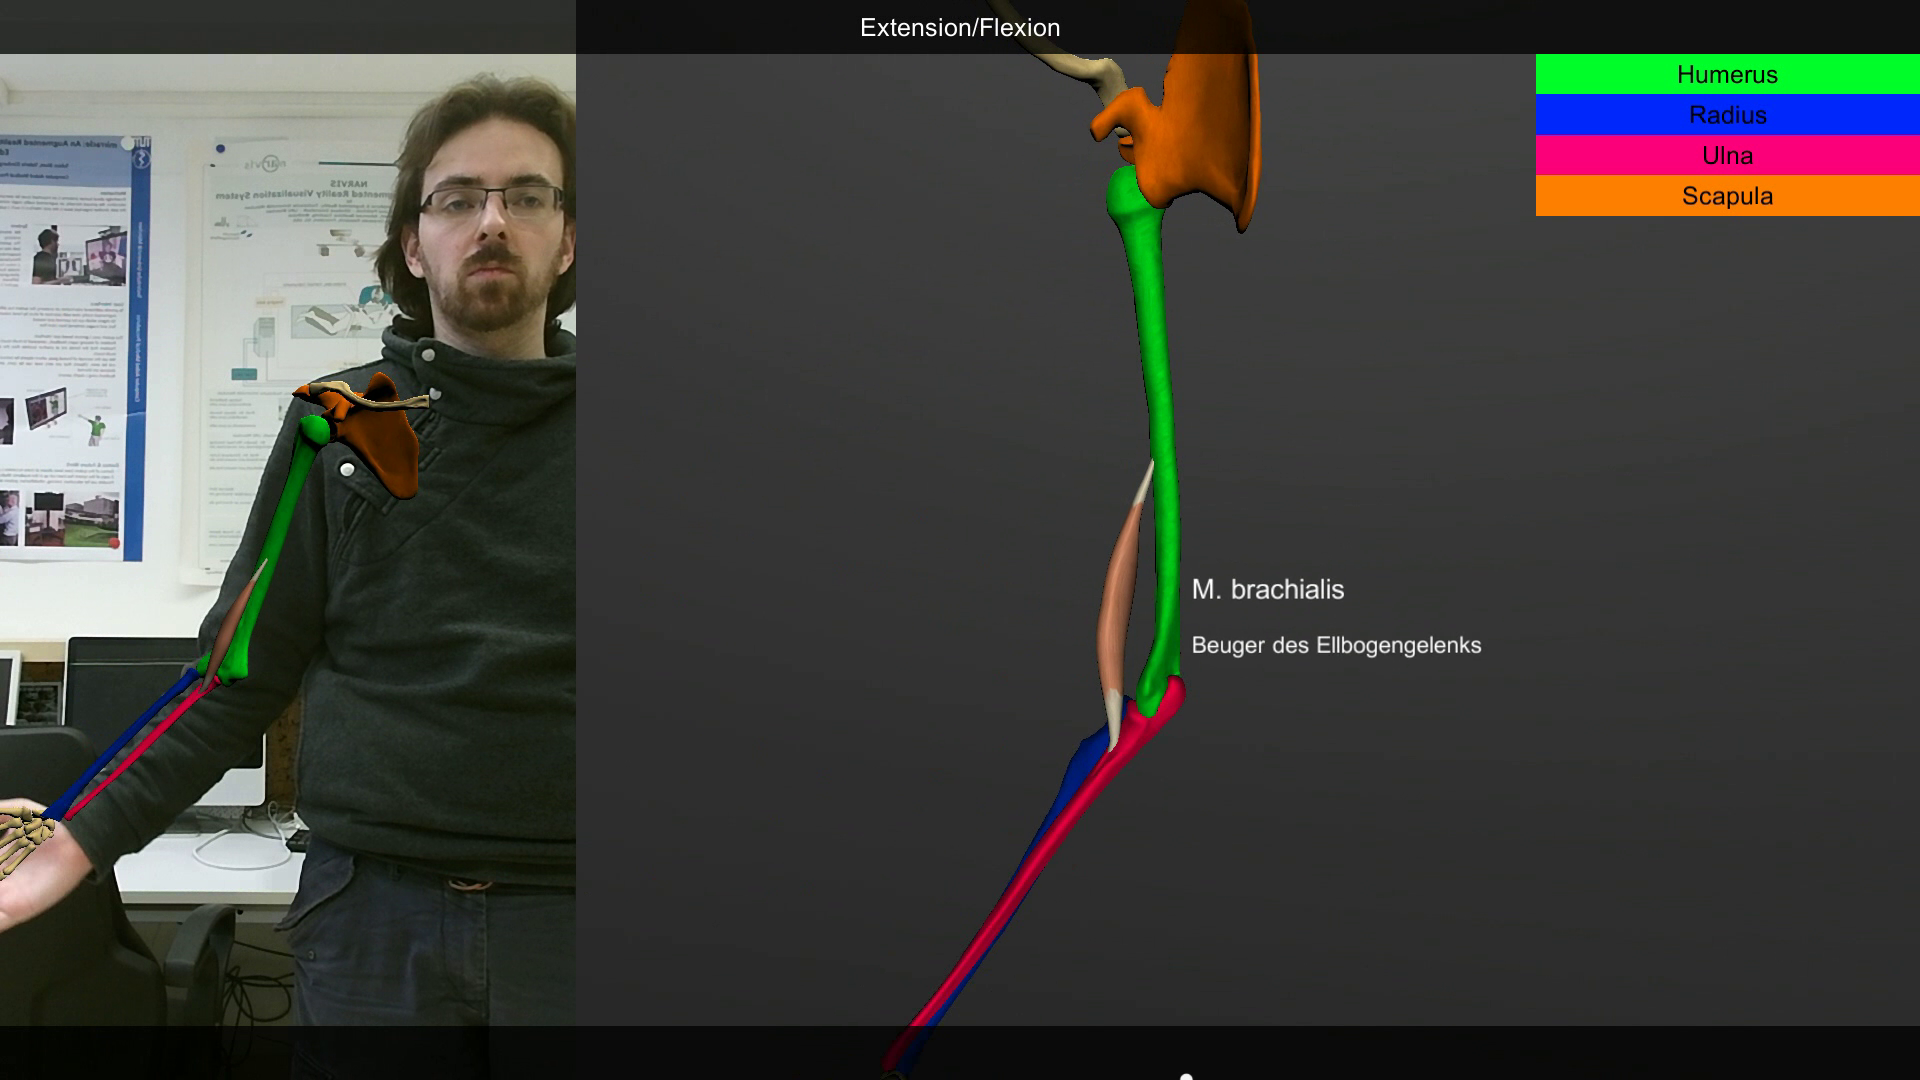
\includegraphics[width=0.8\linewidth]{figures/3-IMR/muscleModel}
\caption{Muscle oriented model: one muscle is shown and the user can perceive the detail of the muscle, the start and end points, and the spatial relationship with the bone.}
\label{fig:3-IMR:muscleModelLearning}
\end{figure}

\paragraph{Learning Sequence}
Based on the AR and Virtual view, the system can generate a lot of learning material. We prefer a simple user interface and let the user focus on the learning instead of how to control this system. 
%However, natural interaction would not introduce any barrier. 
Hence, we introduce another function, ``Learning Sequence''.
The sequence of events for the learning session is predefined via a configuring file. This is an easily editable text format with values separated by semicolons. Each line in this file contains the data for one event. The data for one event consists of an integer for the duration and the camera mode, boolean values to enable or disable the color-coding for the bones, the muscles' labels and highlighting of their anchor points, and a bitmask that determines the muscles visibility. Each bit in this eight-digit binary number controls visibility for one muscle. An optional seventh value can be used to display text at the bottom of the screen. 
This file is opened and read line after line by a simple parser at the start of the program, and the data is stored in an array of event structures. 
The sequence is played using a coroutine that takes one entry from the event-array and uses its values to set the relevant parameters and waits for the specified time before triggering the next event, until it reaches the end of the array. Simple functions can control the running sequence by stopping and restarting the coroutine or by modifying the array-index to skip or replay events.

To facilitate the learning session, the users run through a predefined sequence of events. The learning sequence can be generated according to the user's needs. Here is one example. 
It starts with the AR-view, showing the bones of the arm, identified by color, with the muscles hidden. It then switches to the first close view to introduce the muscles for flexion and extension individually. Next to each muscle is a label displaying its name and additional information about its function. After the muscles contributing to each motion have been introduced, they are shown together to give the user the opportunity to recap. This process is then repeated for pronation and supination. 
The whole sequence runs for approximately ten minutes and can be stopped, paused or resumed at any time. Additionally, it is possible to skip events or return to passed ones. Both the color-coding and the labels showing the muscle-information can also be displayed independently from the learning sequence.

%\subsubsection{Evaluation}
%todo data from Ina's thesis
%\subsubsection{Discussion}
Based on our discussion with medical students we found that they really liked the AR visualization on their own bodies, however they were not used to the natural user interface and gestures required for interaction. A learning curve was necessary for them to appease initial frustrations they had when first using our system.
%The users were divided into two groups, the first of which used the application, while users from the second group were handed conventional materials, i.e. a section from an atlas of human anatomy, to learn the same information. Both groups got twenty minutes to acquire as much information about the arm as possible, which meant for those using the application to run through the sequence twice. 
%After this time was up, each user was to fill out a questionnaire.
%By the time of writing the results of the study was not yet analyzed, but from the witnessed sessions it became apparent that 
Most students who tried the application viewed it as an interesting and engaging source of information. The possibility of viewing the arm from every direction offered them a new insight that they could not get from static images. The students confirm the effectiveness of acquiring knowledge with an AR-program. However, this application is limited by necessity, so the textbook still constitutes a more universal resource and it can function as a useful supplement. 
%If the study confirms the effectiveness of acquiring knowledge with an AR-program, a further developed application could possibly include and convey a higher percentage of the information offered in the book, but the feasibility of replacing it completely seems debatable.

%\subsection{musculoskeletal Animation} \label{sec:3-IMR:musculoskeletal}
%Instead of rendering the bones from a rigid CT dataset, a polygonal model will be used to create the AR view of the skeleton. Then, we can animate the model based on the orientation of the joints received from the skeleton stream to match the pose of the user in front of the system.
%The objective of this application is to develop a simple non-physical visual effect of the musculoskeletal system based on models from OpenSim\footnote{\url{https://simtk.org/home/opensim}}, which is freely available, user extensible software system that lets users develop models of musculoskeletal structures and create dynamic simulations of movement. Besides mirroring the users movements to the skeleton, the system also visualizes the relationship between bones and muscles. Furthermore, a labeling system is implemented which can be used to teach the user names of the muscles or bones (see \figurename{\ref{fig:3-IMR:skeletonMuscleDemo}}).
%
%\begin{figure}
%	\centering
%	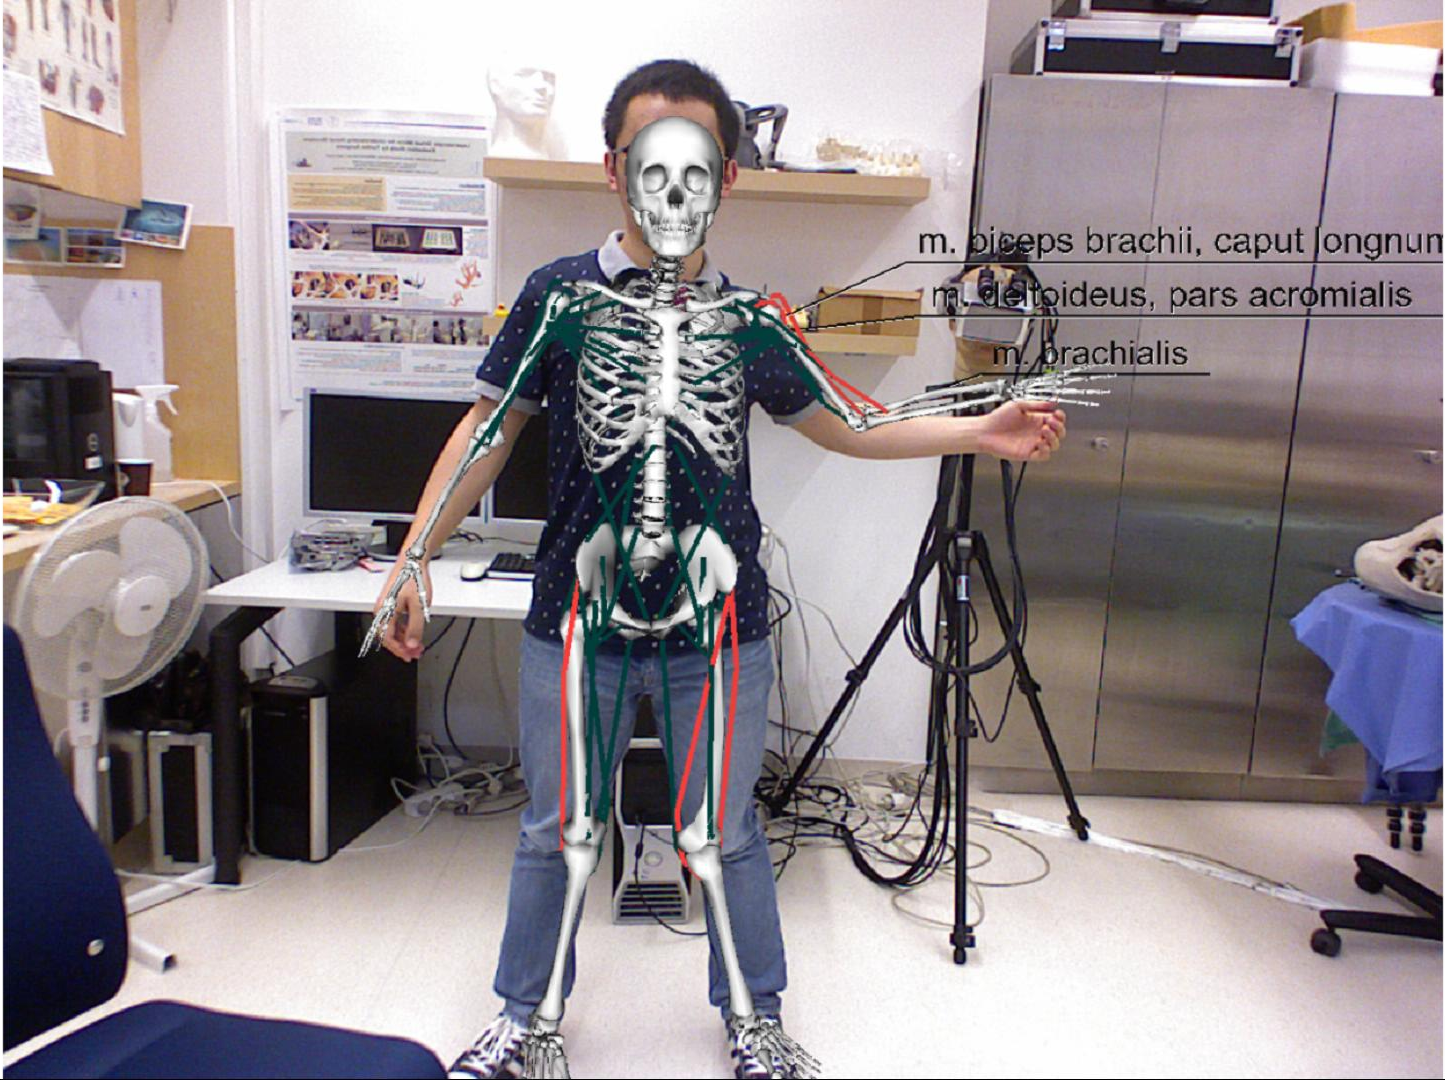
\includegraphics[width=0.7\linewidth]{figures/3-IMR/skeleton_Muscle2.png}
%	\caption{Musculoskeletal Animation in Magic Mirror: an application to show a simple non-physical visual effect of the musculoskeletal system based on models from OpenSim}
%	\label{fig:3-IMR:skeletonMuscleDemo}
%\end{figure}
%
%\subsubsection{OpenSim Musculoskeletal Model}
%OpenSim is an open source software platform for biomechanical modeling, simulation, and analysis. The GUI includes many tools for loading data, creating and editing models, visualization of the simulation results, and much more. The API allows programmers to access the core components of OpenSim to create new plug-ins for the GUI or take advantage from it in theirs own applications. It also includes some validated musculoskeletal models and more can be downloaded from the platform website\footnote{\url{www.simtk.org}} where researchers can provide their work \cite{Delp2007}.
%
%OpenSim Musculoskeletal Models consist of bodies, joints, forces, constraints, controllers, markers, and contact geometry (see \figurename{\ref{fig:3-IMR:openSimModel}}). The skeleton is build up with rigid bodies and joints connecting two bodies. A body has attributes for its mass, center of mass, and inertia. It can include display geometry for bones. Joints have an attribute for their position in the parent body and hold a joint type dependent transformation to define the motion of a body relative to its parent body. Movements can be further restricted by constraints. Muscles are modeled as forces that are exerted on attachment points to the rigid bodies. The force of the muscle is dependent on its path (through all the attachment points) and muscle properties like maximum force, optimal fiber length, tendon slack length, pennation angle, and maximum contraction velocity. 
%From the OpenSim models, we can definitely use the skeleton model and the paths of the muscles, by a conversion of the geometry data and reorganization of the scene graph. But, the muscle states simulation functions are difficult to integrate into Magic Mirror system, since it can not calculate the muscle activity in real time.
%\begin{figure}
%	\centering
%	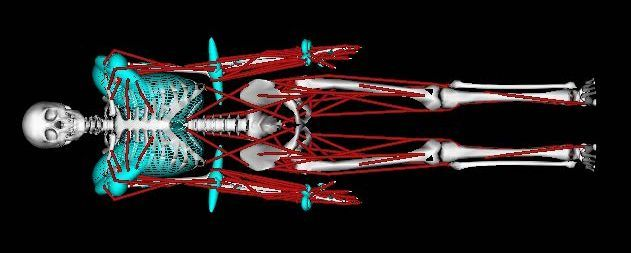
\includegraphics[width=0.8\linewidth]{figures/3-IMR/openSimModel.png}
%	\caption{OpenSim Musculoskeletal Model: The skeleton is build up with rigid bodies and joints connecting two bodies. Muscles are modeled as forces that are exerted on attachment points to the rigid bodies. }
%	\label{fig:3-IMR:openSimModel}
%\end{figure}
%
%\subsubsection{Application Design}
%Based on the Magic Mirror framework, the application is designed according to the following rules. The objective is a simple interactive MR application for education.
%\begin{itemize}
%	\item Accurate AR view of the skeleton.
%	\item Clear relationship between the bones and muscles.
%	\item Estimate the muscle active states when the user performs movements.
%	\item Highlight the active muscle according to the movements.
%	\item Information of the bones and muscles for learning.
%\end{itemize}
%A general musculoskeletal model is created according to the OpenSim models and it contains the bone geometry, connections between the bones, muscles and attachment points to the bones. Skeleton and muscles are load to the application as two separated sub scene graphs, as  the skeleton model can be used independently for many purposes. In real world, the muscles control the bone movements, but the muscle model is dependent of the skeleton model in the application as the system input are just the positions and orientations of the skeleton joints. The skeleton model is transformed based on the skeleton stream from the Kinect and the muscle model is then updated as it is affixed on the bones via the attachment points. Both models are rendered to create the non-physical visual effect to generate the AR view. 
%
%\paragraph{Update Skeleton Model}
%After a user is calibrated, the skeleton model is scaled to fit the current body. The proportion of the user can be estimated through the pose matrices. The scale method first scales the root node which is the pelvis and it actually scales the whole model. 
%The scale factor is calculated from the distance of the right shoulder to the left hip. So this scale factors represents the average of width and height of the torso relative to the general model. In practice using this approximation gave better results then calculating two different scale factors. 
%The accuracy of the proportions of the legs could be improved by calculating the distances between hip, knee, and ankle. We employ the same scale as the torso when the knees and ankles are not observed by the sensor.
%Here we also define a calibration pose to get an accurate measurement of the segment length. 
%The calculation of the transformation of each joint on the model is also another important task. The relationship between the coordinates spaces of Kinect, OpenGL, and the skeleton model has to be carefully analyzed. In order to obtain the correct relative rotation of each bone, quite a few transformations have to be apply to the raw joint orientation from skeleton stream. The skeleton model is then animated to mirror the body movements.
%
%\paragraph{Update Muscle model}
%The muscle model contains all the individual muscles, which is displayed in the application. Each muscle is model as a 3D string which goes through all the attachment points. So the muscle model is dependent of the skeleton model and is first created based on the general skeleton model. Wherever the skeleton model is updated, each muscle model is also recreated to make sure the size and special relationship is correct. 
%
%%add an attachment point to define the path of each muscle model 
%The attachment point information for each muscle is textually found inside the OpenSim 'osim' model file. Each attachment point is defined by the bone's name, 3D position in the bone coordinate system, and the type of point. One muscle has several attachment points, which define the relationship with the bones. A xml file is create to save all muscle information.
%In the application, 3D strings are rendered between each pair adjacent attachment points. 
%The color of the string is defined as the active state of the muscle and the line width can be adjust according to the muscle's size. The muscle model is not hierarchical as the skeleton model. Muscles are attached to bones in different coordinate systems. As the attachment point is defined in the bone coordinate system, the positions have to be converted to the world space. The world position of the bone is easily calculated by accumulating all the transformations from the skeleton root to the current bone object. Then, each attachment point can be converted to the world space.
%
%A Label class is designed to show text information of the bones and muscles. The Label is meant to display text attached by an arrow to a point in the scene. The special feature of this class is that two labels will never overlap. The originating point of each label is from the object, e.g., a bone or a muscle, and where the text is actually drawn depends on the sorted vector of the all visible labels. The text is drawn always below the text of the label previous and connected with a line to the originating point (see \figurename{\ref{fig:3-IMR:openSimModel}}).
%
%%update muscle color 
%When a new frame comes in, the system updates the skeleton model according to the orientation of the each joint. And the world coordinates of each bone and attachment points are calculated. The length of each muscle can be estimated by the distances between the points. The active state of the muscle can be simple assessed based on the length change. A muscle is active when its lengths is shorter than the initial length or at least shorter than its previous length.  In this case the color will be scaled between red and green dependent on the difference. Red means that the muscle is active and green means that the muscle is approximately inactive. It depends on the contraction speed and the length of the muscle. This method does not compute forces like OpenSim, it only estimates the activeness of the muscle very coarsely. Finally, muscles are redrawn with the new position and new color.
%
%OpenSim provides some advanced function to simulate the active states of the each muscle based on the body movement, but the approximation in real time is not possible right now and only the skeleton position stream is too noisy for such simulation. Another possible solution to fetch more accurate muscle state is to attach electromyographic sensors onto the user's body. This should be one of the future work for this thesis. 
%%In the next step the color of the muscle is recalculated.
%%The color is going have a portion of green of intensity and a portion of blue of 1-intensity. The intensity is defined as the square difference of the length and previous length of the muscle normalize by the initial length. So the intensity is influenced by the speed of the contraction. If the length of the muscle is shorter than the initial length then one can average it with intensity2 for the actual amount of contraction to simulate gravity.The formula for intensity  is obtained experimentally.
%%If the muscle is active this is calculation of the color:
%%\begin{figure}
%%\centering
%%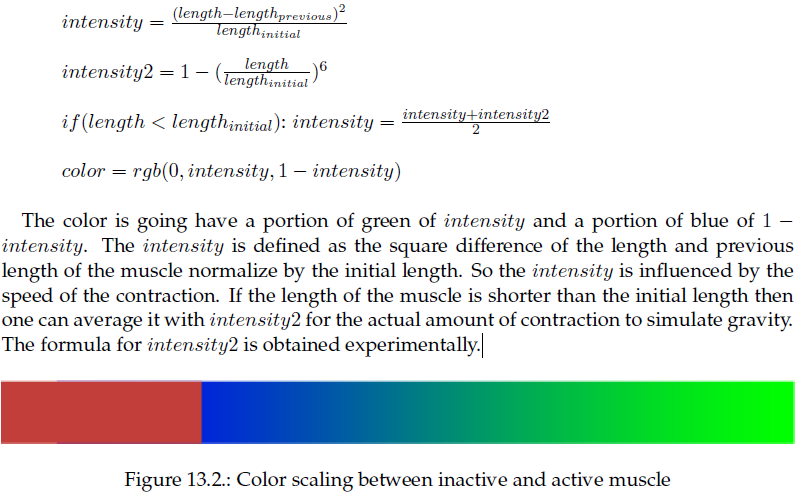
\includegraphics[width=0.7\linewidth]{figures/3-IMR/mulcleActiveColor}
%%\caption{To calculate the muscle active state and the color mapping function}
%%\label{fig:3-IMP:mulcleActiveColor}
%%\end{figure}

\subsection{Serious gaming for rehabilitation} \label{sec:3-IMR:gaming}
Leg injuries are common injuries in both sports and everyday life. After some complicated injuries many patients can not use their leg for a long period. Following this lengthy healing progress, a period of rehabilitation is required to restore functionality and resilience of the injured leg. Various rehabilitation exercises are used by physiotherapists to increase the patient's ability to keep balance. 
These exercises include balancing on one leg and moving the other leg or arms, or even simple weight shifting exercises. Other exercises require the patient to stand on one leg, bend their knee slightly and balance with a straight back. Balance boards can also be used to increase the difficulty of the balancing exercises. These rehabilitation exercises are tailored towards every patient individually and are often supervised by a physiotherapist. The conventional exercises are typically repeated many times which makes them tedious and feel like a chore.

Motor rehabilitation consists in iterative repeating exercises to strengthen the affected body area. Since the rehabilitation must be performed over quite a long period it is common for patients to get disinterested, and consequently, they perform the exercises in a casual and incorrect manner. 
Usually, motor rehabilitation occurs by regular meetings between patient and physiotherapist with  depending on the availability of both. We believe that it becomes crucial for the patient to perform exercises at home to speed up the rehabilitation process. However, at home both therapeutic instructions and corrections by the therapist are not verbally provided to the patient, which potentially leads the patient to perform the exercises incorrectly.
%Health education and rehabilitation is a particular area where serious gaming is suited \cite{Aubin2012,Jonas2012}.

A serious game for balance rehabilitation is developed for leg stability and balance training. It is designed to entertain the user while doing the exercise as well as monitor and correct the patient. To deliver motivation, the exercise has to entertain the patient via the Magic Mirror effect. It will encourage the user to continue the exercise and accelerate the healing process. The game also takes over monitoring work from physiotherapists, so the patient can do exercises on their own. It offers self-monitoring of stances, such as ``standing on one leg'' or ``standing straight'' and displays messages to warn the patient if they fail to keep their balance or stance.
The resulting game is tested by patients and reviewed by doctors and physiotherapists to assess its usefulness with regard to motivating the patient and its usefulness from the medical perspective \cite{Reichhold2014}.

\subsubsection{Desired functions of the game}
The first requirement for the game is to monitor the patient and to ensure that the right poses and movements are performed for the rehabilitation exercise. The poses contain standing with one leg while the corresponding knee slightly bends hovering over the foot and standing with two legs on a balance board while keeping the upper body straight.
Another requirement is to motivate the patient to continue doing rehabilitation exercises. This is achieved by adding gaming components to the tedious exercise via the non-physical mirror visual effect. Varied mixed reality sense and different challenges are implemented to attract the user. A score is calculated based on the participant's movement. The user is awarded higher score if the pose is kept correctly, but the punishment by losing score is triggered after failing to keep a required pose.

To meet these requirements, the game is designed as a catch game based on the Magic Mirror framework. A mixed reality mirror view is generated and the corresponding targets are flying around the user, then they are asked to catch all the targets using the hands or lifting leg. During the game, the system also monitors the stance poses and displays sound and visual feedback when any wrong pose is detected. To monitor and correct the stance pose, \textit{Stance Detection}, \textit{Detection of unstable stances}, and \textit{Stance Correction} are implemented. The game conceptions, such as \textit{MR scenario}, \textit{Difficulty Level}, and \textit{Rewarding Score}, are designed to motivate the patient to continue the exercise. 

\paragraph{Stance detection}
To lift one leg and move around the arms while still remaining in balance is one of the common exercises for balance rehabilitation. The system needs to distinguish between the two legs and detect which one is lifted. The lifted leg can also be used as input for playing the game. During the exercise, the patient is required to stand with a slightly bent leg. 
The knee of the bent leg has to be above the toe of the corresponding foot. Hence, the system has to detect which leg the patient is standing on and the particular standing pose. 
The skeleton stream from the Kinect sensor includes the positions of all important joints of the user body in three dimensional space. As seen in \figurename{\ref{fig:3-IMR:rehabilitationstance}}, the joints that are relevant to detect lifted legs are marked by green dots. There are two approaches combined to decide whether a leg is lifted up or not. The first one is to compare the position change of the leg joints. The leg which is left up would have larger movement than the other. The median position of the last 10 frames is compared with the current position. If the offset exceeds a distance threshold, the leg is chosen as the lifted one (see \figurename{\ref{fig:3-IMR:rehabilitationstance:a}}).
\begin{figure}
	\centering
	\subfloat[The position of the lifted leg is changing bigger then the other. ]{\label{fig:3-IMR:rehabilitationstance:a} 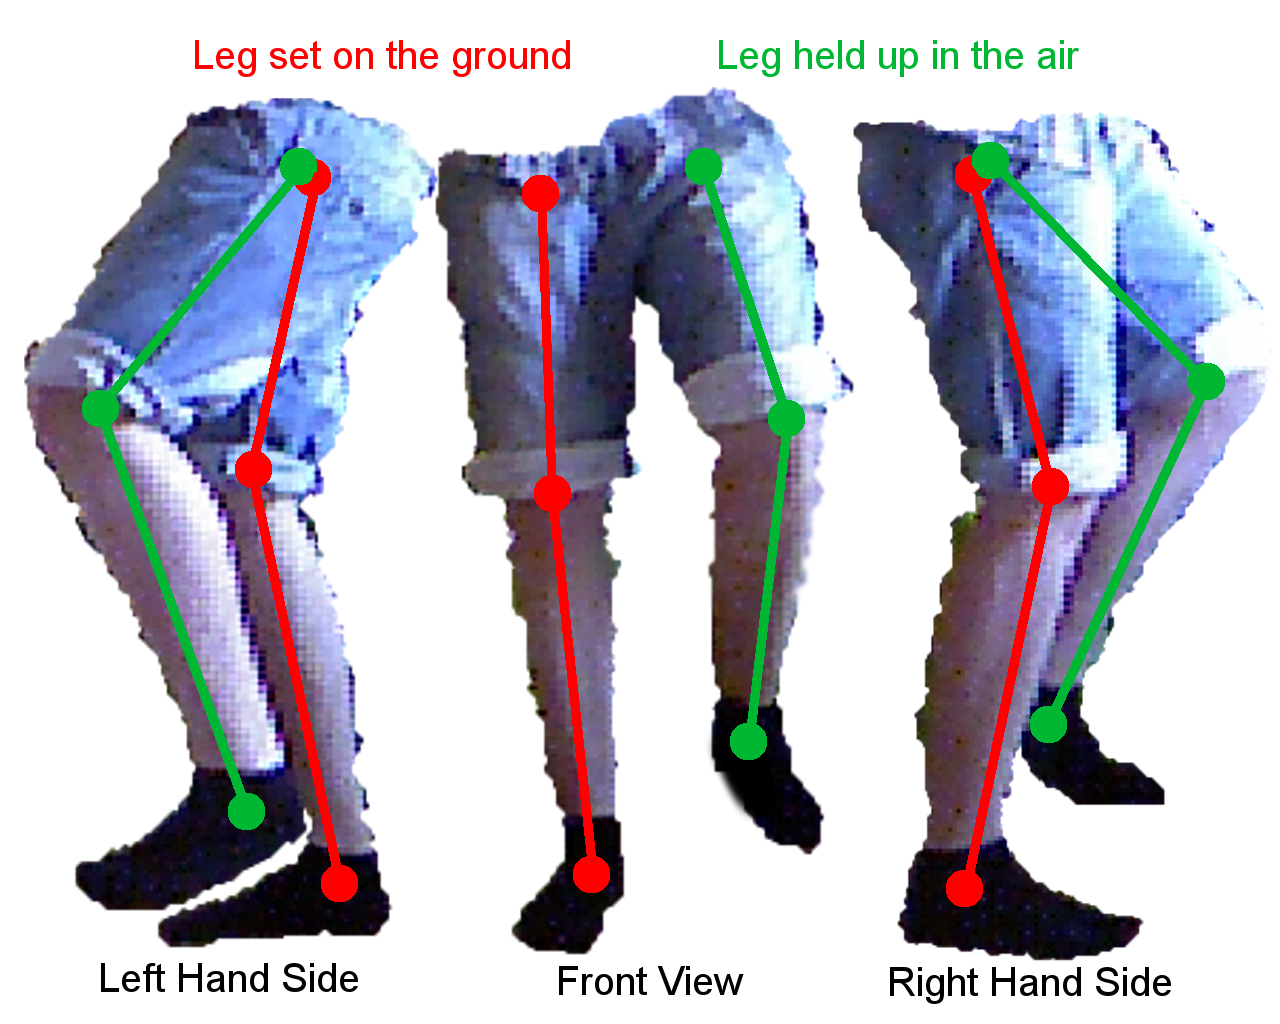
\includegraphics[height=0.4\linewidth]{figures/3-IMR/rehabilitationstance}}
	\subfloat[The lifted leg is not in the limited area.]{\label{fig:3-IMR:rehabilitationstance:b} 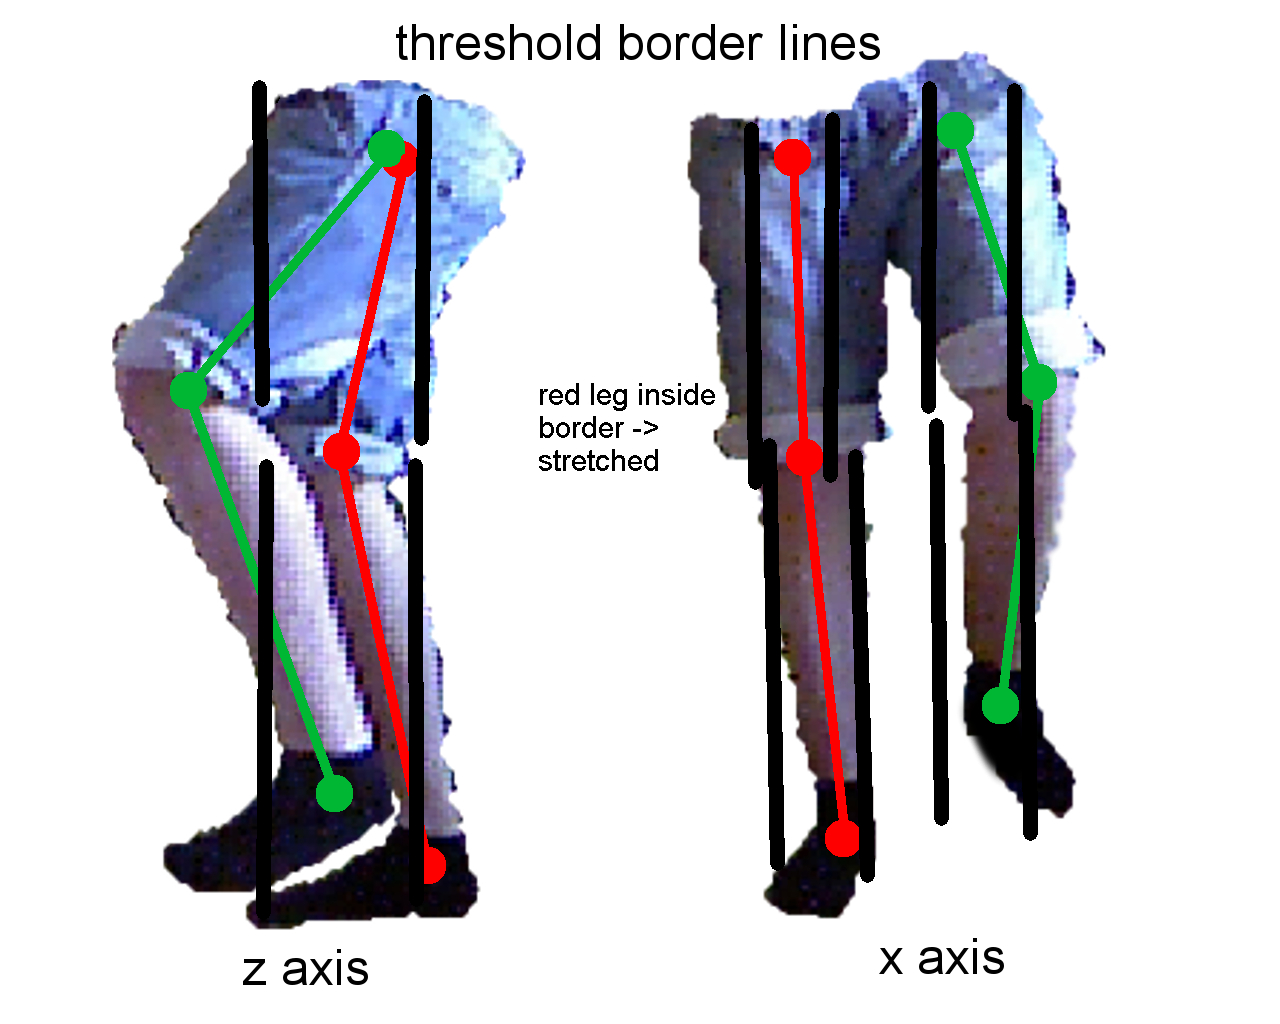
\includegraphics[height=0.4\linewidth]{figures/3-IMR/rehabilitationstance2}}
	\caption{Stance detection. The system has to detect which leg the patient is standing on and the particular standing pose.}
	\label{fig:3-IMR:rehabilitationstance}
\end{figure}
The first approach cannot detect the lifted leg if the foot is held very still in the air. To supplement this case, a second approach is proposed. The program calculates a limited area for each leg according to the ground plane and the hip positions. If it detects that any leg joint is exceeding the limited area more than a threshold, it is considered lifted as well (see \figurename{\ref{fig:3-IMR:rehabilitationstance:b}}). The limited area and threshold are adjusted to the size of the person. 
The limited area is marked by black lines. 
A stable solution is to combine both approaches to detect the lifted leg.
To ensure that the knee is bent properly, the angle between the three dimensional ``Knee-Ankle'' and the ``Knee-Hip'' vectors is calculated (see \figurename{\ref{fig:3-IMR:rehabilitationKneeAngle}}). If this angle gets over $175\degree$, the leg can no longer be considered bent. Bending the leg too much also can be detected with this method.
\begin{figure}
	\centering
	\subfloat[Angle of the bent Knee.]{
		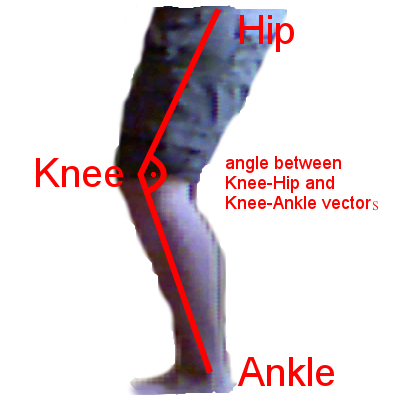
\includegraphics[height=0.4\linewidth]{figures/3-IMR/rehabilitationKneeAngle}\label{fig:3-IMR:rehabilitationKneeAngle}
		}
	\quad
	\subfloat[Player not standing with straight upper body.]{
		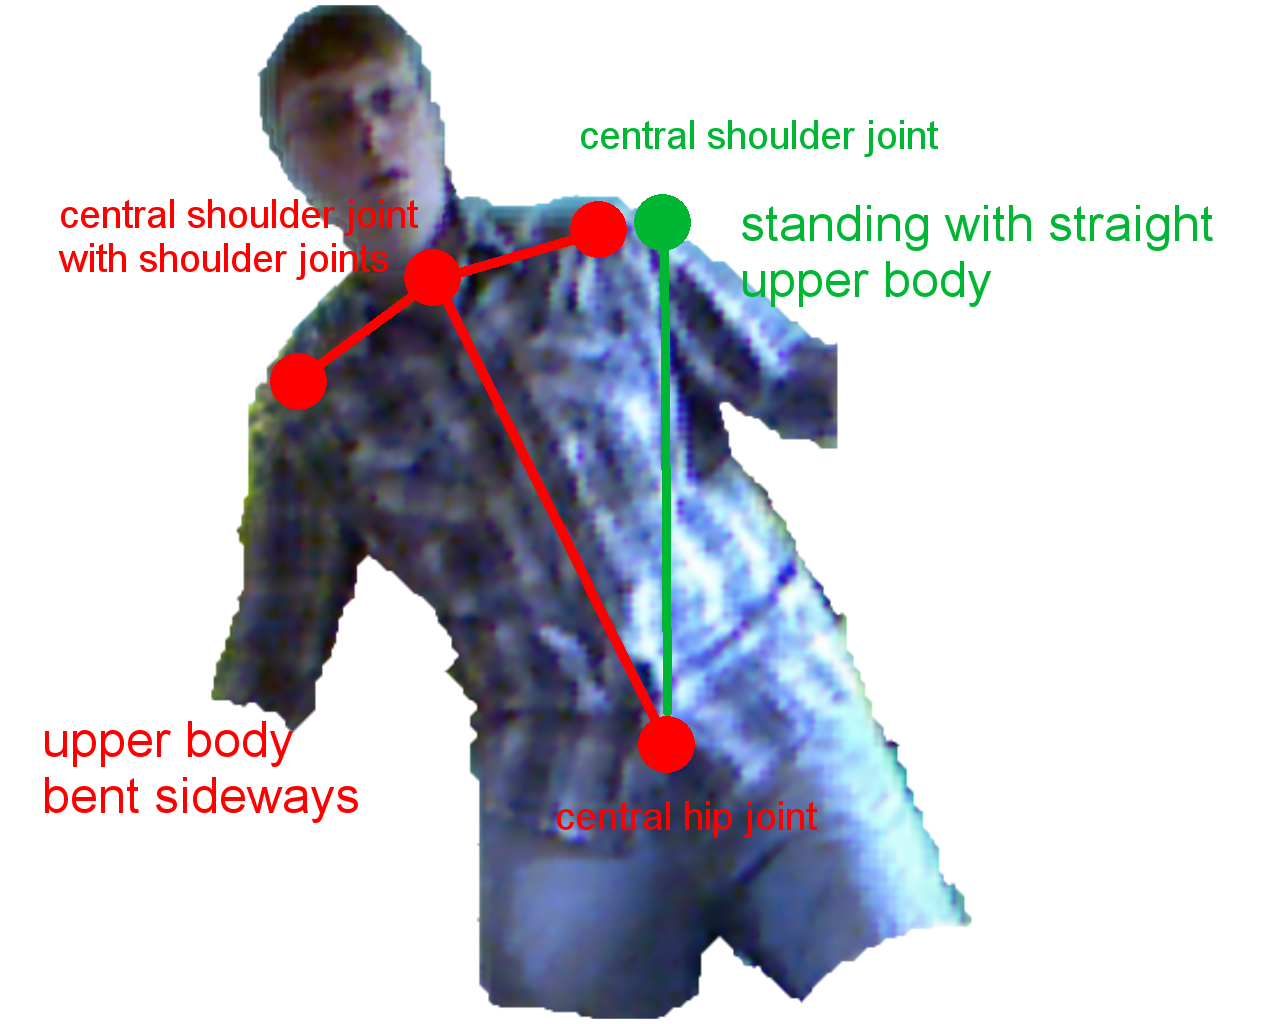
\includegraphics[height=0.4\linewidth]{figures/3-IMR/rehabilitationSraight}
		\label{fig:3-IMR:rehabilitationSraight}
		}
	\caption{Detection of stance states. Angle of the bent Knee is calculated based on the skeletal joint position and the spine direction is calculated to check if the user stands straightly.}
	\label{fig:3-IMR:poseDetection}
\end{figure}

\paragraph{Detection of unstable stances}
The objective of the balance rehabilitation is that the patient can keep the upper body stable while standing with one leg or on a balance board. The system has to detect if the upper body is kept straight all the time.  A large change of the shoulder position can be also used to check if the user has lost their balance. The spine direction also has to be calculated to check if it still remains as straight.
It calculates the vector from the shoulder center (neck) to the center of the hips. For a person standing straight, the vector should be perpendicular to the ground plane. The angle  between the vector and plane is calculated to estimate the state of the upper body (see \figurename{\ref{fig:3-IMR:rehabilitationSraight}}). 
Normal movement should not instantly be detected as loss of balance, such as small movements to keep balance. Large, fast movements or twisting of the body however need to be detected. The person in \figurename{\ref{fig:3-IMR:rehabilitationSraight}} is not standing straight and has lost his balance. The user then has to be notified and prompted to correct his stance and regain balance.
The length of the vector between the center of the shoulders and the center between the hips is calculated and used to calculate appropriate thresholds. 
The game should be able to be played by patients in different states of their rehabilitation. For this, it has to offer a certain threshold of customization. The customization mainly includes restrictions to stances allowing an easier start for the patient. For patients who are further advanced in the rehabilitation process, it can offer a challenge setting.
%This is done by dividing the length of the vector with a heuristically determined variable. 

\paragraph{Stance correction}
This function provides feedback to the patient after detection of incorrect pose and unstable stance. The feedback can be printed on the screen as a normal message and special sound to attract the attention of the user.
Instead of an error message, which discourages the user, the system tells the patient what to do to recover the correct pose.
When a balance violation is first detected, one hint message is generated to recover the balance. Then the message is shown on the screen and a special sound effect is played to attract the attention of the user. These messages are displayed for a configurable amount of time. While one message is displayed, no other message can overwrite it. We think displaying multiple correction messages would confuse the patient. 
The new message is allowed to overwrite the existing message before the predefined time or when the correct pose is recovered.
The system also has to detect the case when both legs remain on the ground and then the patient has to receive a message that asks them to lift one of their legs. 
If this rule for bent legs is violated, another message is displayed to tell the patient how to recover it.

\paragraph{MR scenarios}
An MR scenario is designed to motivate the patient following the general rules for games. 
Based on information from the Kinect sensor, a segmentation of the patient's body in color image is generated. A virtual background image is displayed in the Magic Mirror to generate a MR environment (see \figurename{\ref{fig:3-IMR:rehabilitationGame}}).  
%Combining the color image with the background image is done by alpha blending. Every pixel of the texture is tested with the alpha mask provided by the user segmentation. This alpha mask has a high value for pixels belonging to the segmentation. Every single pixel is tested with these values and the resulting blend value is stored in a new bitmap. This bitmap then is rendered to the screen and generate a virtual background.
To motivate the patient to continue playing the game, a wide variety of themes are offered. The background image, target object and its movement patterns are thematically designed to create a new experience for a different theme. Sound effect is also employed to enhance the experience of the players. 
The scenarios can either be unlocked after achieving a certain proficiency at the game, e.g. achieving a certain amount of score, or be available from the beginning to offer a wide variety of choices to the user. 

\begin{figure}
	\centering
	\includegraphics[width = \linewidth]{figures/3-IMR/rehabilitationGame}
	\caption{Rehabilitation gaming. \add{ A virtual background image is displayed in the Magic Mirror to generate a MR environment and a user tries to catch the moving objects around him.}}
	\label{fig:3-IMR:rehabilitationGame}
\end{figure}
\paragraph{Difficulty level}
Games usually offer variety, challenges, and difficulty levels, and rewards the player if he or she overcomes the difficulties and challenges.
Our game offers difficulty settings that are configurable independently for every limb. The difficulty influences the speed as well as the patterns of the moving targets. Higher difficulty means higher speed and more complex movement patterns.
The player starts with an easy basic mode and continues with more difficult levels after achieving a special objective or a certain amount of score. 
%The Beach scenario is easy with only one easy movementpattern for the objects, while the Football scenario has balls flying with relatively high speeds from different directions towards the player. The spaceship scenario is intended as the final mode with objects that do not disappear after they reach a certain point. It offers the highest score and an unique experience without time pressure which makes it easier to follow the complicated movement patterns.

\paragraph{Rewarding score} During the game, the player gets rewarded when the balance is kept continuously for a period of time. The system also decreases the score when a incorrect pose is detected. 
The score for each target is set according to the difficulty and the scenario. The easier the mode, the less score gets awarded. The final score gives the player a sense of accomplishment while also gaining a way to compare their performance in the game with previous gaming performances. 

\subsubsection{Conclusion}
The mixed reality game is more immersed and interactive than normal exercises and thus offers enjoyment while doing rehabilitation exercises, motivating the patient. Playing an MR game helps the user to generate a sense of enjoyment when doing rehabilitation exercises. Having fun through exercises can motivate the patient to perform their exercises more frequently. The Magic Mirror concept also offers the users to observe themselves as looking into a mirror to perceive the wrong stances. The visual and sound feedback provides them instant hints to recover the correct pose. With the help of this system, the patient would be able to do exercises at home without being constantly monitored by a physiotherapist. All the data about the exercise can be collected and analyzed by the physiotherapist later via WiFi transmission for example.